%%%%%%%%%%%%%%%%%%%%%%%%%%%%%%%%%%%%%%%%%
% Beamer Presentation
% LaTeX Template
% Version 1.0 (10/11/12)
%
% This template has been downloaded from:
% http://www.LaTeXTemplates.com
%
% License:
% CC BY-NC-SA 3.0 (http://creativecommons.org/licenses/by-nc-sa/3.0/)
%
%%%%%%%%%%%%%%%%%%%%%%%%%%%%%%%%%%%%%%%%%

%----------------------------------------------------------------------------------------
%	PACKAGES AND THEMES
%----------------------------------------------------------------------------------------

\documentclass{beamer}

\mode<presentation> {

% The Beamer class comes with a number of default slide themes
% which change the colors and layouts of slides. Below this is a list
% of all the themes, uncomment each in turn to see what they look like.

%\usetheme{default}
%\usetheme{AnnArbor}
%\usetheme{Antibes}
%\usetheme{Bergen}
%\usetheme{Berkeley}
%\usetheme{Berlin}
%\usetheme{Boadilla}
%\usetheme{CambridgeUS}
%\usetheme{Copenhagen}
%\usetheme{Darmstadt}
%\usetheme{Dresden}
%\usetheme{Frankfurt}
%\usetheme{Goettingen}
%\usetheme{Hannover}
%\usetheme{Ilmenau}
%\usetheme{JuanLesPins}
%\usetheme{Luebeck}
\usetheme{Madrid}
%\usetheme{Malmoe}
%\usetheme{Marburg}
%\usetheme{Montpellier}
%\usetheme{PaloAlto}
%\usetheme{Pittsburgh}
%\usetheme{Rochester}
%\usetheme{Singapore}
%\usetheme{Szeged}
%\usetheme{Warsaw}

% As well as themes, the Beamer class has a number of color themes
% for any slide theme. Uncomment each of these in turn to see how it
% changes the colors of your current slide theme.

%\usecolortheme{albatross}
%\usecolortheme{beaver}
%\usecolortheme{beetle}
%\usecolortheme{crane}
%\usecolortheme{dolphin}
%\usecolortheme{dove}
%\usecolortheme{fly}
%\usecolortheme{lily}
%\usecolortheme{orchid}
%\usecolortheme{rose}
%\usecolortheme{seagull}
%\usecolortheme{seahorse}
%\usecolortheme{whale}
%\usecolortheme{wolverine}

%\setbeamertemplate{footline} % To remove the footer line in all slides uncomment this line
%\setbeamertemplate{footline}[page number] % To replace the footer line in all slides with a simple slide count uncomment this line

%\setbeamertemplate{navigation symbols}{} % To remove the navigation symbols from the bottom of all slides uncomment this line
}
\usepackage[utf8]{inputenc}
\usepackage[english]{babel}
\usepackage{graphicx} % Allows including images
\usepackage{booktabs} % Allows the use of \toprule, \midrule and \bottomrule in tables
\usepackage[]{circuitikz}
\usepackage{amsbsy,bm,amsmath} % math formatting
\usepackage{graphicx,subfig,float,wrapfig,rotating,multirow,epstopdf} %high quality tables and images 

\graphicspath{{img/}} % Set graphics directory


%----------------------------------------------------------------------------------------
%	TITLE PAGE
%----------------------------------------------------------------------------------------

\title[Gilbert Cell Design]{Analog Integrated Circuits \\
	\huge {\textsc{Analysis and design of a double balanced Gilbert Cell Based Mixer in AMI06 technology}}} % The short title appears at the bottom of every slide, the full title is only on the title page

\author{Enrico Maria Renzi\\Roberto Rubino } % Your name
\institute[PoliTo] % Your institution as it will appear on the bottom of every slide, may be shorthand to save space
{
Politecnico di Torino \\ % Your institution for the title page
\medskip
% \textit{john@smith.com} % Your email address
}
\date{\today} % Date, can be changed to a custom date

\begin{document}

\begin{frame}
\titlepage % Print the title page as the first slide
\end{frame}

\begin{frame}
\frametitle{Overview} % Table of contents slide, comment this block out to remove it
\tableofcontents % Throughout your presentation, if you choose to use \section{} and \subsection{} commands, these will automatically be printed on this slide as an overview of your presentation
\end{frame}


%----------------------------------------------------------------------------------------
%	PRESENTATION SLIDES
%----------------------------------------------------------------------------------------
\section{Analog multipliers theory}

\subsection{Introduction}
\begin{frame} % display current subsection in subindex
\tableofcontents[currentsubsection]
\end{frame}


% new slide
\begin{frame}
	\frametitle{Analog multipliers working principles}
	\textbf{Analog Multiplier} circuit that performs the product between two signals. Spectral components from a certain frequency band are moved to another by means of intrinsic non-linear behaviour (modulation). The working principle is below:
	\begin{figure}[H]
	\centering
	\scalebox{0.78}
	{
		\begin{circuitikz} 
			\ctikzset{tripoles/mos style/arrows,bipoles/length=1cm}
			\draw
			(0,0) node[mixer] (m) {}
			(m.1) to[short,-] ++(-.5,0) node[left]{$x_1(t)= A_1 \cos(\omega_1 t + \varphi_1)$}
			(m.2) to[short,-] ++(0,-.5) node[below]{$x_2(t) = A_2 \cos(\omega_2 t + \varphi_2)$}
			(m.3) to[short,-] ++(.5,0) node[inputarrow]{} (.5,0) node[right=3mm]{$y(t)= \frac{A_1 A_2}{2} \cos(\omega_{LF} t + \varphi_{LF}) +\frac{A_1 A_2}{2} \cos(\omega_{HF} t + \varphi_{HF})$}
			(m.1) node[inputarrow] {} 
			(m.2) node[inputarrow,rotate=90] {};
		\end{circuitikz}
	}		
	\label{Mixer2}	
	\end{figure}
	Two \textbf{new} out-of-phase spectral component at output:
	\begin{description}
		\item[Down-converted] at lower frequency: $\omega_{LF}= |\omega_1-\omega_2|<\omega_1,\omega_2 $
		\item[Up-converted] at higher frequency: $\omega_{HF}= |\omega_1+\omega_2|>\omega_1,\omega_2$
	\end{description}


	
\end{frame}


% new slide
\begin{frame}
	\frametitle{Analog multipliers working principles}
	Mixers are \emph{bi-direction} three-port. At each port a signal is associated
	\begin{description}
		\item[RF]  radio frequency component, high frequency signal;
		\item[IF] intermediate frequency component, low frequency signal;
		\item[LO]  local oscillator (pump), provided by external source.
	\end{description}
	Depending on input/output signal configuration we can have \emph{downconverting} or \emph{upconverting} modulators.
	
		\begin{figure}[H]
			\centering
			\scalebox{0.9}
			{
				\begin{circuitikz} 
					\ctikzset{tripoles/mos style/arrows,bipoles/length=1cm}
					\draw
					(0,0) node[mixer] (m) {}
					(m.1) to[short,-] ++(-.5,0) node[left]{RF}
					(m.2) to[short,-] ++(0,-.5) node[below]{LO}
					(m.3) to[short,-] ++(.5,0) node[inputarrow]{} (.5,0) node[right=3mm]{IF}
					(m.1) node[inputarrow] {} 
					(m.2) node[inputarrow,rotate=90] {};
					\draw
					(6,0) node[mixer] (m) {}
					(m.1) to[short,-] ++(-.5,0) node[left]{IF}
					(m.2) to[short,-] ++(0,-.5) node[below]{LO}
					(m.3) to[short,-] ++(.5,0) node[inputarrow]{} (6.5,0) node[right=3mm]{RF}
					(m.1) node[inputarrow] {} 
					(m.2) node[inputarrow,rotate=90] {};
				\end{circuitikz}
			}	
			\caption{Working configuration: downconversion (right), upconversion (left).}	
			\label{Mixerdown}	
		\end{figure}

		
	
\end{frame}

% new slide
\begin{frame}
	\frametitle{Mixer figures of merit}
	To qualify the mixer operation some figures of merit are defined (downconversion mixer):
	\begin{itemize}
		\item \textbf{Conversion gain}
		\begin{equation}
			A_{conv}=\frac{P_{IF}}{P_{RF}} \notag 
		\end{equation}
		whose behaviour is linear in log scale:
		\begin{equation}
			P_{IF}|_{dB_{m}} = A_{conv}|_{dB} + P_{RF}|_{dB_{m}}+30dB \notag
		\end{equation}
		\item \textbf{1dB compression point} defines the input power level for which the difference between the compressed and non-compressed output power is 1dB. It is due to gain saturation caused by harmonic distortion:
		\begin{equation}
			P_{IF}|_{-1dB} = P_{IF}|_{dB_{m},ideal} -1dB \notag
		\end{equation} 
	\end{itemize}
\end{frame}

% new slide
\begin{frame}
	\frametitle{Mixer figures of merit}
	\begin{itemize}
		\item \textbf{Third order distortion} most important output spurious contribution due to gain compression:
		\begin{align}
			i_D(t) &= I_D|_{V_{GS}}+av_{gs}(t)+bv_{gs}^2(t)+cv_{gs}^3(t)+\dots \notag \\
			& \propto av_{gs}(t)+bv_{gs}^2(t)+\frac{3}{4}c\cos(\omega_0 t) +\frac{1}{4}c\cos(3\omega_0 t) \notag
		\end{align}
		Even order distortion gives additional DC offset, odd order distortion gives always in-band unwanted components.
		\item \textbf{Third order intermodulation} it happens with two-tone input signals because of frequency intermodulation. Most important contribution comes from IM\textsubscript{3}: $m=\pm2,\pm1$ and $n=\pm2,\pm1$. Given $f_{RF1} = f_0$ and $f_{RF2}=f_0+\delta f$:
		\begin{equation}
			f_{IF,IM3}|_{\substack{m=2\\n=-1}} = 2f_{RF1} - f_{RF2} -f_{LO}= f_{IF} - \delta f \notag
		\end{equation} 
	\end{itemize}
\end{frame}

\subsection{Analysis of a Gilbert cell based multiplier}

% new slide
\begin{frame} % display current subsection in subindex
\tableofcontents[currentsubsection]
\end{frame}

\begin{frame}
	\frametitle{Gilbert cell overview}
	A Gilbert-cell mixer is an active double-balanced analog multiplier. This topology provides:
	\begin{itemize}
		\item Reasonable conversion gain;
		\item Good rejection of input frequency components at the output port, high linearity;
		\item Good isolation between ports;
		\item Integrability in CMOS technology.
	\end{itemize}
	We can recognise \textbf{four main blocks}: bias net, gain stage, mixing stage and load. 
\end{frame}

%new slide
\begin{frame}
\frametitle{Gilbert cell circuit analysis - Bias net}
\begin{figure}[H] 
	\centering
	\subfloat[][\emph{Bias net}]{\scalebox{0.6}{\begin{circuitikz}
				\ctikzset{tripoles/mos style/arrows,bipoles/length=1cm}
				\ctikzset{bipoles/capacitor/height=0.5}
				\ctikzset{bipoles/capacitor/width=0.1}
				%M2
				\draw (0,0) to[Tnmos,mirror,n=M2] (0,2);
				\draw (M2.source) node[left=3mm,above=3mm]{$M2$};
				\draw (M2.gate)[right] |- (M2.drain);
				\draw (M2.gate) to[short,-*] (2.5,1) node[right]{to $G_1$};
				\draw (M2.source) to[short] (0,0) node[sground]{};
				\draw (0,6) -- (-2,6) to[C=$C_{bias}$] (-2,5) node[sground]{};
				%M5
				\draw (M2.drain) to[Tnmos,mirror,n=M5] (0,4.5);
				\draw (M5.source) node[left=3mm,above=3mm]{$M5$};
				\draw (M5.gate)[right] |- (M5.drain);
				\draw (0,4) -- (-2,4) to[C=$C_{bias}$] (-2,3) node[sground]{};
				\draw (M5.gate) to[R, l_=$R_1$] (2,2.3) to[short,-*] (2.5,2.3) node[right]{to $G_3$};
				\draw (M5.gate) to[R=$R_1$] (2,3.7) to[short,-*] (2.5,3.7) node[right]{to $G_4$};
				%R2 R4
				\draw (M5.drain) to[R=$R_2$,n=R2] (0,6.3) to[R=$R_4$] (0,7.1) to[short,-*] (0,7.5) node[above]{$V_{dd}$};
				\draw (0,5.7) to[short] (0.7,5.7) to[R,l_=$R_3$] (2,5) to[short,-*] (2.5,5) node[right]{to $G_6$,$G_9$};
				\draw (0,5.7) to[short] (0.7,5.7) to[R=$R_3$] (2,6.4) to[short,-*] (2.5,6.4) node[right]{to $G_7$,$G_8$};
	\end{circuitikz}}} \quad
	\subfloat[][\emph{Gilbert cell}]{\scalebox{0.6}{\begin{circuitikz}
				\ctikzset{tripoles/mos style/arrows,bipoles/length=1cm}
				\ctikzset{bipoles/capacitor/height=0.5}
				\ctikzset{bipoles/capacitor/width=0.1}
				%drawing MOS
				\draw (0,0) to[Tnmos,n=M1] (0,2)
				(M1.source) node[right=3mm, above=3mm]{$M1$};
				\draw (M1.gate) to[short,-*] (-1,1);
				
				\draw (0,2) to[R,l=$R_S$] (-2,2)
				to[Tnmos,n=M3] (-2,4)
				(M3.source) node[right=3mm, above=3mm]{$M3$};
				
				\draw (0,2) to[R,l_=$R_S$] (2,2) to[Tnmos,mirror,n=M4] (2,4)
				(M4.source) node[left=3mm, above=3mm]{$M4$};
				
				\draw (-2,4) -- (-3,4)
				to[Tnmos,n=M6] (-3,5.5)
				(M6.source) node[right=3mm, above=3mm]{$M6$};
				
				\draw (-2,4) -- (-1,4) to[Tnmos,mirror,n=M7] (-1,5.5)
				(M7.source) node[left=3mm, above=3mm]{$M7$};
				
				\draw (2,4) -- (1,4) to[Tnmos,n=M8] (1,5.5)
				(M8.source) node[right=3mm, above=3mm]{$M8$};
				
				\draw (2,4) -- (3,4) to[Tnmos,mirror,n=M9] (3,5.5)
				(M9.source) node[left=3mm, above=3mm]{$M9$};
				
				%drawing VLO-
				\draw (M7.gate) -- (M8.gate);
				\draw (M7.gate) -| (0,4.5);
				\draw (0,4.5) to[C=$C_{signal}$] (0,3) to[short,-*] (0,3) node[below]{$V_{LO}-$};
				
				%drawing RL and out connections
				\draw (M6.drain) -- (-3,6) to[R=$R_L$,n=RL1] (-3,7) -- (-3,7.5);
				\draw (M9.drain) --(3,6) to[R=$R_L$,n=RL2] (3,7) -- (3,7.5);
				\draw (-1,5.5) -- (3,6);
				\draw (1,5.5) -- (-3,6);
				
				%Vdd and ground
				\draw (-3,7.5) node[above=3mm,right=3cm]{$V_{dd}$} -- (3,7.5);
				\draw (M1.source) -- (0,0) node[sground]{};
				
				% VLO+-
				\draw (M6.gate) -| (-4,4.75) to[short,-*] (-4,4.75) node[left]{to $G9$};
				%-| (-4,4.7) to[short,-*] (-4,3) node[left]{to $G_9$};
				\draw (M9.gate) -| (4,4.7) to[C=$C_{signal}$] (4,3) to[short,-*] (4,3) node[below]{$V_{LO}+$};
				
				% VRF+-
				\draw (M3.gate) -| (-3,2) to[C, l_=$C_{signal}$] (-3,1) to[short,-*] (-3,0.5) node[left]{$V_{RF}+$};
				\draw (M4.gate) -| (3,2) to[C, l_=$C_{signal}$] (3,1) to[short,-*] (3,0.5) node[left]{$V_{RF}-$};
				%\draw (M4.gate) -- (3,3) to[short,-*] (3,3) node[right]{$V_{RF}-$};
				
				%Out nodes
				\draw (-3, 6) to[short,*-*] (-4, 6) node[left]{$V_{out}+$};
				\draw (3, 6) to[short,*-*] (4, 6)node[right]{$V_{out}-$};
	\end{circuitikz}}}
	\caption{Full schematic}
	\label{fig:TdomaniDFT}
\end{figure}
\end{frame}

\begin{frame}
	\frametitle{Gilbert cell circuit analysis - Bias net}
	Ideally current mirroring only dependent on \textbf{geometrical} parameters. However, in real circuits:
	\begin{itemize}
		\item To have good current source long channel required, since $r_o=1/\lambda I_0\propto L$. Using short channel devices i\textsubscript{D} more dependent on $\lambda$ and tolerances;
		\item Due to fabrication precision, MOSFET's parameters may vary:
		\begin{equation}
		\frac{I_0}{I_{REF}} \simeq 1 + \frac{\Delta K_n}{K_n}+2\frac{\Delta V_{th}}{V_{od}} \notag
		\end{equation}
	\end{itemize}
	Wide circuits, temperature gradients and small overdrive voltage significantly induce mirroring errors.
\end{frame}

\begin{frame}
	\frametitle{Gilbert cell circuit analysis - Gain stage}
	\begin{columns} [c]
		\column{.45\textwidth}
		Thanks to source degeneration we reduce bias dependency and  increase \textbf{linearity} (high order harmonics suppression).
		\begin{equation}
		\label{eq_degenGain}
		G_{m,eq} = \frac{g_m}{1+g_m R_S} \notag
		\end{equation}
		\column{.5\textwidth}
		\begin{figure}[H]
			\centering
			\scalebox{0.8}{
			\begin{circuitikz}
				\ctikzset{tripoles/mos style/arrows,bipoles/length=1cm}
				%I_0 and RS
				\draw (0,0) to[short,i<=$I_0$] (0,1);
				\draw (0,1) to[R,l_=$R_S$] (-1,1) -| (-1.5,1.5) to[Tnmos,n=M3] (-1.5,2) to[twoport,l=$LO_{stage}$] (-1.5,4);
				\draw (M3.source) node[right=3mm, above=3mm]{$M3$};
				\draw (0,1) to[R,l=$R_S$] (1,1) -| (1.5,1.5) to[Tnmos,n=M4,mirror] (1.5,2) to[twoport,l=$LO_{stage}$] (1.5,4);
				\draw (M4.source) node[left=3mm, above=3mm]{$M4$};
				\draw (M3.gate) -| (-2.5,1.7) to[short,-*] (-2.5,1.75) node[below]{$V_{in1}$};
				\draw (M4.gate) -| (2.5,1.7) to[short,-*] (2.5,1.75) node[below]{$V_{in2}$};
				%Vx Vy
				\draw (M3.drain) -| (-1,2.3) to[short,-*] (-1,2.3) node[right]{$V_x$};
				\draw (M4.drain) -| (1,2.3) to[short,-*] (1,2.3) node[left]{$V_x$};
			\end{circuitikz}
			}
			\caption{Gain stage.}
			\label{fig:GainStage}
		\end{figure}
	\end{columns}
\end{frame}


\begin{frame}
	\frametitle{Gilbert cell circuit analysis - Mixing stage}
	\begin{figure} [H]
		\centering
		\scalebox{0.6}{
		\begin{circuitikz}
			\ctikzset{tripoles/mos style/arrows}
			\draw (-2,4) -- (-3,4)
			to[Tnmos,n=M6] (-3,5.5)
			(M6.source) node[right=3mm, above=5mm]{$M6$};
			
			\draw (-2,4) -- (-1,4) to[Tnmos,mirror,n=M7] (-1,5.5)
			(M7.source) node[left=3mm, above=5mm]{$M7$};
			
			\draw (2,4) -- (1,4) to[Tnmos,n=M8] (1,5.5)
			(M8.source) node[right=3mm, above=5mm]{$M8$};
			
			\draw (2,4) -- (3,4) to[Tnmos,mirror,n=M9] (3,5.5)
			(M9.source) node[left=3mm, above=5mm]{$M9$};
			
			%drawing VLO-
			\draw (M7.gate) -- (M8.gate);
			\draw (M7.gate) -| (0,4.5);
			\draw (0,4.5) to[short,-*] (0,3) node[below]{$V_{LO}-$};
			
			%Out nodes
			\draw (-3, 6) to[short,*-*] (-4, 6) node[left]{$V_{out}+$};
			\draw (3, 6) to[short,*-*] (4, 6)node[right]{$V_{out}-$};
			\draw (M6.drain) to[short] (-3,7);
			\draw (M6.gate) -| (-4,3) to[short,-*] (-4,3) node[below]{$V_{LO}+$};
			\draw (M7.drain) -- (3,6);
			\draw (M8.drain) -- (-3,6);
			\draw (M9.drain) to[short] (3,7);
			\draw (M9.gate) -| (4,3) to[short,-*] (4,3) node[below]{$V_{LO}+$};
			\draw (-2,3) -- (-2,4)
			(2,3) -- (2,4);
		\end{circuitikz}
		}
		\caption{Mixing stage}
		\label{fig:MixStage}
	\end{figure}
	Mixing stage is made up of switching-like driven transistors that acts as \textbf{pulse amplitude modulators}. % PAM is different from PWM!!!!!!!!
	A complementary sinusoidal signal is applied to the gates of each pair (V\textsubscript{LO}), large enough to ensure the \textbf{abrupt switching} of one MOSFET whereas the other must be kept in saturation (not in  triode!).
\end{frame}

\begin{frame}
	\frametitle{Gilbert cell circuit analysis - Mixing stage}
	Compromise in driving signal required:
	\begin{itemize}
		\item small LO signals produce slower switching speed and reduces efficiency (as common mode signal at the output);
		\item large LO signals drive the device in triode (spikes and unwanted feed-through reducing gain).
	\end{itemize}
	Switching speed is related to MOSFET transition frequency:
	\begin{equation}
	f_T \propto  V_{od}/L \notag
	\end{equation}
	Then fast devices are obtained with \textbf{short channel} length and \textbf{large overdrive}. Larger devices introduce parasitic capacitance, detrimental for the conversion efficiency and speed. Maximum working frequency should be below $f_T/10$.
\end{frame}

\begin{frame}
	\frametitle{Gilbert cell circuit analysis - Mixing stage}
	Mixing stage is non linear, however given the square wave current flowing through each device:
	\begin{equation}
	i_D(t)=I_{pk}\Bigg(\frac{1}{2}-\frac{2}{\pi} \sum_{n=1,3,5 \dots}^{} \frac{1}{n}\sin(n\omega t)\Bigg) \notag
	\end{equation} 
	one has the instantaneous gain:
	\begin{equation}
	\label{eq_SwitchGain}
	A_c|_{switch} = \frac{2}{\pi} \notag
	\end{equation}
	associated to first harmonic, ideally not depending on device properties. For real devices the actual gain is lower.
\end{frame}

\begin{frame}
	\frametitle{Gilbert cell circuit analysis - Load stage}
	Two resistors are employed as loads. They are less noisy than transistors (Flicker noise at low frequency), less reliable for what concern tolerances though. They are required to provide enough gain to the stage, if necessary active loads can be employed to maximize gain.
\end{frame}

\begin{frame}
	\frametitle{Gilbert cell circuit analysis - Conversion gain}
	The circuit is non-linear, therefore it is not possible to define a gain. It can be demonstrated that the static \textbf{conversion gain} for the cell is:
	\begin{equation}
	\label{eq:ConvGain}
	A_{vC} = \frac{V_{IF,rms}}{V_{RF,rms}} =  \frac{2}{\pi}\frac{R_L}{\frac{1}{g_{m3,4}}+R_S} \simeq \frac{2}{\pi}\frac{R_L}{R_S} \notag
	\end{equation}
	Some important facts hold:
	\begin{itemize}
		\item in first approximation the conversion gain does not depend on the amplitude of the LO signal;
		\item both LO and RF components are rejected at the output;
	\end{itemize}  
\end{frame}
\section{Circuit design}

\subsection{Design by hand of a down-converting Gilbert cell}
\begin{frame} % display current subsection in subindex
\tableofcontents[currentsubsection]
\end{frame}

\begin{frame}
\frametitle{Design specifications}
\begin{block}{Technology and purposes}
Technology used is MOSIS AMI 0.6$\mu$m. Loose constraint of $\sim 1mm$ is taken for maximum gate width. This technology is old fashioned and not the best for this purpose.
\end{block}

\begin{block}{Supply voltage}
Supply voltage is chosen $5V$ 
\end{block}

\begin{block}{Frequencies}
Single frequency down-converting mixer with: \\ f\textsubscript{RF}=110 MHz, f\textsubscript{LO}=100 MHz, f\textsubscript{IF}=10 MHz.
\end{block}
\begin{block}{Conversion Gain}
Voltage conversion gain is chosen A\textsubscript{vC}=4. All transistors are supposed in saturation.
\end{block}
\end{frame}

\begin{frame}
\frametitle{Used parameters}
\begin{table} [h]
\label{tab:specs}
\caption{}
\centering	
\begin{tabular}{llcc} 
\toprule 
Parameter & Name			& Value 	& Unit \\ 
\midrule
A\textsubscript{vC} & Voltage Conversion gain & 4 & \\
V\textsubscript{DD} & Supply voltage &	5 & V		\\
I\textsubscript{0} & Cell biasing current & 5 & mA \\
V\textsubscript{th0} & n-MOS threshold w.o. body effect& 0.709 &V		\\ 
K\textsubscript{n} & n-MOS physical parameter& 116 & $\mu$A/V\textsuperscript{2}\\
I\textsubscript{dss} & Maximum channel current density & 466 & $\mu$A/$\mu$m \\
$\phi_P$ & Fermi potential & 0.7 & V \\
$\gamma_B$ & Body effect coefficient & 0.5 & V \\
L\textsubscript{min} & Technology minimum length & 0.6 & $\mu$m \\
\bottomrule 
\end{tabular}	
\end{table}	
\end{frame}

\begin{frame}
\frametitle{Reference schematic}
\begin{figure}[H] 
\centering
\subfloat[][\emph{Bias net}]{\scalebox{0.7}{\begin{circuitikz}
			\ctikzset{tripoles/mos style/arrows,bipoles/length=1cm}
			\ctikzset{bipoles/capacitor/height=0.5}
			\ctikzset{bipoles/capacitor/width=0.1}
			%M2
			\draw (0,0) to[Tnmos,mirror,n=M2] (0,2);
			\draw (M2.source) node[left=3mm,above=3mm]{$M2$};
			\draw (M2.gate)[right] |- (M2.drain);
			\draw (M2.gate) to[short,-*] (2.5,1) node[right]{to $G_1$};
			\draw (M2.source) to[short] (0,0) node[sground]{};
			\draw (0,6) -- (-2,6) to[C=$C_{1}$] (-2,5) node[sground]{};
			%M5
			\draw (M2.drain) to[Tnmos,mirror,n=M5] (0,4.5);
			\draw (M5.source) node[left=3mm,above=3mm]{$M5$};
			\draw (M5.gate)[right] |- (M5.drain);
			\draw (0,4) -- (-2,4) to[C=$C_{2}$] (-2,3) node[sground]{};
			\draw (M5.gate) to[R, l_=$R_1$] (2,2.3) to[short,-*] (2.5,2.3) node[right]{to $G_3$};
			\draw (M5.gate) to[R=$R_1$] (2,3.7) to[short,-*] (2.5,3.7) node[right]{to $G_4$};
			%R2 R4
			\draw (M5.drain) to[R=$R_2$,n=R2] (0,6.3) to[R=$R_4$] (0,7.1) to[short,-*] (0,7.5) node[above]{$V_{dd}$};
			\draw (0,5.7) to[short] (0.7,5.7) to[R,l_=$R_3$] (2,5) to[short,-*] (2.5,5) node[right]{to $G_6$,$G_9$};
			\draw (0,5.7) to[short] (0.7,5.7) to[R=$R_3$] (2,6.4) to[short,-*] (2.5,6.4) node[right]{to $G_7$,$G_8$};
\end{circuitikz}}}
\subfloat[][\emph{Gilbert mixer}]{\scalebox{0.7}{\begin{circuitikz}
\ctikzset{tripoles/mos style/arrows,bipoles/length=1cm}
\ctikzset{bipoles/capacitor/height=0.5}
\ctikzset{bipoles/capacitor/width=0.1}
%drawing MOS
\draw (0,0) to[Tnmos,n=M1] (0,2)
(M1.source) node[right=3mm, above=3mm]{$M1$};
\draw (M1.gate) to[short,-*] (-1,1);

\draw (0,2) to[R,l_=$R_S$] (-2,2)
to[Tnmos,n=M3] (-2,4)
(M3.source) node[right=3mm, above=3mm]{$M3$};

\draw (0,2) to[R,l=$R_S$] (2,2)
to[Tnmos,mirror,n=M4] (2,4)
(M4.source) node[left=3mm, above=3mm]{$M4$};

\draw (-2,4) -- (-3,4)
to[Tnmos,n=M6] (-3,5.5)
(M6.source) node[right=3mm, above=3mm]{$M6$};

\draw (-2,4) -- (-1,4) to[Tnmos,mirror,n=M7] (-1,5.5)
(M7.source) node[left=3mm, above=3mm]{$M7$};

\draw (2,4) -- (1,4) to[Tnmos,n=M8] (1,5.5)
(M8.source) node[right=3mm, above=3mm]{$M8$};

\draw (2,4) -- (3,4) to[Tnmos,mirror,n=M9] (3,5.5)
(M9.source) node[left=3mm, above=3mm]{$M9$};

%drawing VLO-
\draw (M7.gate) -- (M8.gate);
\draw (M7.gate) -| (0,4.5);
\draw (0,4.5) to[C=$C_{signal}$] (0,3) to[short,-*] (0,3) node[below]{$V_{LO}-$};

%drawing RL and out connections
\draw (M6.drain) -- (-3,6) to[R=$R_L$,n=RL1] (-3,7) -- (-3,7.5);
\draw (M9.drain) --(3,6) to[R=$R_L$,n=RL2] (3,7) -- (3,7.5);
\draw (-1,5.5) -- (3,6);
\draw (1,5.5) -- (-3,6);

%Vdd and ground
\draw (-3,7.5) node[above=3mm,right=3cm]{$V_{dd}$} -- (3,7.5);
\draw (M1.source) -- (0,0) node[sground]{};

% VLO+-
\draw (M6.gate) -| (-4,4.75) to[short,-*] (-4,4.75) node[left]{to $G9$};
%-| (-4,4.7) to[short,-*] (-4,3) node[left]{to $G_9$};
\draw (M9.gate) -| (4,4.7) to[C=$C_{signal}$] (4,3) to[short,-*] (4,3) node[below]{$V_{LO}+$};

% VRF+-
\draw (M3.gate) -| (-3,2) to[C, l_=$C_{signal}$] (-3,1) to[short,-*] (-3,0.5) node[left]{$V_{RF}+$};
\draw (M4.gate) -| (3,2) to[C, l_=$C_{signal}$] (3,1) to[short,-*] (3,0.5) node[left]{$V_{RF}-$};
%\draw (M4.gate) -- (3,3) to[short,-*] (3,3) node[right]{$V_{RF}-$};

%Out nodes
\draw (-3, 6) to[short,*-*] (-4, 6) node[left]{$V_{out}+$};
\draw (3, 6) to[short,*-*] (4, 6)node[right]{$V_{out}-$};
\end{circuitikz}}}
\caption{Bias net and Gilbert Mixer schematic}
\label{fig:Gilb_designHand_schem}
\end{figure}
\end{frame}

\begin{frame}
\frametitle{Current bias design}
\begin{columns}
\column[]{0.5\textwidth} To have good mirroring this must be satisfied:\begin{gather}
V_{GS1} = V_{VGS2} \notag \\
V_{DS1} = V_{DS2} \notag \\
\left(\frac{W}{L}\right)_1 = \left(\frac{W}{L}\right)_2 \notag 
\end{gather}
The values we impose are:
\begin{align}
&I_{ref} = I_0 = 5 mA  \notag\\
&V_{od1}=V_{od2}=0.4 V  \notag\\
&L_1 = L_2 = 3 L_{mim} = 1.8 \mu m \notag
\end{align}
\column[]{0.5\textwidth}
\begin{figure}
\scalebox{1}{
\begin{circuitikz}
\ctikzset{tripoles/mos style/arrows,bipoles/length=1cm}
\ctikzset{bipoles/capacitor/height=0.5}
\ctikzset{bipoles/capacitor/width=0.1}
%M2
\draw (-2,0) to[Tnmos,mirror,n=M2] (-2,1.5);
\draw (-2,3) to[I=$I_{ref}$] (M2.drain);
\draw (M2.source) node[sground]{};
\draw (M2.source) node[left=3mm, above=3mm]{$M2$};
%M1
\draw (1,0) to[Tnmos,n=M1] (1,1.5);
\draw (M1.source) node[sground]{};
\draw (M1.gate) -- (M2.gate) |- (M2.drain);
%Current short
\draw (1,3) to[short,i>=$I_0$] (M1.drain);
\draw (M1.source) node[right=3mm, above=3mm]{$M1$};
\draw (1.5,0) to[open, v=$V_{DS1}$] (1.5,1.5);
\draw (M1.source) to[open,v^=$V_{GS1}$] (M1.gate);
\end{circuitikz}}
\caption{Biasing current mirror}
\label{fig:BiasCurrent2}
\end{figure}
\end{columns}
\end{frame}

\begin{frame}
\frametitle{Current bias design}
\begin{columns}
\column[]{0.5\textwidth} 
...we derive gate width and gate bias
\begin{gather}
W_1 = \frac{2I_0}{K_n V_{od1}^2}L_1 = 969.8 \mu m \notag\\ 
V_{th1}=V_{th2}=V_{th0} \notag 
\end{gather}
(no body effect)
\begin{gather}
V_{GS2}=V_{DS2}= V_{th0}+\sqrt{\frac{2I_0L_1}{K_n W_1 }} = 1.1 V \nonumber
\end{gather}
\column[]{0.5\textwidth}
\begin{figure}
\scalebox{1}{
\begin{circuitikz}
\ctikzset{tripoles/mos style/arrows,bipoles/length=1cm}
\ctikzset{bipoles/capacitor/height=0.5}
\ctikzset{bipoles/capacitor/width=0.1}
%M2
\draw (-2,0) to[Tnmos,mirror,n=M2] (-2,1.5);
\draw (-2,3) to[I=$I_{ref}$] (M2.drain);
\draw (M2.source) node[sground]{};
\draw (M2.source) node[left=3mm, above=3mm]{$M2$};
%M1
\draw (1,0) to[Tnmos,n=M1] (1,1.5);
\draw (M1.source) node[sground]{};
\draw (M1.gate) -- (M2.gate) |- (M2.drain);
%Current short
\draw (1,3) to[short,i>=$I_0$] (M1.drain);
\draw (M1.source) node[right=3mm, above=3mm]{$M1$};
\draw (1.5,0) to[open, v=$V_{DS1}$] (1.5,1.5);
\draw (M1.source) to[open,v^=$V_{GS1}$] (M1.gate);
\end{circuitikz}}
\caption{Biasing current mirror}
\label{fig:BiasCurrent3}
\end{figure}
\end{columns}
\end{frame}

%new slide
\begin{frame}
\frametitle{Load resistance design}

\begin{columns}
\column[]{0.5\textwidth} 
I\textsubscript{0} is evenly split into M3 and M4.

In each LO only one transistor per time is on.

In order to have enough output swing we decided to drop across the load:
\begin{gather}
V_{R_L} = \frac{1}{3}\cdot V_{DD} \nonumber
\end{gather}
This leads to the choosing of load
\begin{gather}
R_L = \frac{\frac{1}{3}V_{DD}}{I_0/2} = 667\Omega \nonumber
\end{gather}

\column[]{0.5\textwidth}
\begin{figure}
\scalebox{0.7}{
\begin{circuitikz}
\ctikzset{tripoles/mos style/arrows,bipoles/length=1cm}

\draw (-2,4) -- (-3,4)
to[Tnmos,n=M6] (M6.drain) to[R,l=$R_L$] (-3,7) -- (3,7)
(M6.source) node[right=3mm, above=3mm]{$M6$};

\draw (-2,4) -- (-1,4) to[Tnmos,mirror,n=M7] (M7.drain) to[R,l=$R_L$] (-1,7)
(M7.source) node[left=3mm, above=4mm]{$M7$};

\draw (2,4) -- (1,4) to[Tnmos,n=M8] (M8.drain) to[R,l=$R_L$] (1,7)
(M8.source) node[right=3mm, above=3mm]{$M8$};

\draw (2,4) -- (3,4) to[Tnmos,mirror,n=M9] (M9.drain) to[R,l=$R_L$] (3,7)
(M9.source) node[left=3mm, above=3mm]{$M9$};

%drawing VLO-
\draw (M7.gate) -- (M8.gate);
\draw (M7.gate) -| (0,4) to[short,-*] (0,4);

%Out nodes
\draw (M6.gate) -| (-5,4.65)  to[short,-*] (-5,4.65);
\draw (M9.gate) -| (5,4.65)  to[short,-*] (5,4.65);
\draw (-2,3) -- (-2,4)
(2,3) -- (2,4);
\draw (0,7) node[above]{$V_{DD}$};
\draw (-2,0) node[sground]{} to[open, v^=$V_{SB6}$] (M6.source) to[open, v^=$V_{GS6}$] (M6.gate);
\draw (-2.5,4) to[open,v=$V_{DS6}$] (-2.5,5);
\draw (-4,5) to[open,v^=$V_{RL}$] (-4,7);
\end{circuitikz}
}
\caption{Load voltage drop on mixing stage's equivalent circuit.}
\label{fig:Load resistors}
\end{figure}
\end{columns}
\end{frame}

%new slide
\begin{frame}
\frametitle{Gain stage design}
\begin{columns}
\column[]{0.5\textwidth} 
R\textsubscript{S} is chosen in order to increase stage linearity without provoking a too large voltage drop.
\begin{gather}
R_S = 10\Omega \notag\\ 
V_{R_S}=\frac{R_S}{I_0/2} = 25 mV \notag
\end{gather}

\column[]{0.5\textwidth}
\begin{figure}
\scalebox{0.7}{
\begin{circuitikz}
\ctikzset{tripoles/mos style/arrows,bipoles/length=1cm}
%I_0 and RS
\draw (0,-1) node[sground]{};
\draw (0,-1) to[Tnmos,n=M1] (0,0);
\draw (M1.gate) to[short,-*] (M1.gate)node[right=3mm, above=3mm]{$M1$};
\draw (0,0) to[short,i_<=$I_0$] (0,1);
\draw (0,1) to[short,-] (-0.2,1) to[R,l_=$R_S$] (-2,1) -| (-2.5,2) to[Tnmos,n=M3] (-2.5,3) to[short,-] (-2.5,3.5) to[twoport,l=$LO_{stage}$] (-2.5,4.5);
\draw (M3.source) node[right=3mm, above=3mm]{$M3$};
\draw (0,1) to[short,-] (0.2,1) to[R,l=$R_S$] (2,1) -| (2.5,2) to[Tnmos,n=M4,mirror] (2.5,3) to[short,-] (2.5,3.5) to[twoport,l=$LO_{stage}$] (2.5,4.5);
\draw (M4.source) node[left=3mm, above=3mm]{$M4$};
\draw (M3.gate) -| (-4,2.5) to[short,-*] (-4,2.5) node[below]{};
\draw (M4.gate) -| (4,2.5) to[short,-*] (4,2.5) node[below]{};
%voltage arrows
\draw (M1.source) to[open, v^=$V_{GS1}$] (M1.gate);
\draw (-1.5,-1.7) to[open, v^=$V_{SB3}$] (-2.5,1);
\draw (M3.source) to[open, v^=$V_{GS3}$] (M3.gate);
\draw (-2,1.7) to[open, v=$V_{DS3}$] (-2,3);
\draw (0,0.9) to[open, v^=$V_{RS}$] (-2,0.9);
\end{circuitikz}
}
\caption{Gain stage}
\label{fig:Gain stage Rs}
\end{figure}
\end{columns}
\end{frame}

\begin{frame}
\frametitle{Gain stage design}
\begin{columns}
\column[]{0.5\textwidth} 
Given the previous specification $A_{vC}=4$ and conversion gain expression
\begin{gather}
A_{vC} = \frac{V_{IF,rms}}{V_{RF,rms}} =  \frac{2}{\pi}\frac{R_L}{\frac{1}{g_{m3,4}}+R_S} \notag
\end{gather}
We can then evaluate transconductance and gate width (provided $L=3L_{min}=1.8\mu m$)
\begin{align}
&g_{m3} = \frac{\pi}{2}\frac{1}{\frac{R_L}{A_{vC}}-R_S}=10 mS \notag\\
&W_3 = g_{m3}^2\frac{2L_{3}}{K_nI_0} = 624 \mu m \notag
\end{align}

\column[]{0.5\textwidth}
\begin{figure}
\scalebox{0.7}{
\begin{circuitikz}
\ctikzset{tripoles/mos style/arrows,bipoles/length=1cm}
%I_0 and RS
\draw (0,-1) node[sground]{};
\draw (0,-1) to[Tnmos,n=M1] (0,0);
\draw (M1.gate) to[short,-*] (M1.gate)node[right=3mm, above=3mm]{$M1$};
\draw (0,0) to[short,i_<=$I_0$] (0,1);
\draw (0,1) to[short,-] (-0.2,1) to[R,l_=$R_S$] (-2,1) -| (-2.5,2) to[Tnmos,n=M3] (-2.5,3) to[short,-] (-2.5,3.5) to[twoport,l=$LO_{stage}$] (-2.5,4.5);
\draw (M3.source) node[right=3mm, above=3mm]{$M3$};
\draw (0,1) to[short,-] (0.2,1) to[R,l=$R_S$] (2,1) -| (2.5,2) to[Tnmos,n=M4,mirror] (2.5,3) to[short,-] (2.5,3.5) to[twoport,l=$LO_{stage}$] (2.5,4.5);
\draw (M4.source) node[left=3mm, above=3mm]{$M4$};
\draw (M3.gate) -| (-4,2.5) to[short,-*] (-4,2.5) node[below]{};
\draw (M4.gate) -| (4,2.5) to[short,-*] (4,2.5) node[below]{};
%voltage arrows
\draw (M1.source) to[open, v^=$V_{GS1}$] (M1.gate);
\draw (-1.5,-1.7) to[open, v^=$V_{SB3}$] (-2.5,1);
\draw (M3.source) to[open, v^=$V_{GS3}$] (M3.gate);
\draw (-2,1.7) to[open, v=$V_{DS3}$] (-2,3);
\draw (0,0.9) to[open, v^=$V_{RS}$] (-2,0.9);
\end{circuitikz}
}
\caption{Gain stage}
\label{fig:Gain stage gm}
\end{figure}
\end{columns}
\end{frame}

\begin{frame}
\frametitle{Gain stage design}
\begin{columns}
\column[]{0.5\textwidth} 
M3 is subjected to body effect, thus:
\begin{gather}
V_{SB3} = V_{DS1}+V_{R_S} \notag\\
V_{th3} = V_{th0}+\gamma_B\big(\sqrt{2\phi_P + V_{SB3}}-\sqrt{2\phi_P}\big) = 0.957 V \notag
\end{gather}
This leads to an higher gate-source voltage:
\begin{align}
&V_{od3}=\sqrt{\frac{I_0}{K_n W_3/L_3}} = 0.353 V \notag\\
&V_{GS3} = V_{th3}+V_{od3} = 1.31 V \notag
\end{align}

\column[]{0.5\textwidth}
\vspace{3cm}
\begin{figure}
\scalebox{0.6}{
\begin{circuitikz}
\ctikzset{tripoles/mos style/arrows,bipoles/length=1cm}
%I_0 and RS
\draw (0,-1) node[sground]{};
\draw (0,-1) to[Tnmos,n=M1] (0,0);
\draw (M1.gate) to[short,-*] (M1.gate)node[right=3mm, above=3mm]{$M1$};
\draw (0,0) to[short,i_<=$I_0$] (0,1);
\draw (0,1) to[short,-] (-0.2,1) to[R,l_=$R_S$] (-2,1) -| (-2.5,2) to[Tnmos,n=M3] (-2.5,3) to[short,-] (-2.5,3.5) to[twoport,l=$LO_{stage}$] (-2.5,4.5);
\draw (M3.source) node[right=3mm, above=3mm]{$M3$};
\draw (0,1) to[short,-] (0.2,1) to[R,l=$R_S$] (2,1) -| (2.5,2) to[Tnmos,n=M4,mirror] (2.5,3) to[short,-] (2.5,3.5) to[twoport,l=$LO_{stage}$] (2.5,4.5);
\draw (M4.source) node[left=3mm, above=3mm]{$M4$};
\draw (M3.gate) -| (-4,2.5) to[short,-*] (-4,2.5) node[below]{};
\draw (M4.gate) -| (4,2.5) to[short,-*] (4,2.5) node[below]{};
%voltage arrows
\draw (M1.source) to[open, v^=$V_{GS1}$] (M1.gate);
\draw (-1.5,-1.7) to[open, v^=$V_{SB3}$] (-2.5,1);
\draw (M3.source) to[open, v^=$V_{GS3}$] (M3.gate);
\draw (-2,1.7) to[open, v=$V_{DS3}$] (-2,3);
\draw (0,0.9) to[open, v^=$V_{RS}$] (-2,0.9);
\end{circuitikz}
}
\caption{Gain stage}
\label{fig:Gain stage body}
\end{figure}
\end{columns}
\end{frame}

\begin{frame}
\frametitle{Gain stage design}
\begin{columns}
\column[]{0.5\textwidth} 
We impose to have half the supply voltage to drop on the gain and current mirror stages. From here:
\begin{gather}
V_{DS3} = \frac{1}{2}V_{DD}-V_{DS1} = 1.4 V \notag
\end{gather}
Since this is higher than overdrive, M3 saturation is guaranteed if on. Based on this we evaluate the gate bias voltage that keeps underneath stages saturated:
\begin{gather}
V_{G3}=V_{GS3} +V_{R_{S}}+V_{DS1} = 2.425 V \notag
\end{gather}
\column[]{0.5\textwidth}
\begin{figure}
\scalebox{0.7}{
\begin{circuitikz}
\ctikzset{tripoles/mos style/arrows,bipoles/length=1cm}
%I_0 and RS
\draw (0,-1) node[sground]{};
\draw (0,-1) to[Tnmos,n=M1] (0,0);
\draw (M1.gate) to[short,-*] (M1.gate)node[right=3mm, above=3mm]{$M1$};
\draw (0,0) to[short,i_<=$I_0$] (0,1);
\draw (0,1) to[short,-] (-0.2,1) to[R,l_=$R_S$] (-2,1) -| (-2.5,2) to[Tnmos,n=M3] (-2.5,3) to[short,-] (-2.5,3.5) to[twoport,l=$LO_{stage}$] (-2.5,4.5);
\draw (M3.source) node[right=3mm, above=3mm]{$M3$};
\draw (0,1) to[short,-] (0.2,1) to[R,l=$R_S$] (2,1) -| (2.5,2) to[Tnmos,n=M4,mirror] (2.5,3) to[short,-] (2.5,3.5) to[twoport,l=$LO_{stage}$] (2.5,4.5);
\draw (M4.source) node[left=3mm, above=3mm]{$M4$};
\draw (M3.gate) -| (-4,2.5) to[short,-*] (-4,2.5) node[below]{};
\draw (M4.gate) -| (4,2.5) to[short,-*] (4,2.5) node[below]{};
%voltage arrows
\draw (M1.source) to[open, v^=$V_{GS1}$] (M1.gate);
\draw (-1.5,-1.7) to[open, v^=$V_{SB3}$] (-2.5,1);
\draw (M3.source) to[open, v^=$V_{GS3}$] (M3.gate);
\draw (-2,1.7) to[open, v=$V_{DS3}$] (-2,3);
\draw (0,0.9) to[open, v^=$V_{RS}$] (-2,0.9);
\end{circuitikz}
}
\caption{Gain stage}
\label{fig:Gain stage saturation}
\end{figure}
\end{columns}
\end{frame}

\begin{frame}
\frametitle{Mixing stage design}
\begin{columns}
\column[]{0.5\textwidth}
A very small overdrive is needed to foster fast transitions on LO stage. 
\begin{gather}
V_{od6} = 150mV  \notag
\end{gather}
Small overdrives produce large gate width. 

To limit this, the minimum gate length was chosen for LO stage. Then we can derive gate width:
\begin{gather}
L_6 = L_{min}  \notag\\
W_6= \frac{I_0 L_6}{K_n V_{od6}^2} = 1.1mm\notag
\end{gather}
\column[]{0.5\textwidth}
\begin{figure}
\scalebox{0.5}{
\begin{circuitikz}
\ctikzset{tripoles/mos style/arrows,bipoles/length=1cm}

\draw (-2,4) -- (-3,4)
to[Tnmos,n=M6] (M6.drain) to[R,l=$R_L$] (-3,7) -- (3,7)
(M6.source) node[right=3mm, above=3mm]{$M6$};

\draw (-2,4) -- (-1,4) to[Tnmos,mirror,n=M7] (M7.drain) to[R,l=$R_L$] (-1,7)
(M7.source) node[left=3mm, above=4mm]{$M7$};

\draw (2,4) -- (1,4) to[Tnmos,n=M8] (M8.drain) to[R,l=$R_L$] (1,7)
(M8.source) node[right=3mm, above=3mm]{$M8$};

\draw (2,4) -- (3,4) to[Tnmos,mirror,n=M9] (M9.drain) to[R,l=$R_L$] (3,7)
(M9.source) node[left=3mm, above=3mm]{$M9$};

%drawing VLO-
\draw (M7.gate) -- (M8.gate);
\draw (M7.gate) -| (0,4) to[short,-*] (0,4);

%Out nodes
\draw (M6.gate) -| (-5,4.65)  to[short,-*] (-5,4.65);
\draw (M9.gate) -| (5,4.65)  to[short,-*] (5,4.65);
\draw (-2,3) -- (-2,4)
(2,3) -- (2,4);
\draw (0,7) node[above]{$V_{DD}$};
\draw (-2,0) node[sground]{} to[open, v^=$V_{SB6}$] (M6.source) to[open, v^=$V_{GS6}$] (M6.gate);
\draw (-2.5,4) to[open,v=$V_{DS6}$] (-2.5,5);
\draw (-4,5) to[open,v^=$V_{RL}$] (-4,7);
\end{circuitikz}
}
\caption{Gain stage}
\label{fig:Mixing stage stage saturation}
\end{figure}
\end{columns}
\end{frame}

\begin{frame}
\frametitle{Mixing stage design}
\begin{columns}
\column[]{0.5\textwidth}
Taking into account body effect:
\begin{align}
&V_{SB6} = V_{DS1}+V_{R_S}+V_{DS3} = 2.525V \notag\\
&V_{th6} = 1.18V \notag\\
&V_{GS6}=1.326V \notag\\
&V_{G6} = V_{GS6}+V_{DS1}+V_{R_S}+V_{DS3} = 3.855V \notag
\end{align}
All short-channel effect that produce a more complex threshold voltage dependence are not taken into account here.
\column[]{0.4\textwidth}
\begin{figure}
\scalebox{0.48}{
\begin{circuitikz}
\ctikzset{tripoles/mos style/arrows,bipoles/length=1cm}

\draw (-2,4) -- (-3,4)
to[Tnmos,n=M6] (M6.drain) to[R,l=$R_L$] (-3,7) -- (3,7)
(M6.source) node[right=3mm, above=3mm]{$M6$};

\draw (-2,4) -- (-1,4) to[Tnmos,mirror,n=M7] (M7.drain) to[R,l=$R_L$] (-1,7)
(M7.source) node[left=3mm, above=4mm]{$M7$};

\draw (2,4) -- (1,4) to[Tnmos,n=M8] (M8.drain) to[R,l=$R_L$] (1,7)
(M8.source) node[right=3mm, above=3mm]{$M8$};

\draw (2,4) -- (3,4) to[Tnmos,mirror,n=M9] (M9.drain) to[R,l=$R_L$] (3,7)
(M9.source) node[left=3mm, above=3mm]{$M9$};

%drawing VLO-
\draw (M7.gate) -- (M8.gate);
\draw (M7.gate) -| (0,4) to[short,-*] (0,4);

%Out nodes
\draw (M6.gate) -| (-5,4.65)  to[short,-*] (-5,4.65);
\draw (M9.gate) -| (5,4.65)  to[short,-*] (5,4.65);
\draw (-2,3) -- (-2,4)
(2,3) -- (2,4);
\draw (0,7) node[above]{$V_{DD}$};
\draw (-2,0) node[sground]{} to[open, v^=$V_{SB6}$] (M6.source) to[open, v^=$V_{GS6}$] (M6.gate);
\draw (-2.5,4) to[open,v=$V_{DS6}$] (-2.5,5);
\draw (-4,5) to[open,v^=$V_{RL}$] (-4,7);
\end{circuitikz}
}
\caption{Gain stage}
\label{fig:Mixing stage body}
\end{figure}
\end{columns}
\end{frame}


\subsection{Design by simulation}

\begin{frame} % display current subsection in subindex
\tableofcontents[currentsubsection]
\end{frame}

\begin{frame}
	\frametitle{Gilbert cell CAD design - Introduction}
	A new design approach, based on \textbf{simulation and characterization of each device} is required, since:
	\begin{itemize}
		\item Level 1 model simulation result proven to be not enough accurate to correctly describe the behaviour of the circuit (no correspondence between calculation and simulation);
		\item Gate width suggested in literature by:
		\begin{equation}
			W_{opt}=\frac{1}{3\omega L C_{ox} R_{g}} \notag
		\end{equation}
		yield too large devices (W$\geq$1mm).
	\end{itemize}
\end{frame}

%new frame
\begin{frame}
\frametitle{Gilbert cell CAD design - Step 1}
	\begin{columns}[c]
		\column{0.6\textwidth}
			\textbf{Step 1}: enhance $g_{m3}$, linearity and noise. We \textbf{impose}:
			\begin{itemize} 
				\item M\textsubscript{3,4} dimensions:
					\begin{gather}
						L_3=3 L_{min} = 1.8\mu m \notag\\
						50 \mu m \le W_3 \le 500 \mu m \notag
					\end{gather}
				\item Circuit consumption: $I_0 \approx 5mA$;
				\item Voltage drops on M\textsubscript{3,4} nodes:
					\begin{align}
						V_{SB3} &= V_{DS1} = V_{DS3} = 1.5 V \notag 
					\end{align}
				\end{itemize}
	
		\column{0.35\textwidth}
		\begin{figure}[H]
			\centering
			\scalebox{0.5}{
				\begin{circuitikz}
					\ctikzset{tripoles/mos style/arrows,bipoles/length=1cm}
					%I_0 and RS
					\draw (0,-1) node[sground]{};
					\draw (0,-1) to[Tnmos,n=M1] (0,0);
					\draw (M1.gate) to[short,-*] (M1.gate);
					\draw (0,0) to[short,i_<=$I_0$] (0,1);
					\draw (0,1) to[short,-] (-0.2,1) to[R,l_=$R_S$] (-2,1) -| (-2.5,2) to[Tnmos,n=M3] (-2.5,3) to[short,-] (-2.5,3.5) to[twoport,l=$LO_{stage}$] (-2.5,4.5);
					\draw (M3.source) node[right=3mm, above=3mm]{$M3$};
					\draw (0,1) to[short,-] (0.2,1) to[R,l=$R_S$] (2,1) -| (2.5,2) to[Tnmos,n=M4,mirror] (2.5,3) to[short,-] (2.5,3.5) to[twoport,l=$LO_{stage}$] (2.5,4.5);
					\draw (M4.source) node[left=3mm, above=3mm]{$M4$};
					\draw (M3.gate) -| (-4,2.5) to[short,-*] (-4,2.5) node[below]{};
					\draw (M4.gate) -| (4,2.5) to[short,-*] (4,2.5) node[below]{};
					%voltage arrows
					\draw (M1.source) to[open, v^=$V_{GS1}$] (M1.gate);
					\draw (-1.5,-1.7) to[open, v^=$V_{SB3}$] (-2.5,1);
					\draw (M3.source) to[open, v^=$V_{GS3}$] (M3.gate);
					\draw (-2,1.7) to[open, v=$V_{DS3}$] (-2,3);
					\draw (0,0.9) to[open, v^=$V_{RS}$] (-2,0.9);
				\end{circuitikz}
			}
			\caption{Gain stage.}
			\label{fig:GainStage}
		\end{figure}
	\end{columns}
\end{frame}

% new frame
\begin{frame}
	\frametitle{Gilbert cell CAD design - Step 1}
	\begin{figure}[H]
		\centering
		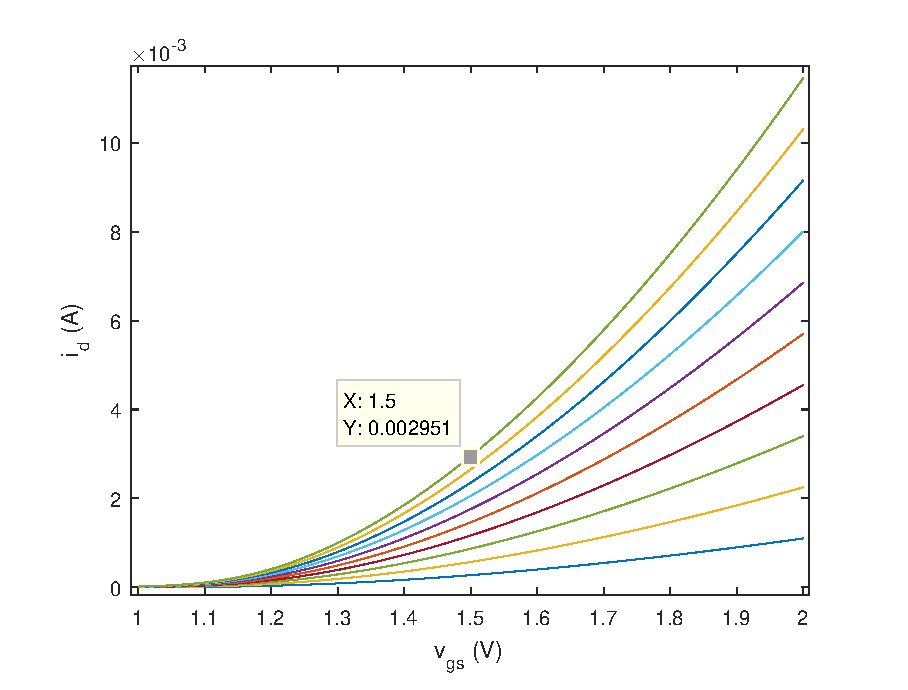
\includegraphics[scale=0.5]{W2_id}
		\caption{I\textsubscript{D3} vs V\textsubscript{GS3} curve. W\textsubscript{3} varying from 50\(\mu\)m to 500\(\mu\)m, $V_{DS3} = 1.5 V$.}
		\label{fig:W_2_id}
	\end{figure}
\end{frame}

\begin{frame}
	\frametitle{Gilbert cell CAD design - Step 1}
	 \begin{columns}[c]
	 \column{0.7\textwidth}
	 \begin{figure}[H]
	 	\centering
	 	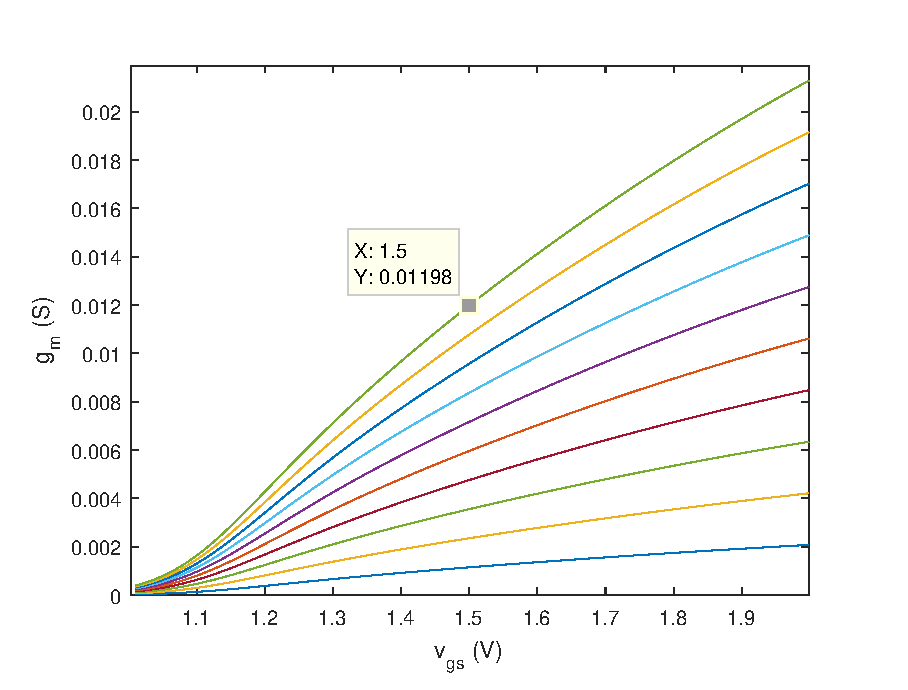
\includegraphics[scale=0.5]{W2_gm}
	 	\caption{g\textsubscript{m3} vs V\textsubscript{GS3} curve. W\textsubscript{3} varying from 50\(\mu\)m to 500\(\mu\)m, $V_{DS3} = 1.5 V$.}
	 	\label{fig:W_2_gm}
	 \end{figure}
 	 \column{0.3\textwidth}
 	 We chose:
 	 \begin{itemize}
 	 	\item $W_3=500\mu $m
 	 	\item $V_{GS3}=1.5 $V
 	 	\item $g_{m3}=11.9$mS
 	 	\item $I_0/2=2.9$mA
 	 \end{itemize}
	 \end{columns}
	
\end{frame}

%new frame
\begin{frame}
\frametitle{Gilbert cell CAD design - Step 2}
\begin{columns}[c]
	\column{0.6\textwidth}
	
	\textbf{Step 2}: design the current sink. We \textbf{have}:
	\begin{itemize} 
		\item voltage on R\textsubscript{S}:
		\begin{gather}
		V_{R_S}=2.9mA\times 10 \Omega =29 mV \notag
		\end{gather}
		\item Voltages on M\textsubscript{1}
		\begin{align}
		V_{DS1} &=1.5 V- V_{R_S} = 1.471V\notag \\
		 V_{GS1} &= 1.471V \notag
		\end{align}
	\end{itemize}
	From simulation we get W\textsubscript{3}=373$\mu m$ to have I\textsubscript{0}=5.8mA.
	
	\column{0.35\textwidth}
	\begin{figure}[H]
		\centering
		\scalebox{0.5}{
			\begin{circuitikz}
				\ctikzset{tripoles/mos style/arrows,bipoles/length=1cm}
				%I_0 and RS
				\draw (0,-1) node[sground]{};
				\draw (0,-1) to[Tnmos,n=M1] (0,0);
				\draw (M1.gate) to[short,-*] (M1.gate);
				\draw (0,0) to[short,i_<=$I_0$] (0,1);
				\draw (0,1) to[short,-] (-0.2,1) to[R,l_=$R_S$] (-2,1) -| (-2.5,2) to[Tnmos,n=M3] (-2.5,3) to[short,-] (-2.5,3.5) to[twoport,l=$LO_{stage}$] (-2.5,4.5);
				\draw (M3.source) node[right=3mm, above=3mm]{$M3$};
				\draw (0,1) to[short,-] (0.2,1) to[R,l=$R_S$] (2,1) -| (2.5,2) to[Tnmos,n=M4,mirror] (2.5,3) to[short,-] (2.5,3.5) to[twoport,l=$LO_{stage}$] (2.5,4.5);
				\draw (M4.source) node[left=3mm, above=3mm]{$M4$};
				\draw (M3.gate) -| (-4,2.5) to[short,-*] (-4,2.5) node[below]{};
				\draw (M4.gate) -| (4,2.5) to[short,-*] (4,2.5) node[below]{};
				%voltage arrows
				\draw (M1.source) to[open, v^=$V_{GS1}$] (M1.gate);
				\draw (-1.5,-1.7) to[open, v^=$V_{SB3}$] (-2.5,1);
				\draw (M3.source) to[open, v^=$V_{GS3}$] (M3.gate);
				\draw (-2,1.7) to[open, v=$V_{DS3}$] (-2,3);
				\draw (0,0.9) to[open, v^=$V_{RS}$] (-2,0.9);
			\end{circuitikz}
		}
		\caption{Gain stage.}
		\label{fig:GainStage}
	\end{figure}
\end{columns}
\end{frame}

\begin{frame}
	\frametitle{Gilbert cell CAD design - Step 2}
	\begin{figure}[H]
		\centering
		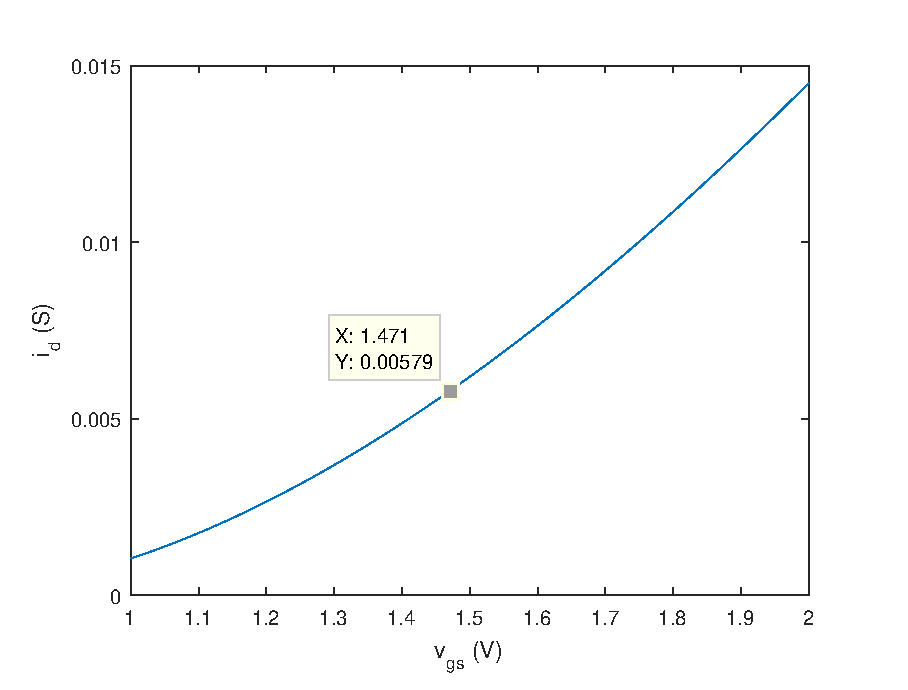
\includegraphics[scale=0.5]{W1_id}
		\caption{I\textsubscript{D1} vs V\textsubscript{GS1} curve. W=\(373\mu m\)}
		\label{W1_id}
	\end{figure}
\end{frame}

%new frame
\begin{frame}
\frametitle{Gilbert cell CAD design - Step 3}
\begin{columns}[c]
	\column{0.65\textwidth}

	\textbf{Step 3}: design the mixing stage. 

	From \textbf{design spec} we have: 
	\begin{align}
	A_v \approx \frac{2}{\pi}\left( \frac{R_L}{R_S + \frac{1}{g_{m3}}}\right)=4 \nonumber
	\end{align}
	therefore
	\begin{align}
	R_L&=A_v \cdot \left( \frac{\pi}{2} \cdot\frac{1}{g_{m3}} + R_S \right)  \notag \\
	&= 4\times \left( \frac{\pi}{2}\times\frac{1}{11.9mS} + 10\Omega \right)=577 \Omega \notag
	\end{align}
	\column{0.35\textwidth}
		\begin{figure}[H]
			\centering
			\scalebox{0.4}{
					\begin{circuitikz}
					\ctikzset{tripoles/mos style/arrows,bipoles/length=1cm}
					
					\draw (-2,4) -- (-3,4)
					to[Tnmos,n=M6] (M6.drain) to[R,l=$R_L$] (-3,7) -- (3,7)
					(M6.source) node[right=3mm, above=3mm]{$M6$};
					
					\draw (-2,4) -- (-1,4) to[Tnmos,mirror,n=M7] (M7.drain) to[R,l=$R_L$] (-1,7)
					(M7.source) node[left=3mm, above=4mm]{$M7$};
					
					\draw (2,4) -- (1,4) to[Tnmos,n=M8] (M8.drain) to[R,l=$R_L$] (1,7)
					(M8.source) node[right=3mm, above=3mm]{$M8$};
					
					\draw (2,4) -- (3,4) to[Tnmos,mirror,n=M9] (M9.drain) to[R,l=$R_L$] (3,7)
					(M9.source) node[left=3mm, above=3mm]{$M9$};
					
					%drawing VLO-
					\draw (M7.gate) -- (M8.gate);
					\draw (M7.gate) -| (0,4) to[short,-*] (0,4);
					
					%Out nodes
					\draw (M6.gate) -| (-5,4.65)  to[short,-*] (-5,4.65);
					\draw (M9.gate) -| (5,4.65)  to[short,-*] (5,4.65);
					\draw (-2,3) -- (-2,4)
					(2,3) -- (2,4);
					\draw (0,7) node[above]{$V_{DD}$};
					\draw (-2,0) node[sground]{} to[open, v^=$V_{SB6}$] (M6.source) to[open, v^=$V_{GS6}$] (M6.gate);
					\draw (-2.5,4) to[open,v=$V_{DS6}$] (-2.5,5);
					\draw (-4,5) to[open,v^=$V_{RL}$] (-4,7);
				\end{circuitikz}
			}
			\caption{Gain stage.}
			\label{fig:GainStage}
		\end{figure}
	\end{columns}
\end{frame}

%new frame
\begin{frame}
	\frametitle{Gilbert cell CAD design - Step 3}
	\begin{columns}[c]
	\column{0.65\textwidth}
	One has:
	\begin{align}
	V_{SB6}&=V_{DS1}+V_{R_S}+V_{DS3} \notag\\
	&= 1.47V+0.029V+1.5V=3V \nonumber
	\end{align}
	hence:
	\begin{align}	
	&V_{R_L}=2.9mA\times 577\Omega=1.673V \nonumber \\
	&V_{DS6}=V_{dd}-V_{R_L}-V_{SB6}=327mV \nonumber
	\end{align}
	We need \emph{switches} slightly above threshold.
	\column{0.35\textwidth}
	\begin{figure}[H]
		\centering
		\scalebox{0.4}{
			\begin{circuitikz}
				\ctikzset{tripoles/mos style/arrows,bipoles/length=1cm}
				
				\draw (-2,4) -- (-3,4)
				to[Tnmos,n=M6] (M6.drain) to[R,l=$R_L$] (-3,7) -- (3,7)
				(M6.source) node[right=3mm, above=3mm]{$M6$};
				
				\draw (-2,4) -- (-1,4) to[Tnmos,mirror,n=M7] (M7.drain) to[R,l=$R_L$] (-1,7)
				(M7.source) node[left=3mm, above=4mm]{$M7$};
				
				\draw (2,4) -- (1,4) to[Tnmos,n=M8] (M8.drain) to[R,l=$R_L$] (1,7)
				(M8.source) node[right=3mm, above=3mm]{$M8$};
				
				\draw (2,4) -- (3,4) to[Tnmos,mirror,n=M9] (M9.drain) to[R,l=$R_L$] (3,7)
				(M9.source) node[left=3mm, above=3mm]{$M9$};
				
				%drawing VLO-
				\draw (M7.gate) -- (M8.gate);
				\draw (M7.gate) -| (0,4) to[short,-*] (0,4);
				
				%Out nodes
				\draw (M6.gate) -| (-5,4.65)  to[short,-*] (-5,4.65);
				\draw (M9.gate) -| (5,4.65)  to[short,-*] (5,4.65);
				\draw (-2,3) -- (-2,4)
				(2,3) -- (2,4);
				\draw (0,7) node[above]{$V_{DD}$};
				\draw (-2,0) node[sground]{} to[open, v^=$V_{SB6}$] (M6.source) to[open, v^=$V_{GS6}$] (M6.gate);
				\draw (-2.5,4) to[open,v=$V_{DS6}$] (-2.5,5);
				\draw (-4,5) to[open,v^=$V_{RL}$] (-4,7);
			\end{circuitikz}
		}
		\caption{Gain stage.}
		\label{fig:GainStage}
	\end{figure}
	\end{columns}
\end{frame}

\begin{frame}
	\frametitle{Gilbert cell CAD design - Step 3}
	\begin{figure}[H]
		\centering
		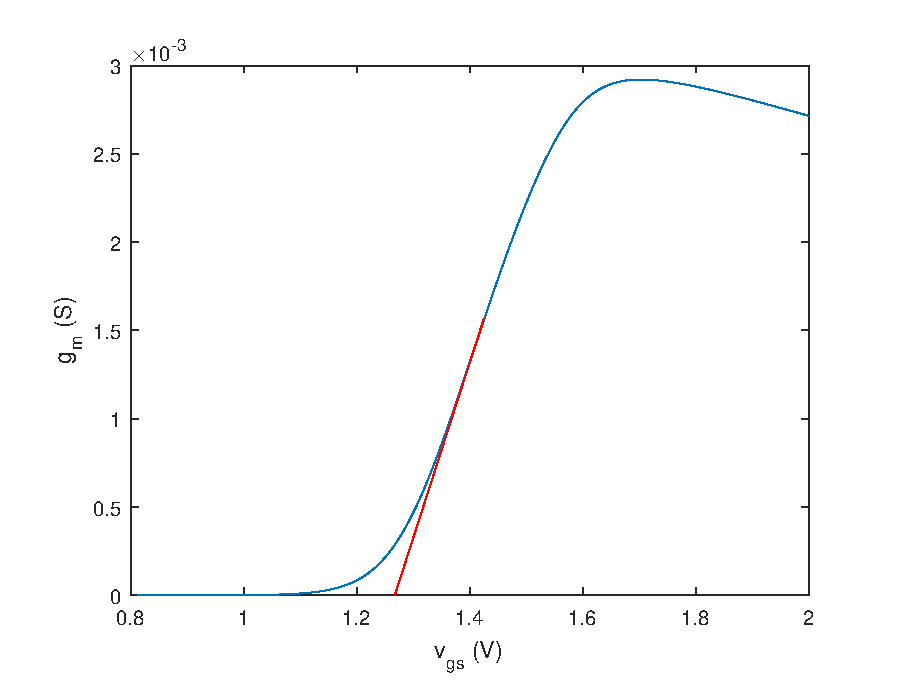
\includegraphics[scale=0.5]{M6_Vth}
		\caption{Extrapolation of M6 threshold voltage from transconductance versus the \(V_{GS}\) curve. The threshold is located at \(1.27V\).}
		\label{M6_Vth}
	\end{figure}
\end{frame}

%new frame
\begin{frame}
\frametitle{Gilbert cell CAD design - Step 3}
	\begin{columns}[c]
	\column{0.65\textwidth}
	From simulation we chose V\textsubscript{od6}=60mV.
	Then:
	\begin{align}
		&V_{GS6}=V_{th6}+ V_{od6}=1.33V \nonumber
	\end{align}
	By characterizing the device:
	\begin{align}
		&W_6=170.3\mu m \nonumber\\
		&L = L_{min} = 0.6\mu m \nonumber
	\end{align} 
	Minimum gate length: fast.
	\column{0.35\textwidth}
	\begin{figure}[H]
		\centering
		\scalebox{0.4}{
			\begin{circuitikz}
				\ctikzset{tripoles/mos style/arrows,bipoles/length=1cm}
				
				\draw (-2,4) -- (-3,4)
				to[Tnmos,n=M6] (M6.drain) to[R,l=$R_L$] (-3,7) -- (3,7)
				(M6.source) node[right=3mm, above=3mm]{$M6$};
				
				\draw (-2,4) -- (-1,4) to[Tnmos,mirror,n=M7] (M7.drain) to[R,l=$R_L$] (-1,7)
				(M7.source) node[left=3mm, above=4mm]{$M7$};
				
				\draw (2,4) -- (1,4) to[Tnmos,n=M8] (M8.drain) to[R,l=$R_L$] (1,7)
				(M8.source) node[right=3mm, above=3mm]{$M8$};
				
				\draw (2,4) -- (3,4) to[Tnmos,mirror,n=M9] (M9.drain) to[R,l=$R_L$] (3,7)
				(M9.source) node[left=3mm, above=3mm]{$M9$};
				
				%drawing VLO-
				\draw (M7.gate) -- (M8.gate);
				\draw (M7.gate) -| (0,4) to[short,-*] (0,4);
				
				%Out nodes
				\draw (M6.gate) -| (-5,4.65)  to[short,-*] (-5,4.65);
				\draw (M9.gate) -| (5,4.65)  to[short,-*] (5,4.65);
				\draw (-2,3) -- (-2,4)
				(2,3) -- (2,4);
				\draw (0,7) node[above]{$V_{DD}$};
				\draw (-2,0) node[sground]{} to[open, v^=$V_{SB6}$] (M6.source) to[open, v^=$V_{GS6}$] (M6.gate);
				\draw (-2.5,4) to[open,v=$V_{DS6}$] (-2.5,5);
				\draw (-4,5) to[open,v^=$V_{RL}$] (-4,7);
			\end{circuitikz}
		}
		\caption{Gain stage.}
		\label{fig:GainStage}
	\end{figure}
	\end{columns}
\end{frame}

\begin{frame}
	\frametitle{Bias net design - M\textsubscript{5} }
	\begin{columns}
		\column{0.65\textwidth}
		Now the bias net is designed. From \textbf{spec}:
		\begin{align}                                                             V_{G1}&=1.471 V \nonumber \\  
		V_{G3}&=3 V \nonumber \\
		V_{G6}&=4.33 V \nonumber
		\end{align} 
		We chose mirroring ratio 1:1, $L_2=1.8\mu m$ (same length of M\textsubscript{1}) and \(V_{GS2}=V_{DS2}=1.471V\). To have I\textsubscript{0}=5.8mA from \textbf{simulation}:
		\begin{align}
			&W_2=373\mu m \notag
		\end{align}
		Since $V_{G5}=3V$, from \textbf{simulation}:
		\begin{align}
		&W_5=130.45\mu m \nonumber\\
		&L_5=0.6\mu m \nonumber
		\end{align}  
		\column{0.35\textwidth}
		\begin{figure} [H]
			\centering
			\scalebox{0.6}{
			\begin{circuitikz}
				\ctikzset{tripoles/mos style/arrows,bipoles/length=1cm}
				\ctikzset{bipoles/capacitor/height=0.5}
				\ctikzset{bipoles/capacitor/width=0.1}
				%M2
				\draw (0,0) to[Tnmos,mirror,n=M2] (0,2);
				\draw (M2.source) node[left=3mm,above=3mm]{$M2$};
				\draw (M2.gate)[right] |- (M2.drain);
				\draw (M2.gate) to[short,-*] (2.5,1) node[right]{to $G_1$};
				\draw (M2.source) to[short] (0,0) node[sground]{};
				\draw (0,6) -- (-2,6) to[C=$C_{1}$] (-2,5) node[sground]{};
				%M5
				\draw (M2.drain) to[Tnmos,mirror,n=M5] (0,4.5);
				\draw (M5.source) node[left=3mm,above=3mm]{$M5$};
				\draw (M5.gate)[right] |- (M5.drain);
				\draw (0,4) -- (-2,4) to[C=$C_{2}$] (-2,3) node[sground]{};
				\draw (M5.gate) to[R, l_=$R_1$] (2,2.3) to[short,-*] (2.5,2.3) node[right]{to $G_3$};
				\draw (M5.gate) to[R=$R_1$] (2,3.7) to[short,-*] (2.5,3.7) node[right]{to $G_4$};
				%R2 R4
				\draw (M5.drain) to[R=$R_2$,n=R2] (0,6.3) to[R=$R_4$] (0,7.1) to[short,-*] (0,7.5) node[above]{$V_{dd}$};
				\draw (0,5.7) to[short] (0.7,5.7) to[R,l_=$R_3$] (2,5) to[short,-*] (2.5,5) node[right]{to $G_6$,$G_9$};
				\draw (0,5.7) to[short] (0.7,5.7) to[R=$R_3$] (2,6.4) to[short,-*] (2.5,6.4) node[right]{to $G_7$,$G_8$};
			\end{circuitikz}
			}
			\caption{Reference biasing network schematic}
			\label{fig:biasNet1}
		\end{figure}
	\end{columns}	
\end{frame}

\begin{frame}
	\frametitle{Bias net design - R\textsubscript{2},R\textsubscript{4}}
	\begin{columns}
	\column{0.65\textwidth}
	Voltage drop on R\textsubscript{2} and R\textsubscript{4}:
	\begin{align}
		&R_2+R_4=\frac{V_{dd}-V_{G5}}{I_0} = 344\Omega\nonumber
	\end{align}
	Since $V_{G6}=4.33V$:
	\begin{align}
		&R_2=229\Omega \nonumber\\
		&R_4=115\Omega \nonumber
	\end{align}	
	
	Total \textbf{static power consumption} is $P = 2\times(5.8mA \times 5V) = 58mW$
	\column{0.35\textwidth}
	\begin{figure} [H]
		\centering
		\scalebox{0.6}{
			\begin{circuitikz}
				\ctikzset{tripoles/mos style/arrows,bipoles/length=1cm}
				\ctikzset{bipoles/capacitor/height=0.5}
				\ctikzset{bipoles/capacitor/width=0.1}
				%M2
				\draw (0,0) to[Tnmos,mirror,n=M2] (0,2);
				\draw (M2.source) node[left=3mm,above=3mm]{$M2$};
				\draw (M2.gate)[right] |- (M2.drain);
				\draw (M2.gate) to[short,-*] (2.5,1) node[right]{to $G_1$};
				\draw (M2.source) to[short] (0,0) node[sground]{};
				\draw (0,6) -- (-2,6) to[C=$C_{1}$] (-2,5) node[sground]{};
				%M5
				\draw (M2.drain) to[Tnmos,mirror,n=M5] (0,4.5);
				\draw (M5.source) node[left=3mm,above=3mm]{$M5$};
				\draw (M5.gate)[right] |- (M5.drain);
				\draw (0,4) -- (-2,4) to[C=$C_{2}$] (-2,3) node[sground]{};
				\draw (M5.gate) to[R, l_=$R_1$] (2,2.3) to[short,-*] (2.5,2.3) node[right]{to $G_3$};
				\draw (M5.gate) to[R=$R_1$] (2,3.7) to[short,-*] (2.5,3.7) node[right]{to $G_4$};
				%R2 R4
				\draw (M5.drain) to[R=$R_2$,n=R2] (0,6.3) to[R=$R_4$] (0,7.1) to[short,-*] (0,7.5) node[above]{$V_{dd}$};
				\draw (0,5.7) to[short] (0.7,5.7) to[R,l_=$R_3$] (2,5) to[short,-*] (2.5,5) node[right]{to $G_6$,$G_9$};
				\draw (0,5.7) to[short] (0.7,5.7) to[R=$R_3$] (2,6.4) to[short,-*] (2.5,6.4) node[right]{to $G_7$,$G_8$};
			\end{circuitikz}
		}
		\caption{Reference biasing network schematic}
		\label{fig:biasNet1}
	\end{figure}
	\end{columns}	
\end{frame}

\begin{frame}
	\frametitle{Bias net design - R\textsubscript{1,3} and C\textsubscript{1,2} }
	\begin{columns}
	\column{0.65\textwidth}
	Resistors R\textsubscript{1} and R\textsubscript{3} act as AC block:
	\begin{align}
	&R_1=R_3=30k\Omega \nonumber
	\end{align}
	Equivalent resistance seen from C\textsubscript{1}:
	\begin{align}
	R_{eq}\simeq R_2||R4||\frac{R_3}{2}=76.4 \Omega \nonumber
	\end{align}
	Pole frequency un decade before f\textsubscript{LO}:
	\begin{align}
		C_{1}\ge 10\cdot \frac{1}{2\pi \cdot R_{eq} \cdot \frac{f_{lo}}{10}} = 20.8pF \notag
	\end{align}
	From \textbf{optimization}: $C_1=C_2=25pF$.
	\column{0.35\textwidth}
	\begin{figure} [H]
		\centering
		\scalebox{0.6}{
			\begin{circuitikz}
				\ctikzset{tripoles/mos style/arrows,bipoles/length=1cm}
				\ctikzset{bipoles/capacitor/height=0.5}
				\ctikzset{bipoles/capacitor/width=0.1}
				%M2
				\draw (0,0) to[Tnmos,mirror,n=M2] (0,2);
				\draw (M2.source) node[left=3mm,above=3mm]{$M2$};
				\draw (M2.gate)[right] |- (M2.drain);
				\draw (M2.gate) to[short,-*] (2.5,1) node[right]{to $G_1$};
				\draw (M2.source) to[short] (0,0) node[sground]{};
				\draw (0,6) -- (-2,6) to[C=$C_{1}$] (-2,5) node[sground]{};
				%M5
				\draw (M2.drain) to[Tnmos,mirror,n=M5] (0,4.5);
				\draw (M5.source) node[left=3mm,above=3mm]{$M5$};
				\draw (M5.gate)[right] |- (M5.drain);
				\draw (0,4) -- (-2,4) to[C=$C_{2}$] (-2,3) node[sground]{};
				\draw (M5.gate) to[R, l_=$R_1$] (2,2.3) to[short,-*] (2.5,2.3) node[right]{to $G_3$};
				\draw (M5.gate) to[R=$R_1$] (2,3.7) to[short,-*] (2.5,3.7) node[right]{to $G_4$};
				%R2 R4
				\draw (M5.drain) to[R=$R_2$,n=R2] (0,6.3) to[R=$R_4$] (0,7.1) to[short,-*] (0,7.5) node[above]{$V_{dd}$};
				\draw (0,5.7) to[short] (0.7,5.7) to[R,l_=$R_3$] (2,5) to[short,-*] (2.5,5) node[right]{to $G_6$,$G_9$};
				\draw (0,5.7) to[short] (0.7,5.7) to[R=$R_3$] (2,6.4) to[short,-*] (2.5,6.4) node[right]{to $G_7$,$G_8$};
			\end{circuitikz}
		}
		\caption{Reference biasing network schematic}
		\label{fig:biasNet1}
	\end{figure}
	\end{columns}	
\end{frame}

\begin{frame}
	\frametitle{Design CAD validation - Full circuit}
	\begin{figure}[H]
		\centering
		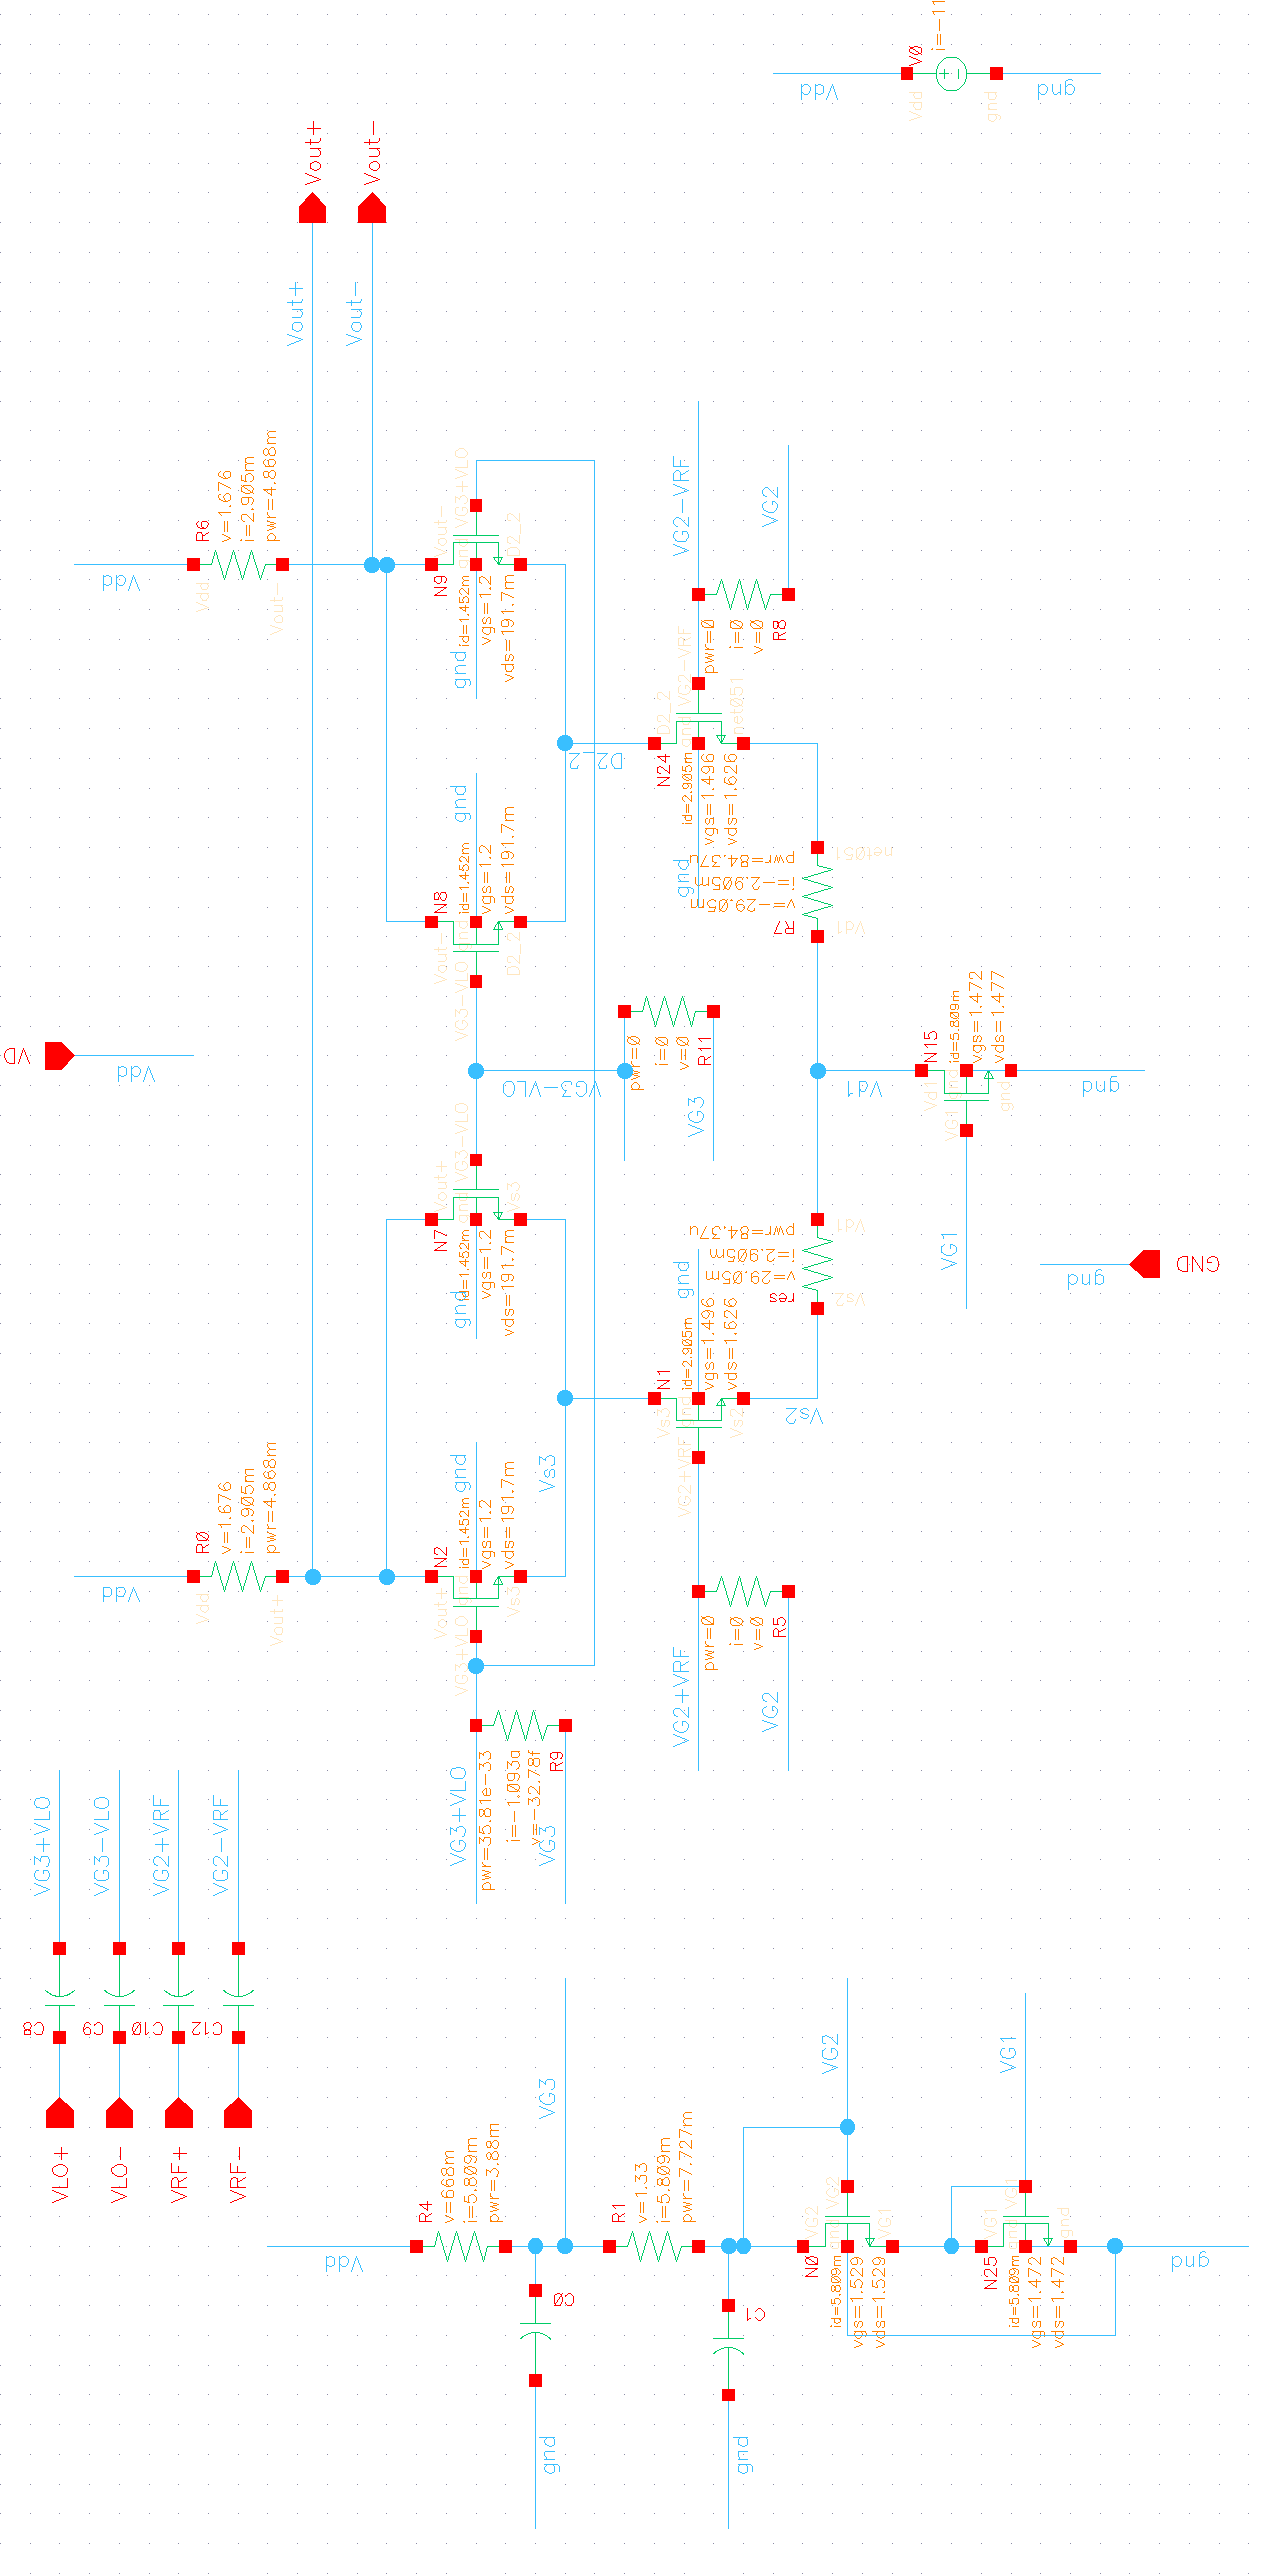
\includegraphics[width=0.5\textwidth, angle=-90]{S_cad_full}
		\caption{Gilbert cell and bias network schematic}
		\label{S_cad_full}
	\end{figure}
\end{frame}

\begin{frame}
	\frametitle{Design CAD validation - Gain stage}
	\begin{figure}[H]
		\centering
		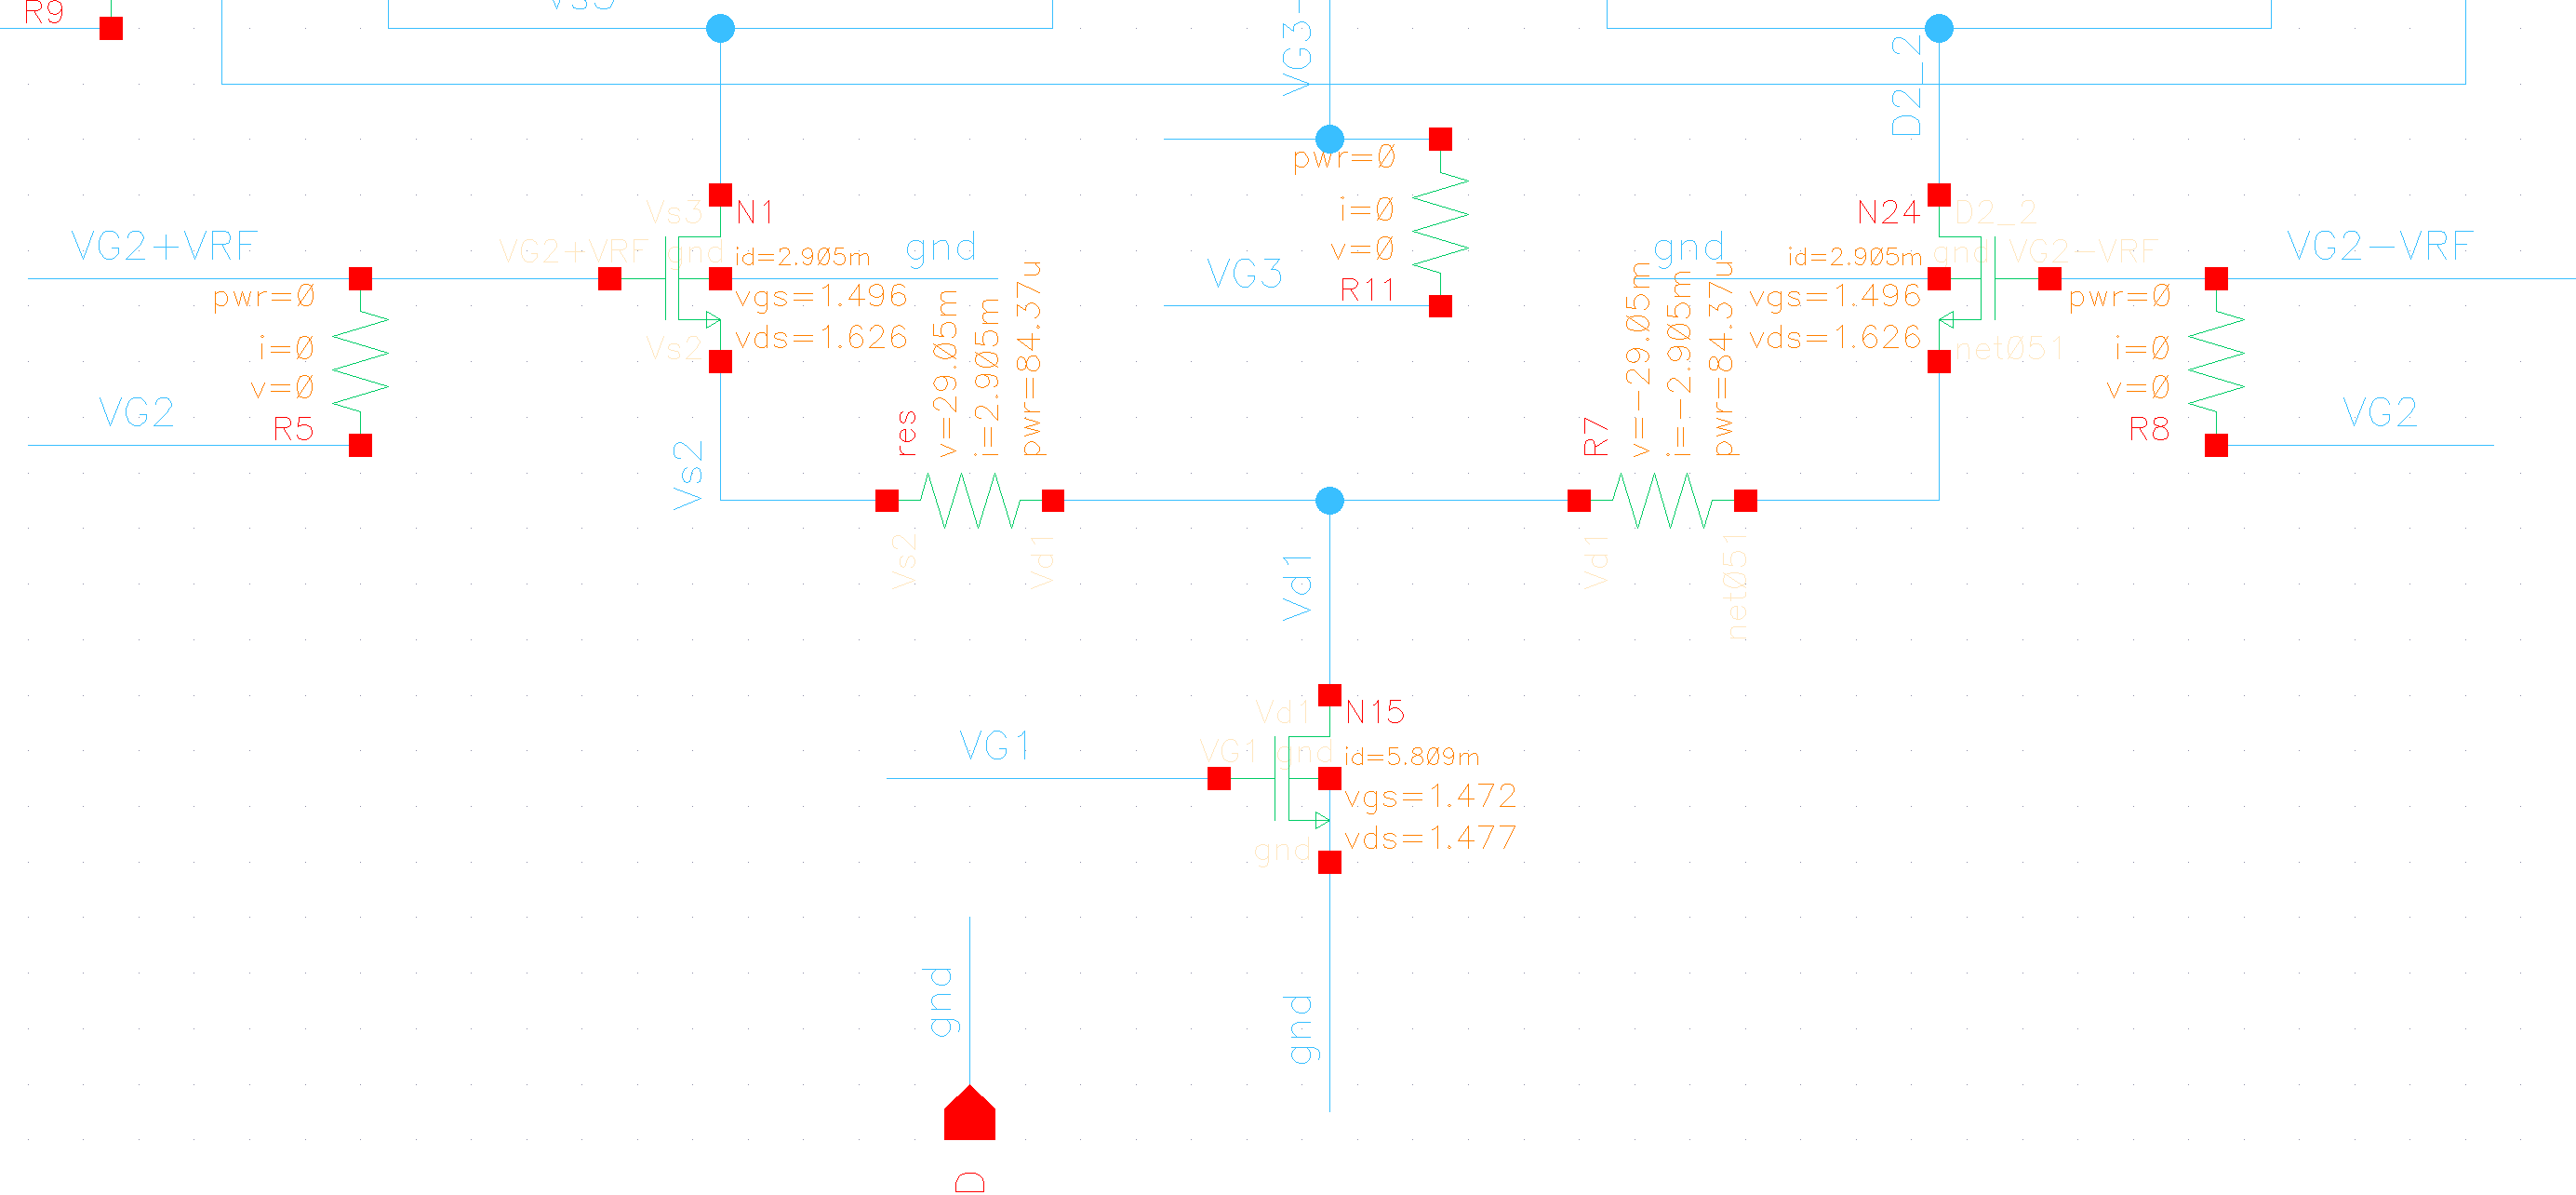
\includegraphics[width=\textwidth]{S_cad_I0}
		\caption{Close up view on current sink and RF stage}
		\label{S_cad_I0}
	\end{figure}
\end{frame}

\begin{frame}
	\frametitle{Design CAD validation - Mixing stage}
	\begin{figure}[H]
	\centering
	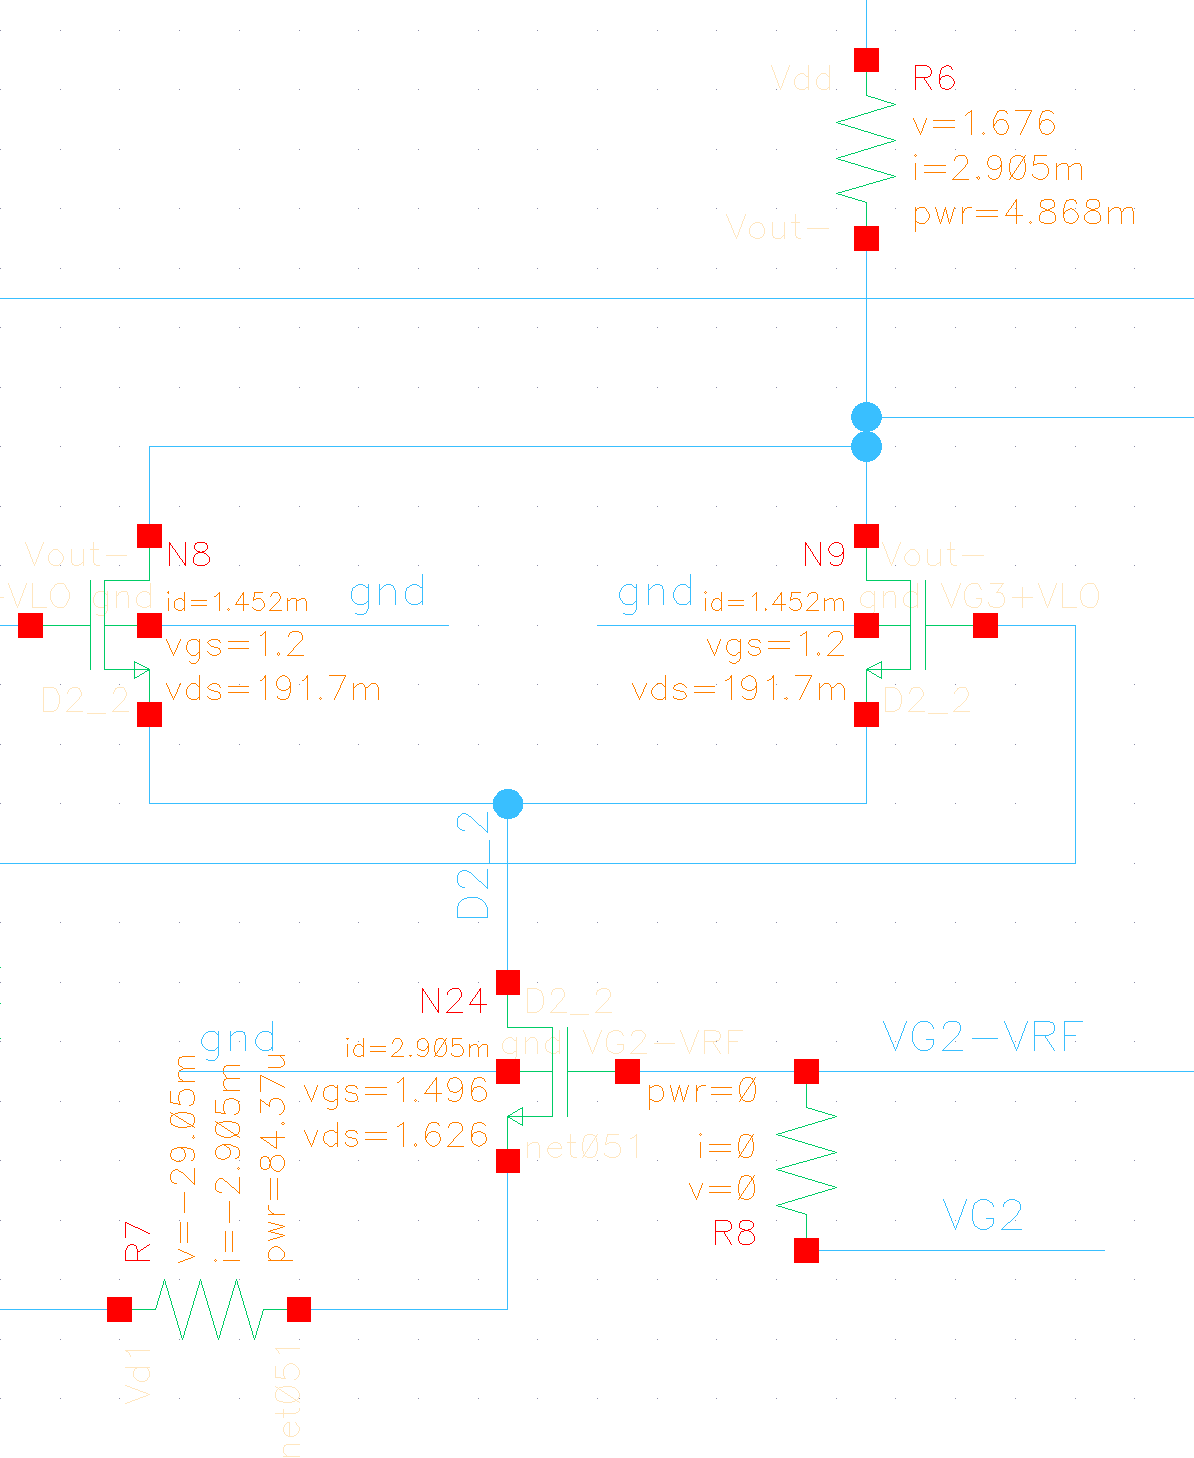
\includegraphics[scale=0.13]{S_cad_LO}
	\caption{Close up view of LO stage\label{subfig-1:S_cad_LO}}
	\label{S_cad_I0}
	\end{figure}
\end{frame}

\begin{frame}
	\frametitle{Design CAD validation - Bias net }
	\begin{figure}[H]
	\centering
	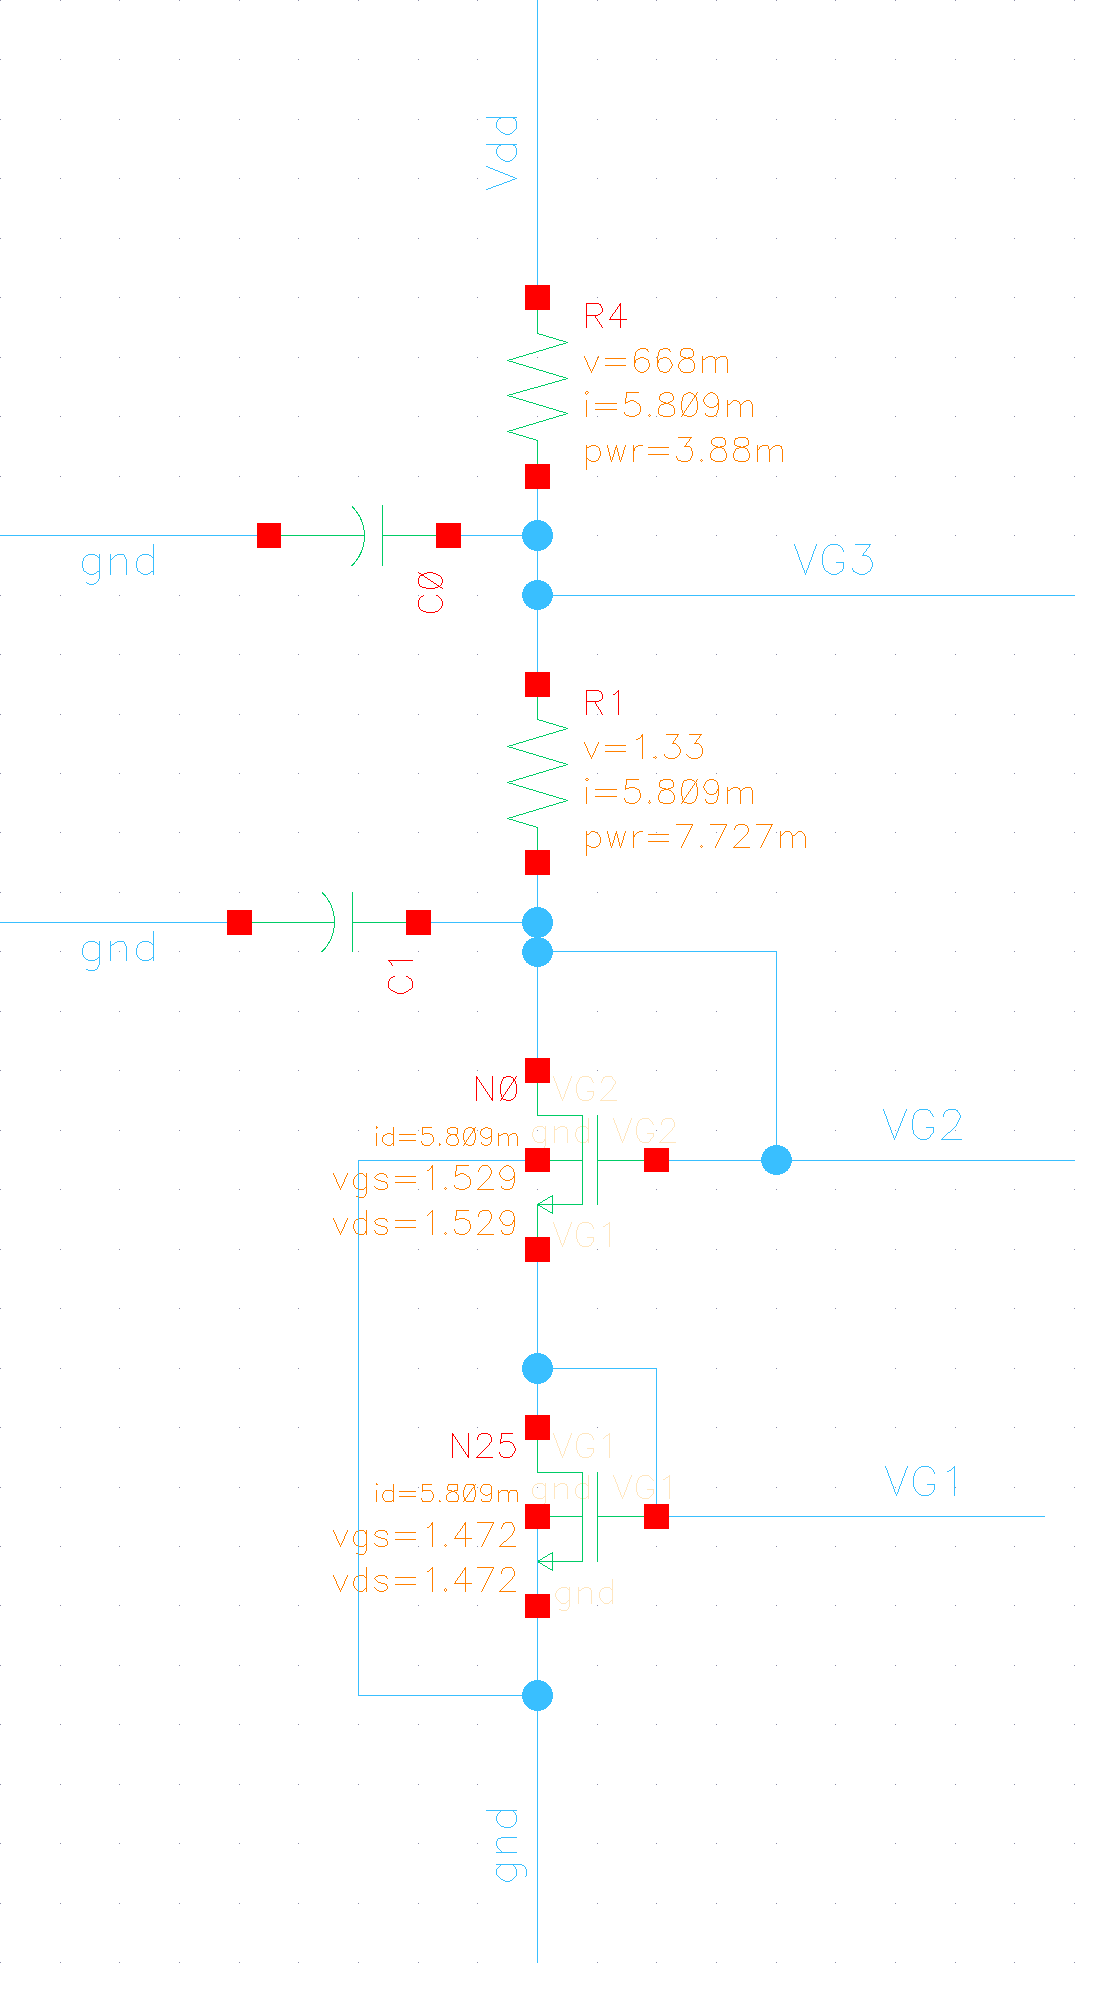
\includegraphics[scale=0.10]{S_cad_biasnet}
	\caption{Close up view of LO stage\label{subfig-1:S_cad_biasnet}}
	\label{S_cad_I0}
	\end{figure}
\end{frame}

\subsection{Layout of the Gilbert cell}
\begin{frame}
	\tableofcontents[currentsubsection]
\end{frame}

\begin{frame}
	\frametitle{Layout strategy}
	\begin{itemize}
		\item Common centroid, interdigitated structures: less gradients;
		\item Multi-finger structure with same-length for transistors fingers: minimize encroachment;
		\item Components with same alignment: uniform error distribution;
		\item Dummy elements: less border effects;
		\item Limited substrate noise with guard rings;
		\item Minimum number of crossed connections and metal changes in the routing process (less parasitics);
		\item Compact and symmetric structure;
		\item Multiple substrate contacts and isolating well used because of circuit width and shared body contact for each MOSFET: less substrate currents.
		\item \textbf{Every device has been optimized} to have matching between circuit and layout.  
	\end{itemize}
\end{frame}

\begin{frame}
	\frametitle{Layout - Gain and Mixing stage}
	\begin{columns}
		\column{0.6\textwidth}
		\begin{itemize}
		\item A \textbf{symmetric} input low noise differential stage is desired.
		\item A common centroid structure is employed along with dummy elements (shorted drain and source).
		\item Same approach with mixing stage: designed to be easily stacked above RF stage, with the two witching stages kept close to each other.
		\end{itemize}
		\column{0.4\textwidth}
		\begin{figure}[H]
			\centering
			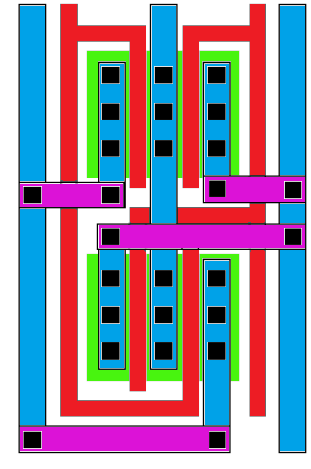
\includegraphics[scale=0.3]{diff_CC}
			\caption{Common centroid structure used for differential RF stage}
			\label{fig:diff_CC}
		\end{figure}
	\end{columns}
\end{frame}

\begin{frame}
	\frametitle{Layout - Gain stage}
	\begin{columns}
		\column{0.3\textwidth}
		M\textsubscript{3,4} parameters:
			\begin{itemize}
				\item m = 18(+2)
				\item w$^*$=34.35$\mu$m
				\item W = 618.3$\mu$m (vs 500$\mu$m)
				\item L = 1.8$\mu$m
				\item y = 126$\mu$m
				\item x = 99.45$\mu$m
			\end{itemize}
		\column{0.7\textwidth}
		\begin{figure}[H]
			\centering
			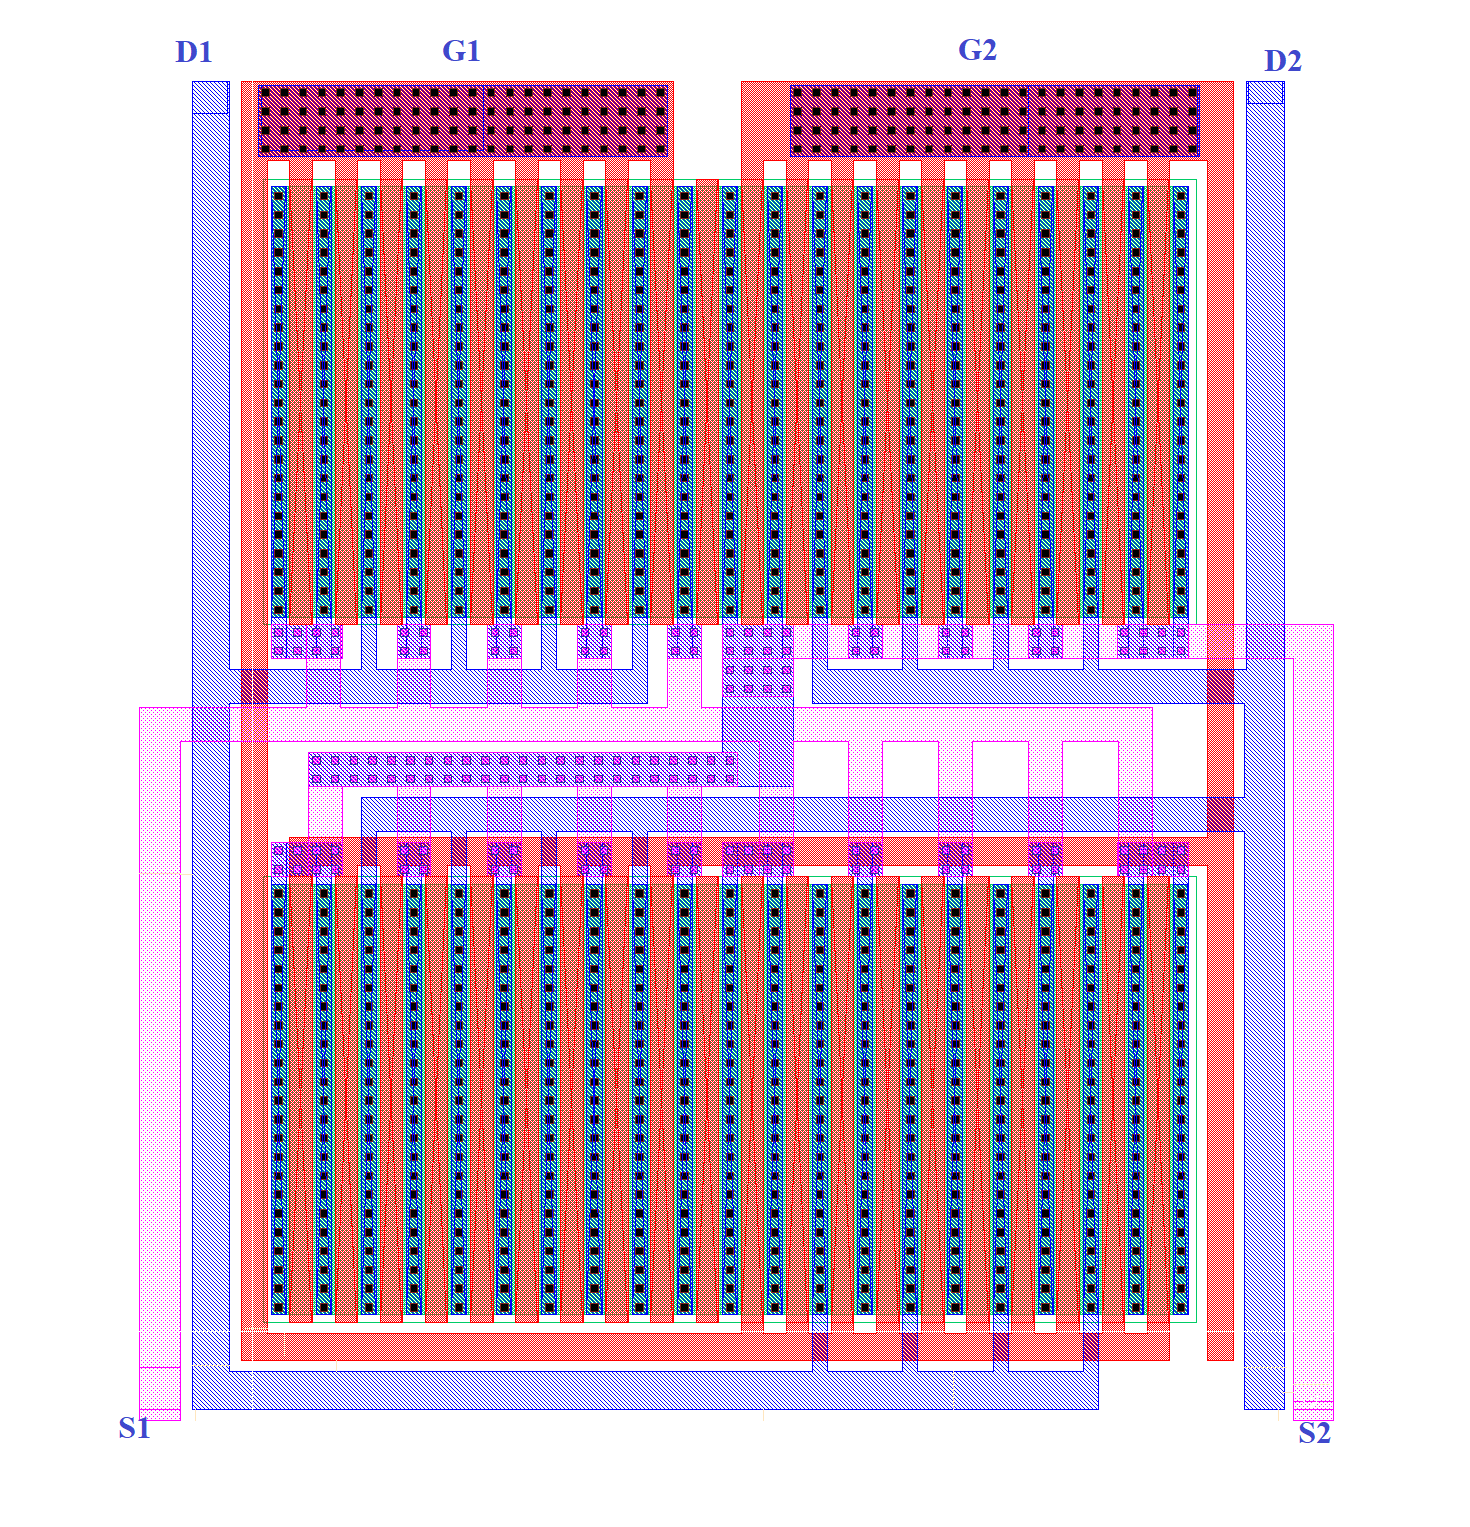
\includegraphics[scale=0.19]{L_RF_full}
			\label{L_RF_full}
		\end{figure}
	\end{columns}
\end{frame}


\begin{frame}
\frametitle{Layout - Mixing stage}
	\begin{columns}
	\column{0.3\textwidth}
	M\textsubscript{6,7,8,9} parameters:
	\begin{itemize}
		\item m = 12(+2)
		\item w$^*$=17.55$\mu$m
		\item W = 210.6$\mu$m (vs 170.3$\mu$m)
		\item L = 0.6$\mu$m
		\item y = 56.85$\mu$m
		\item x = 87.6$\mu$m
	\end{itemize}
	\column{0.7\textwidth}
	\begin{figure}[H]
		\centering
		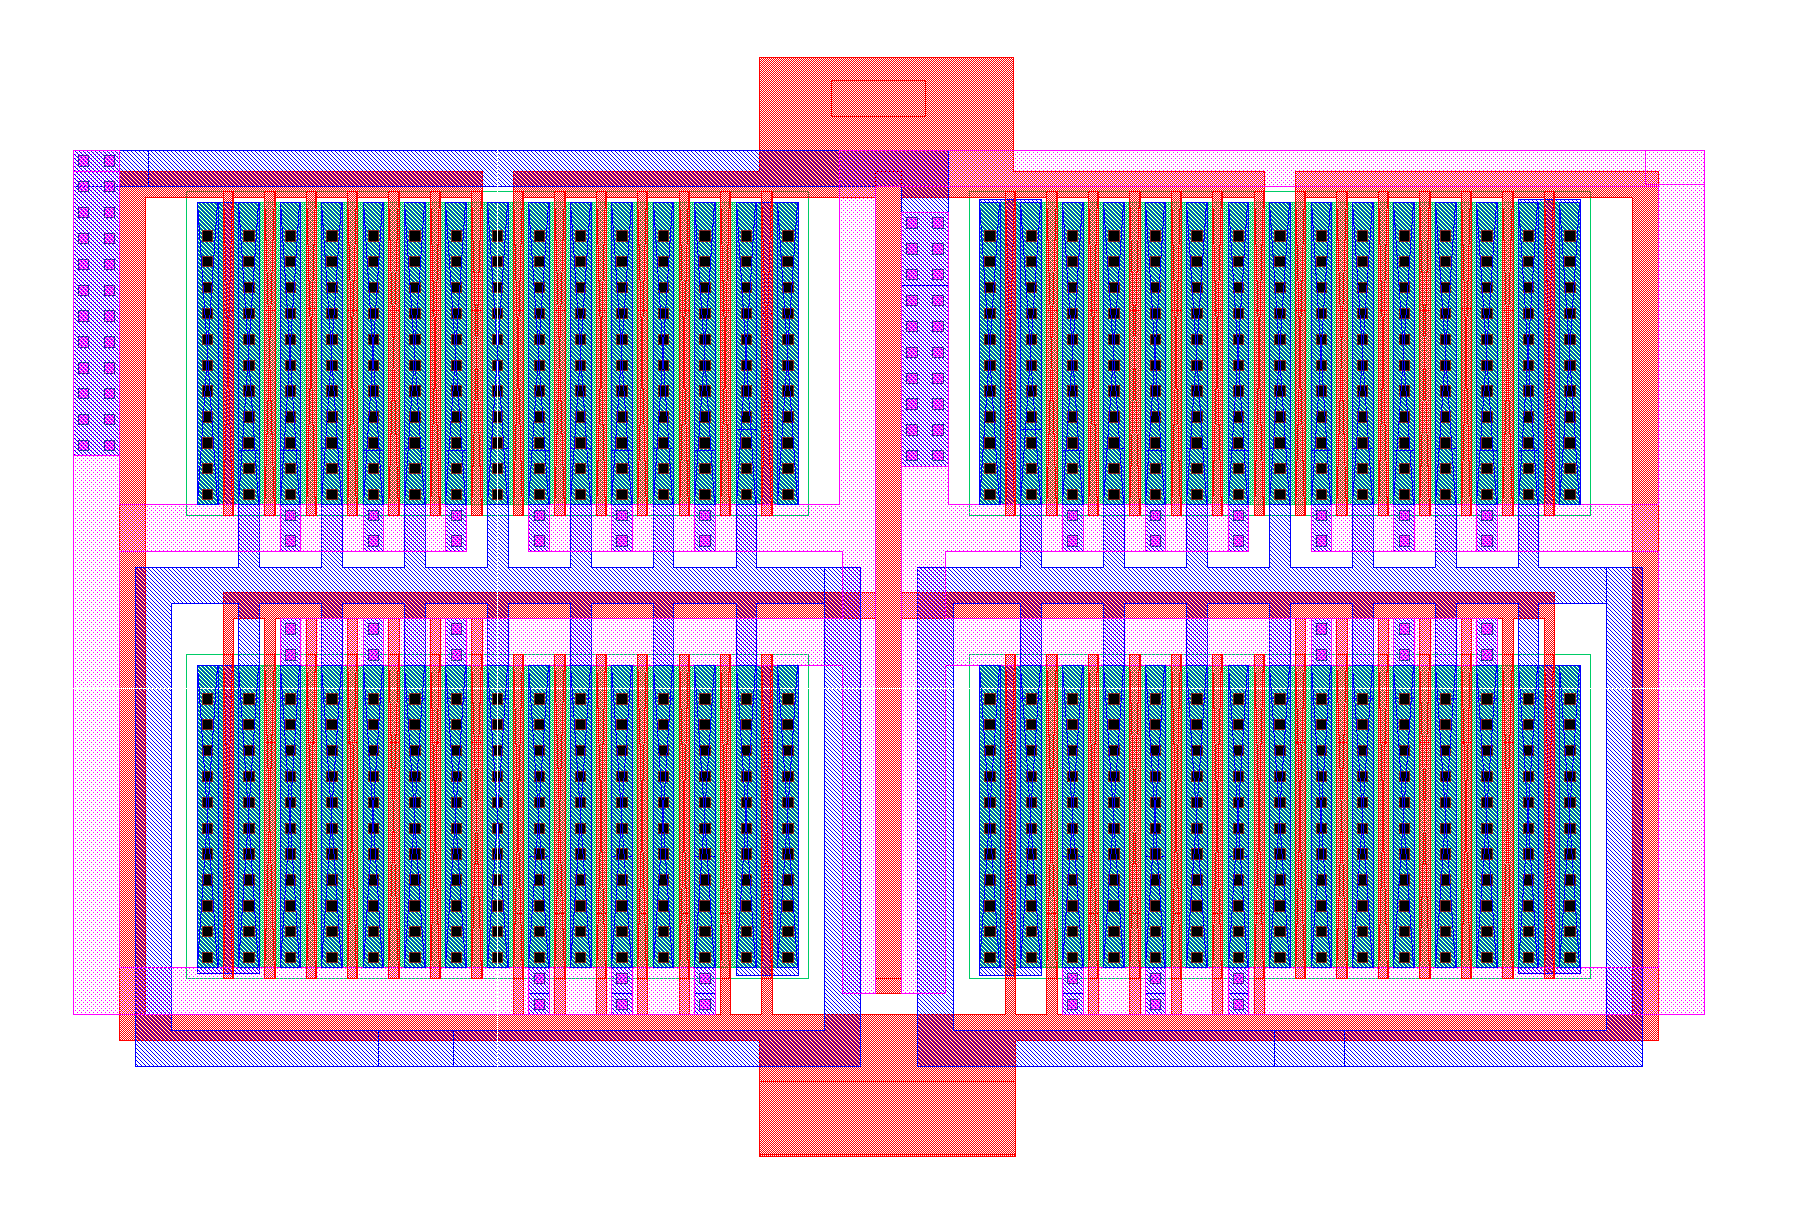
\includegraphics[width=\textwidth]{L_LO_full}
		\label{L_LO_full}
	\end{figure}
	\end{columns}
\end{frame}

\begin{frame}
	\frametitle{Layout - Current mirror}
	\begin{columns}
		\column{0.4\textwidth}
		Current mirror shows multifinger interdigitated structure with dummy elements. M\textsubscript{1,2} parameters:
		\begin{itemize}
			\item m = 10(+1)
			\item w$^*$=39.15$\mu$m
			\item W = 391.15$\mu$m (vs 373$\mu$m)
			\item L = 1.8$\mu$m
			\item y = 61.5$\mu$m
			\item x = 87.75$\mu$m
		\end{itemize}
		\column{0.6\textwidth}
		\begin{figure}[H]
			\centering
			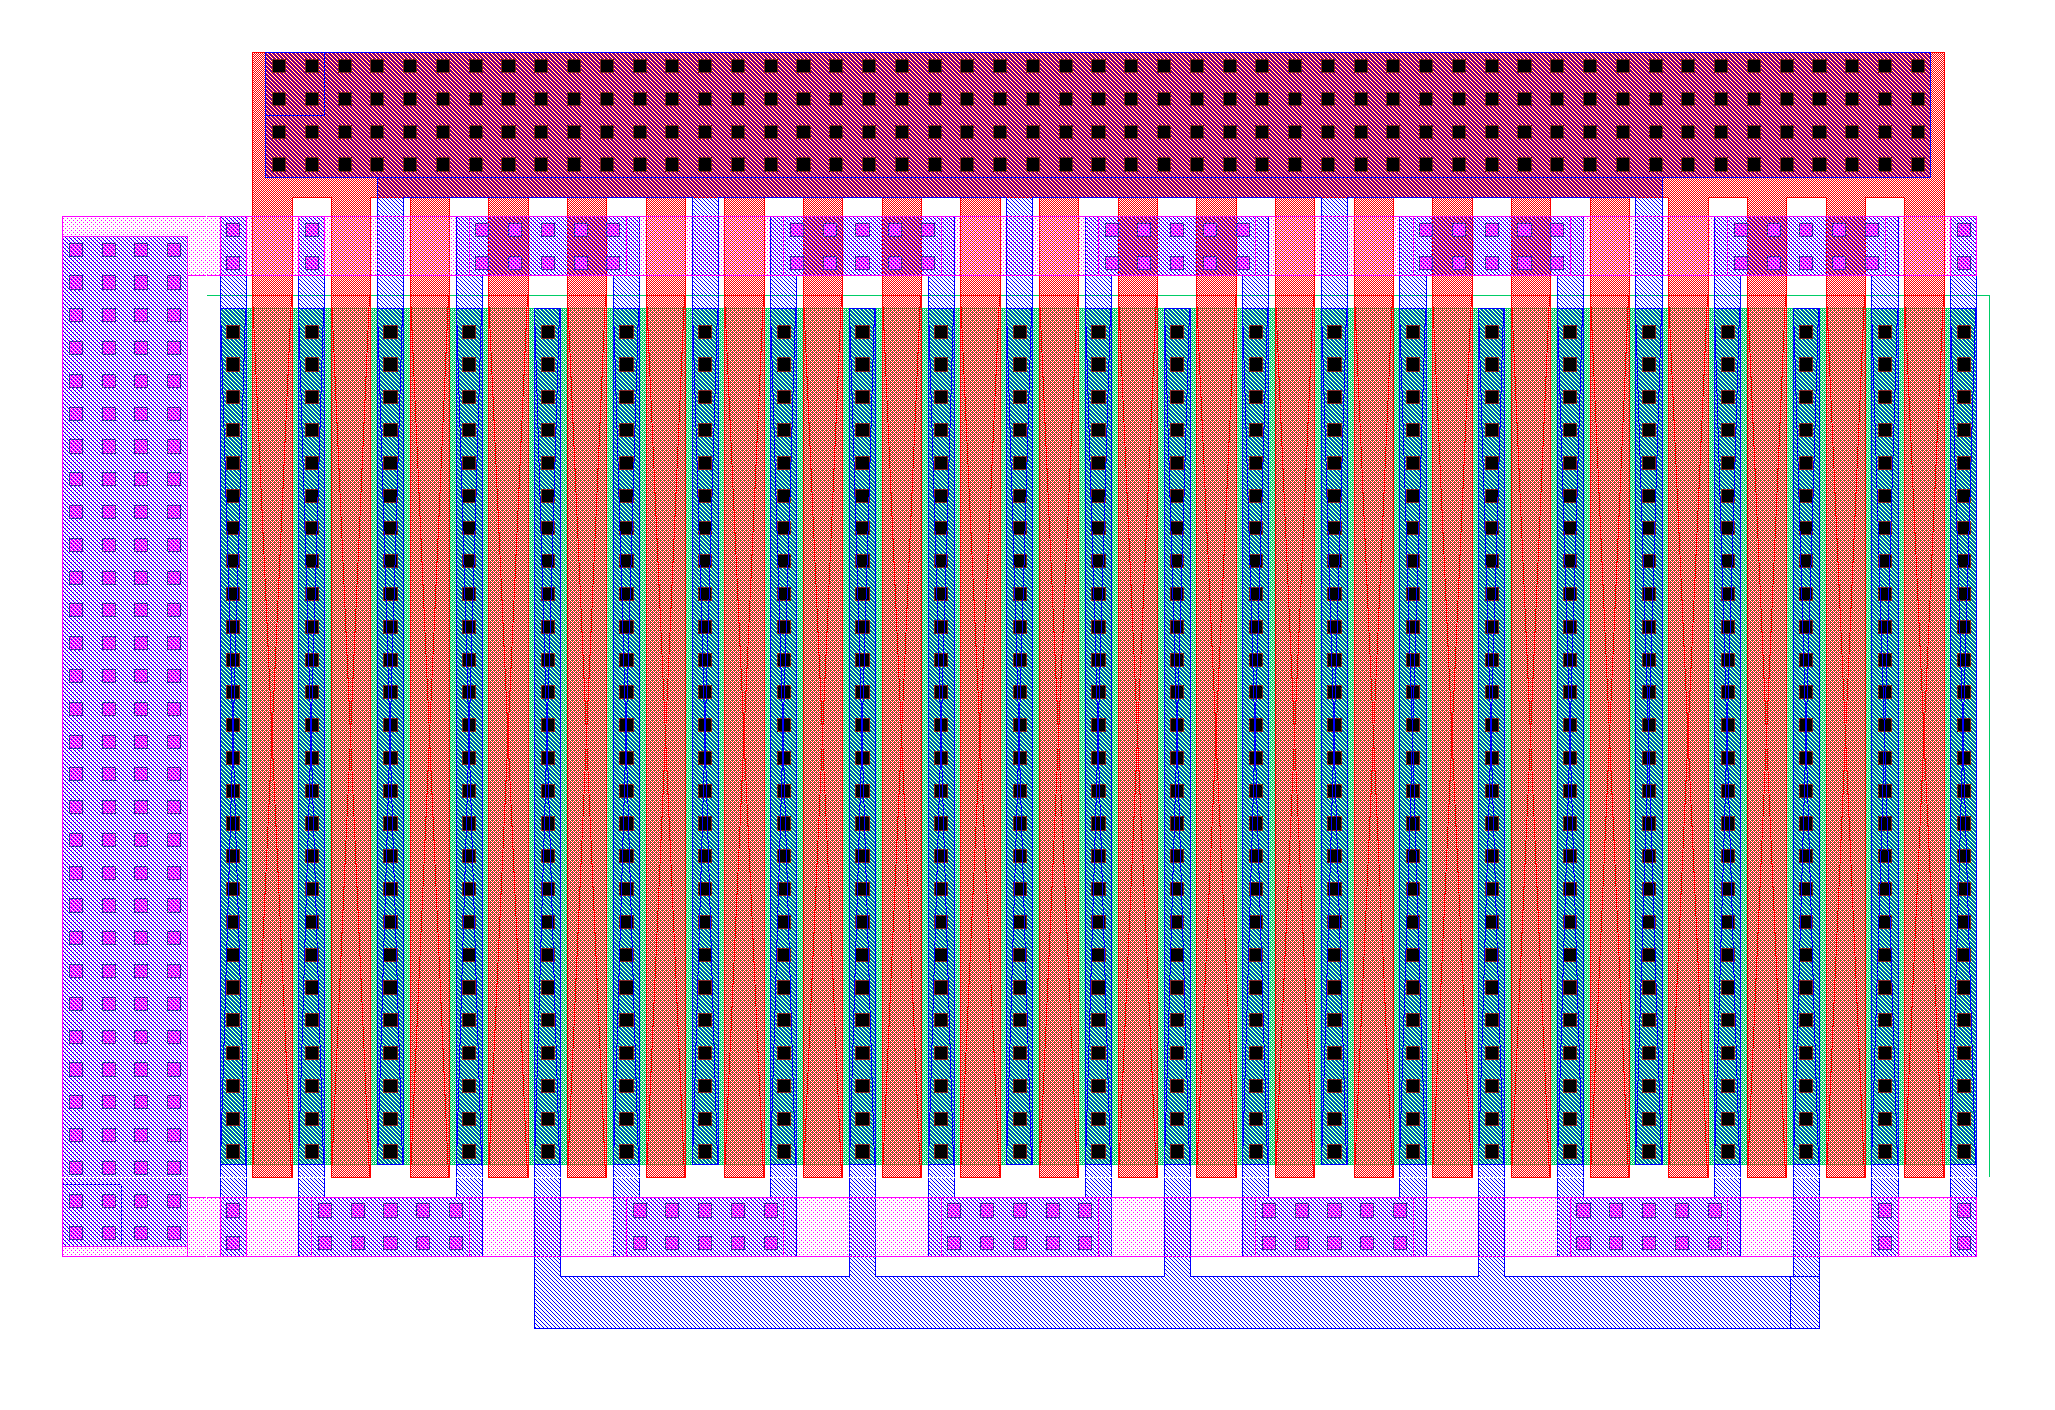
\includegraphics[width=\textwidth]{L_curmir_full}
			\label{L_curmir_full}
		\end{figure}
	\end{columns}
\end{frame}

\begin{frame}
	\frametitle{Layout - M\textsubscript{5}}
	\begin{columns}
		\column{0.4\textwidth}
		M\textsubscript{5} shows multifinger interdigitated structure with dummy 	elements. M\textsubscript{5} parameters:
		\begin{itemize}
			\item m = 12(+2)
			\item w$^*$=13.65$\mu$m
			\item W = 163.8$\mu$m (vs 130.45$\mu$m)
			\item L = 1.8$\mu$m
			\item y = 25.2$\mu$m
			\item x = 35.55$\mu$m
		\end{itemize}
		\column{0.6\textwidth}
		\begin{figure}[H]
			\centering
			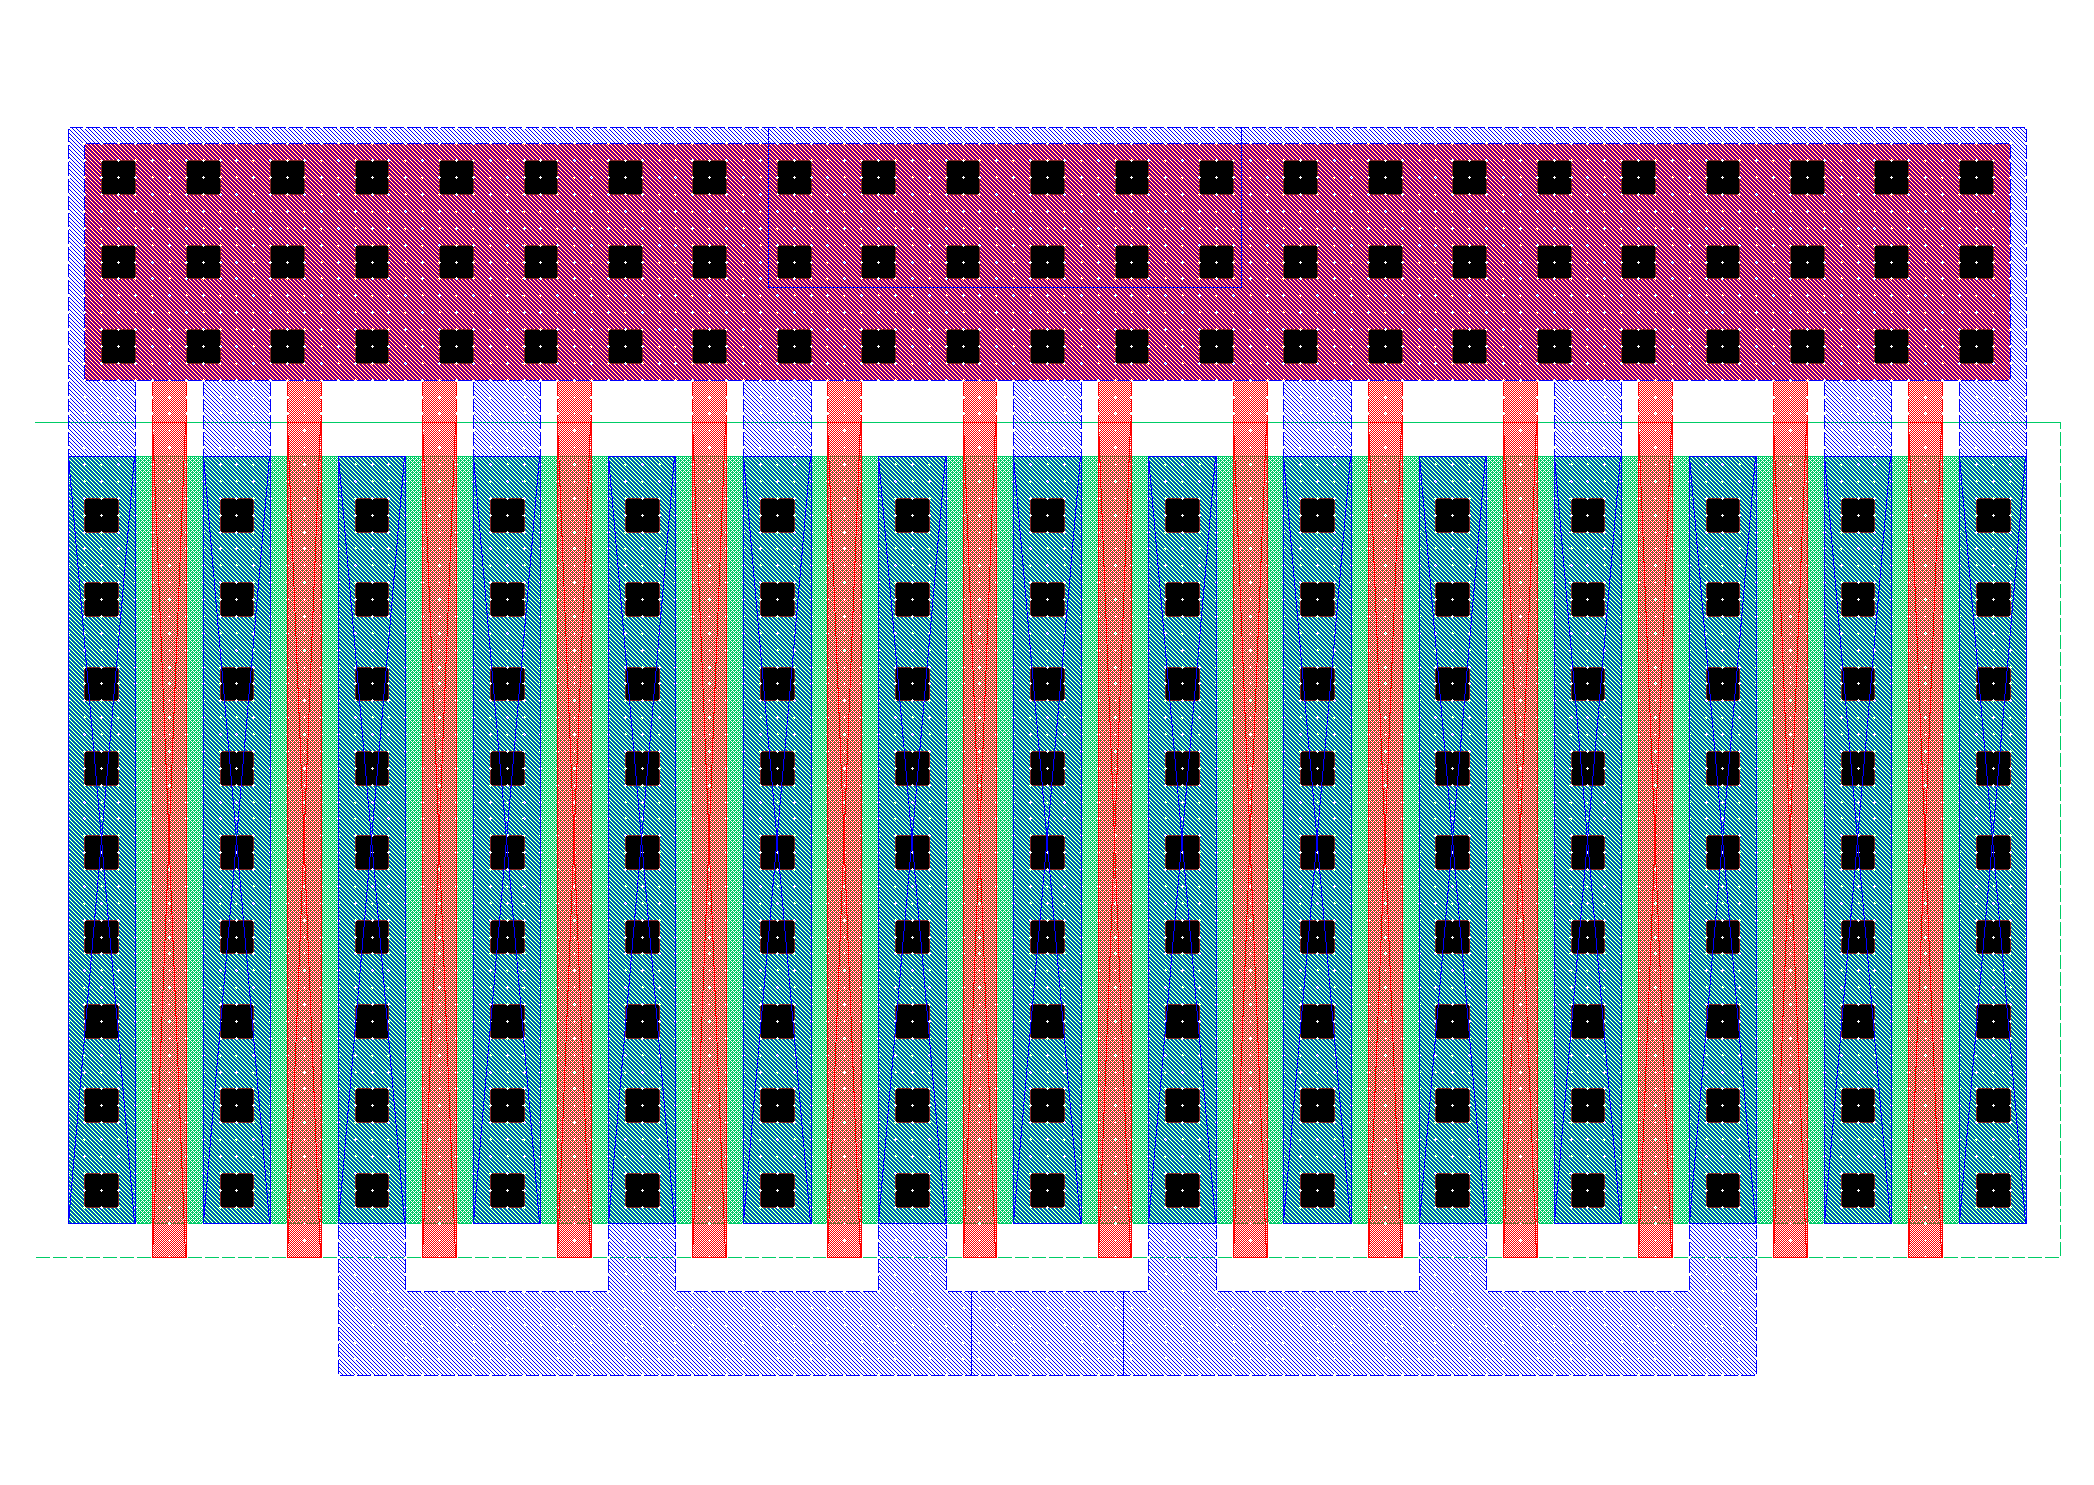
\includegraphics[width=0.8\textwidth]{L_M5_full}
			\label{L_M5_full}
		\end{figure}
	\end{columns}
\end{frame}

\begin{frame}
\frametitle{Layout - C\textsubscript{bias}}
\begin{columns}
	\column{0.6\textwidth}
	\begin{itemize}
		\item C\textsubscript{1,2} are poly capacitors (poly1 + elec) in order to reduce dimensions and improve tolerances. 
		\item Common centroid layout inside n-well (connected to V\textsubscript{DD}) to reduce fringing field leaks along with dummy elements.
	\end{itemize}
	\column{0.4\textwidth}
	\begin{figure}[H]
		\centering
		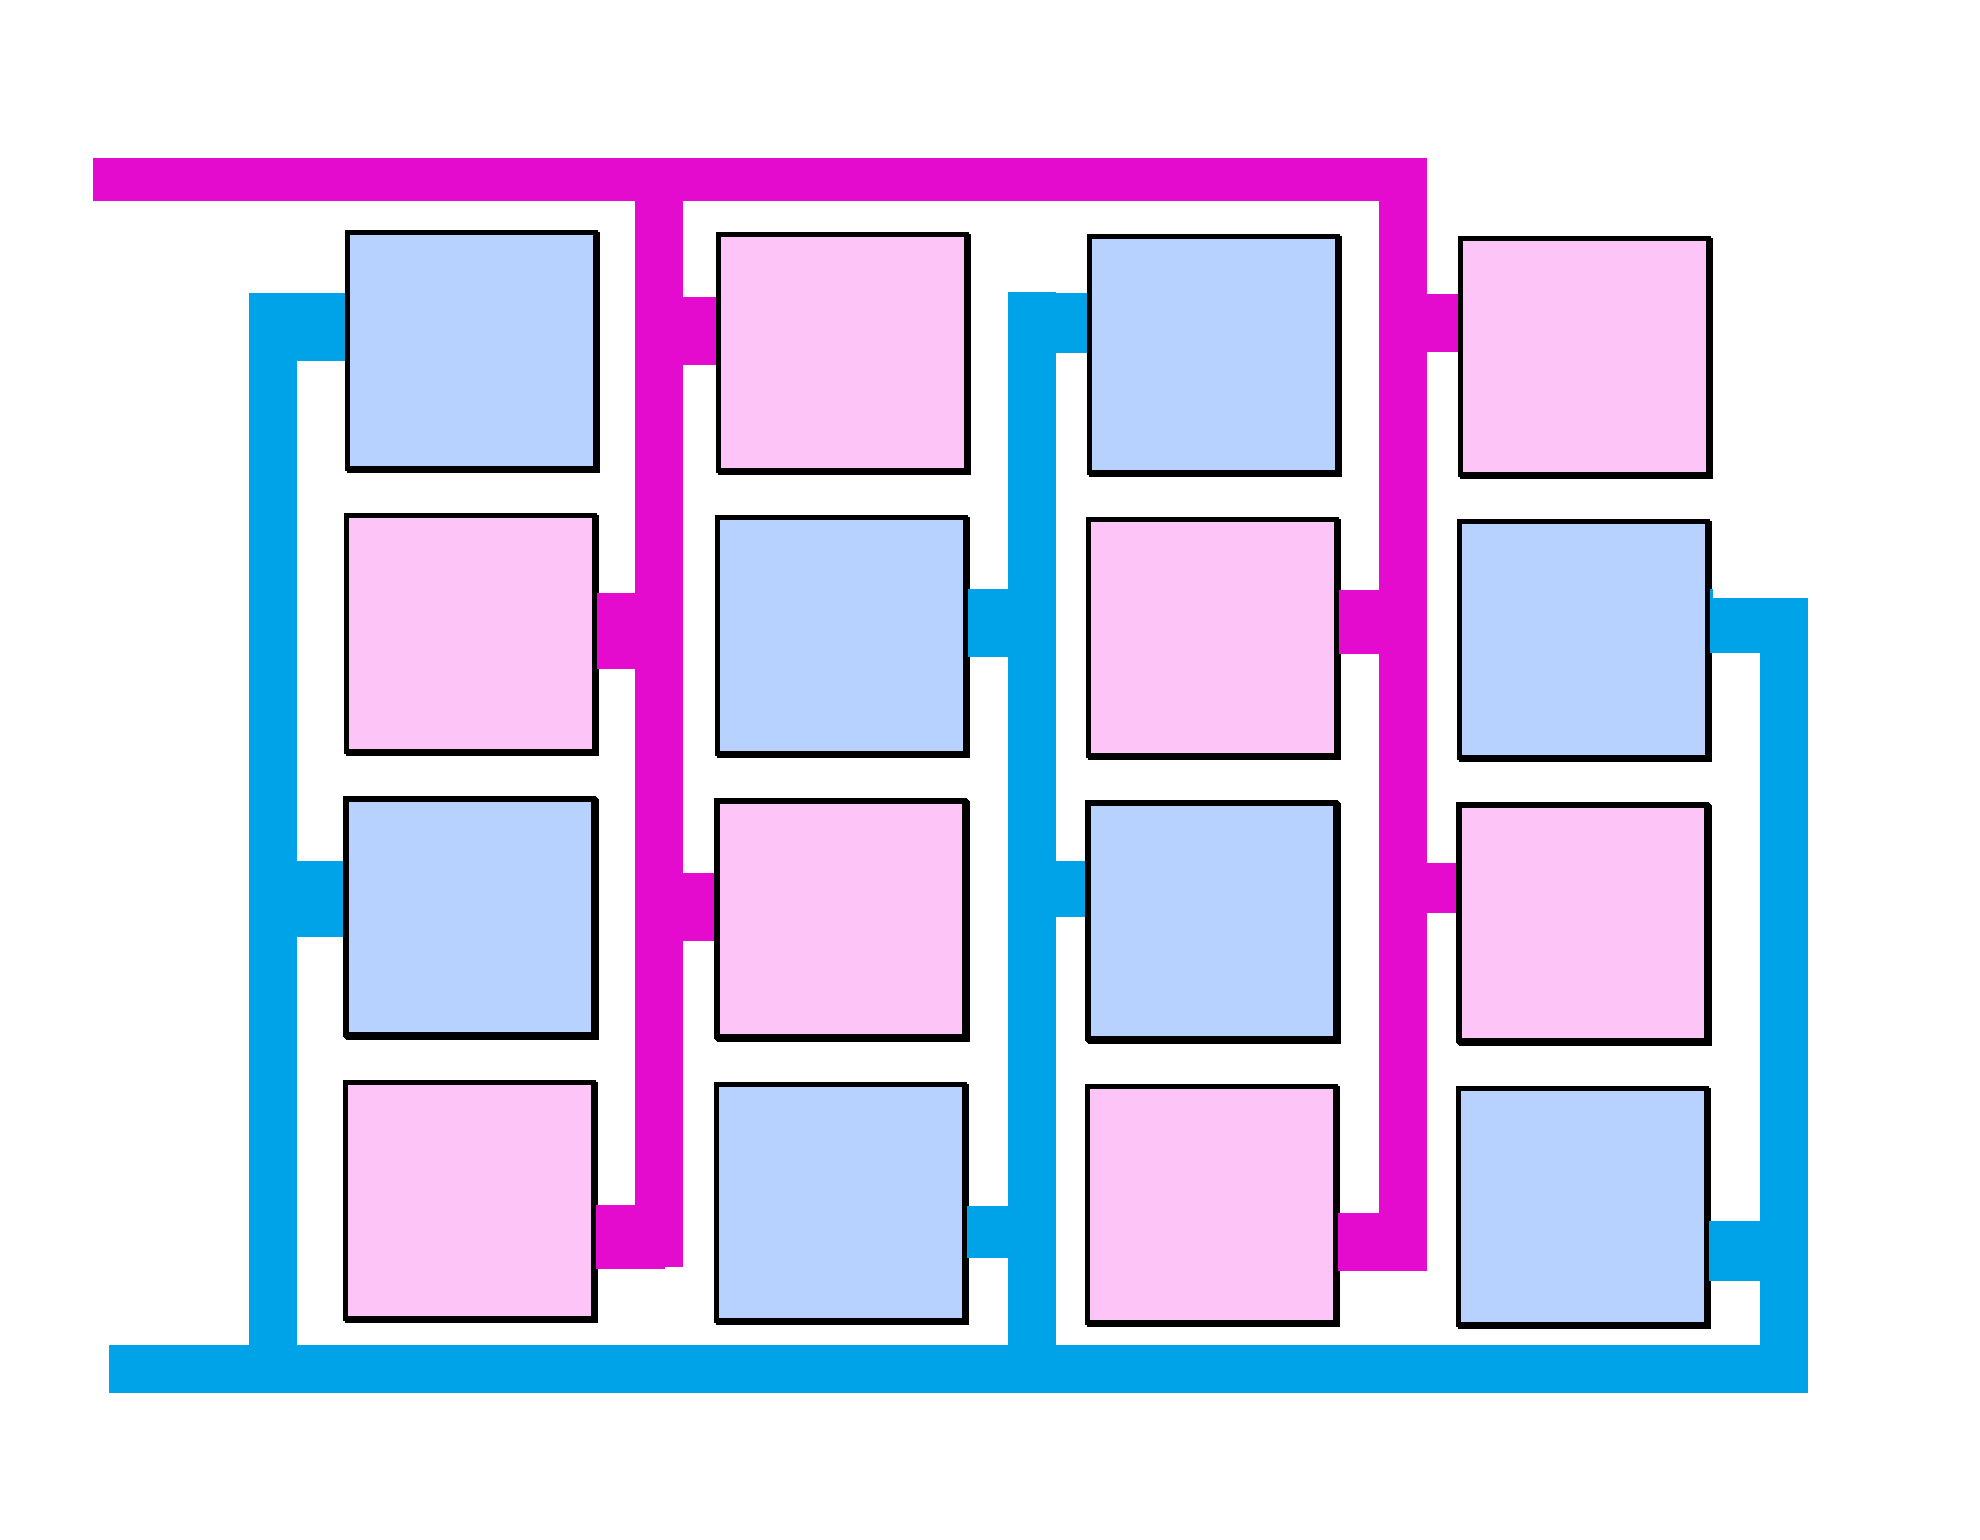
\includegraphics[width=1\textwidth]{Cap1}
		\caption{Bias capacitors layout structure}
		\label{Cap1}
	\end{figure}
\end{columns}
\end{frame}

\begin{frame}
\frametitle{Layout - C\textsubscript{bias}}
\begin{columns}
	\column{0.4\textwidth}
	\begin{itemize}
		\item y = 448.65$\mu$m
		\item x = 472.5$\mu$m
		\item C\textsubscript{bias}=25.9pF
	\end{itemize}
	\column{0.6\textwidth}
	\begin{figure}[H]
		\centering
		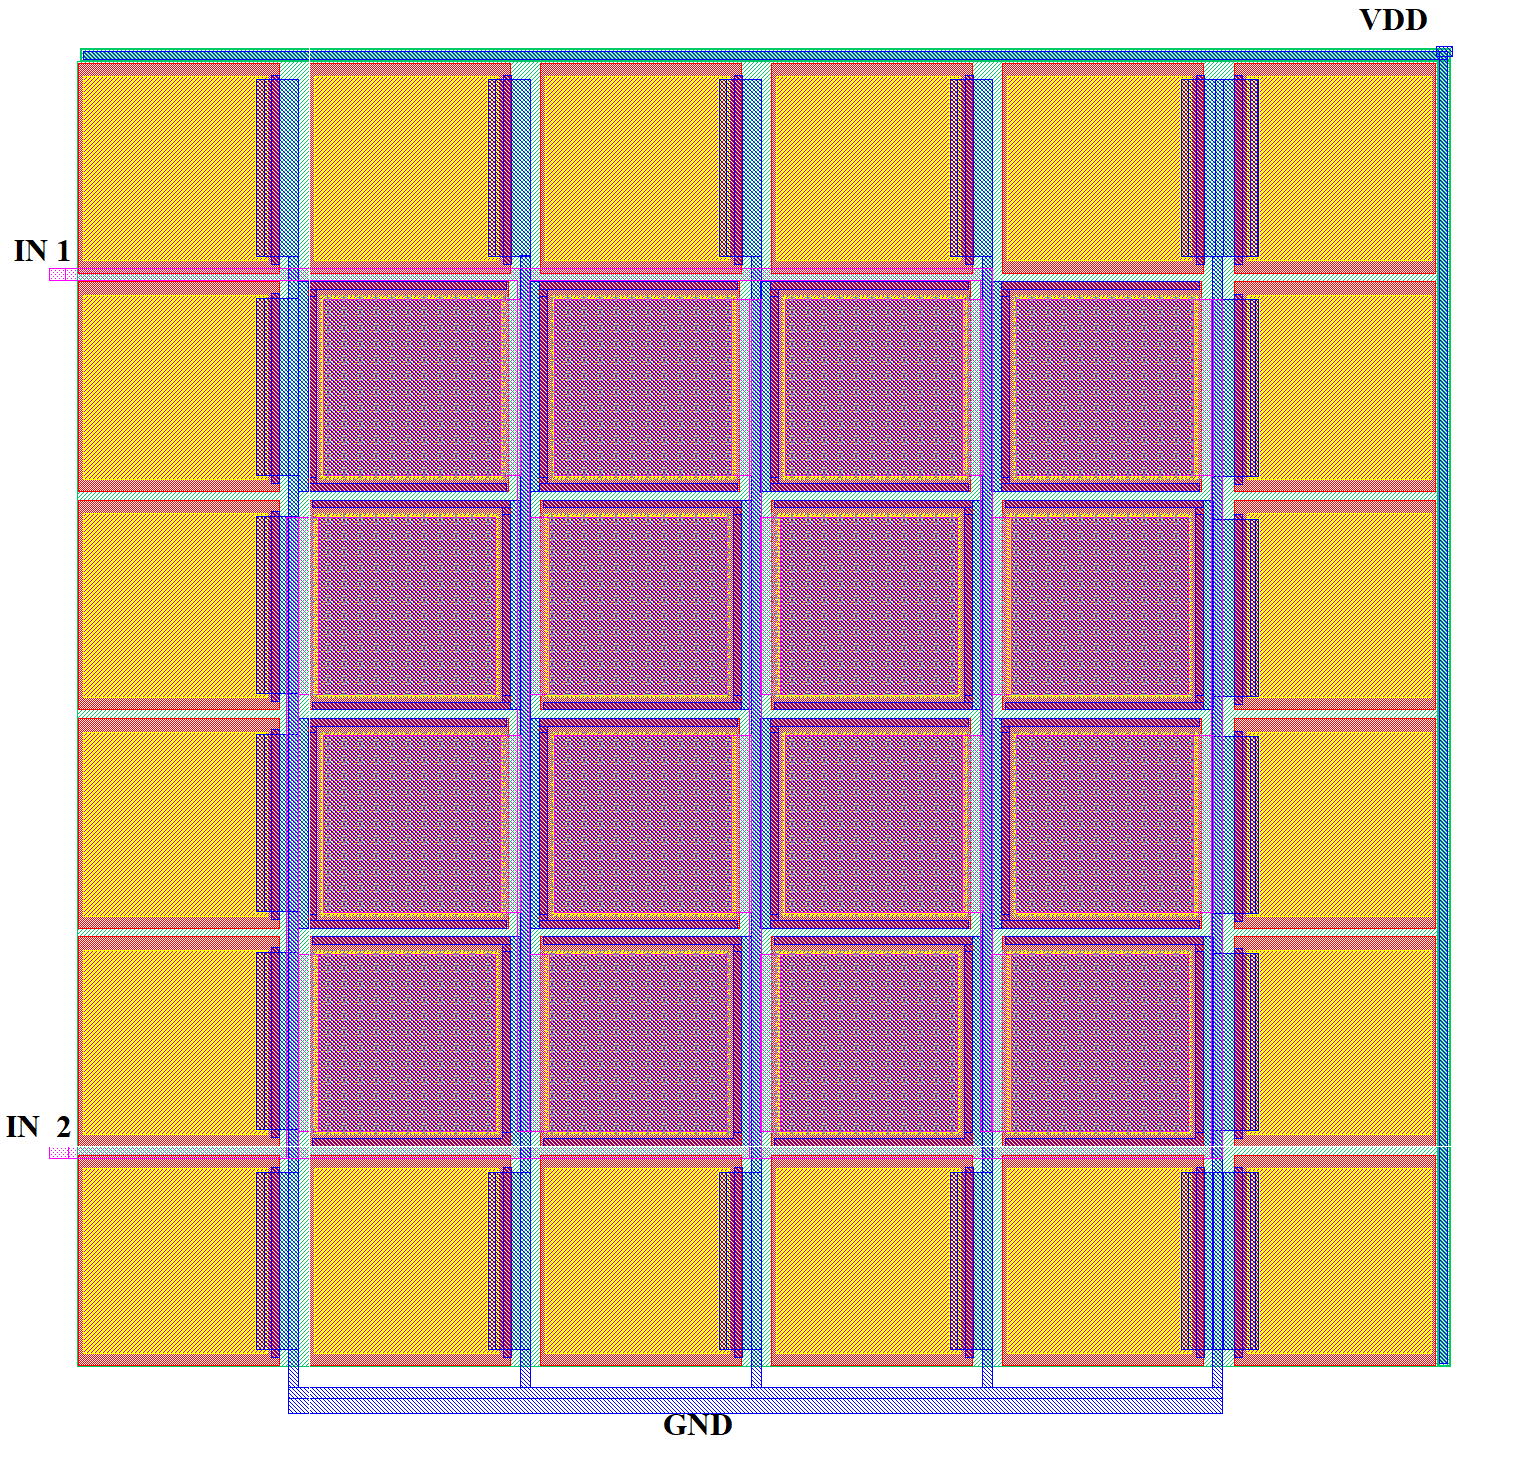
\includegraphics[width=1\textwidth]{L_Cb_full}
		\label{L_Cb_full}
	\end{figure}
\end{columns}
\end{frame}

\begin{frame}
\frametitle{Layout - C\textsubscript{signal}}
\begin{columns}
	\column{0.6\textwidth}
	\begin{itemize}
	\item C\textsubscript{signal} are large capacitances ($\simeq$nF). \item Multilayer structure impossible because of \emph{CMOS design rule 11.6}. \item Good matching required  then common centroid structure is used. \item Series resistance reduced by surrounding metal plates. \item N-well ring connected to V\textsubscript{DD} to reduce fringing field.
	\end{itemize}
	\column{0.4\textwidth}
	\begin{figure}[H]
		\centering
		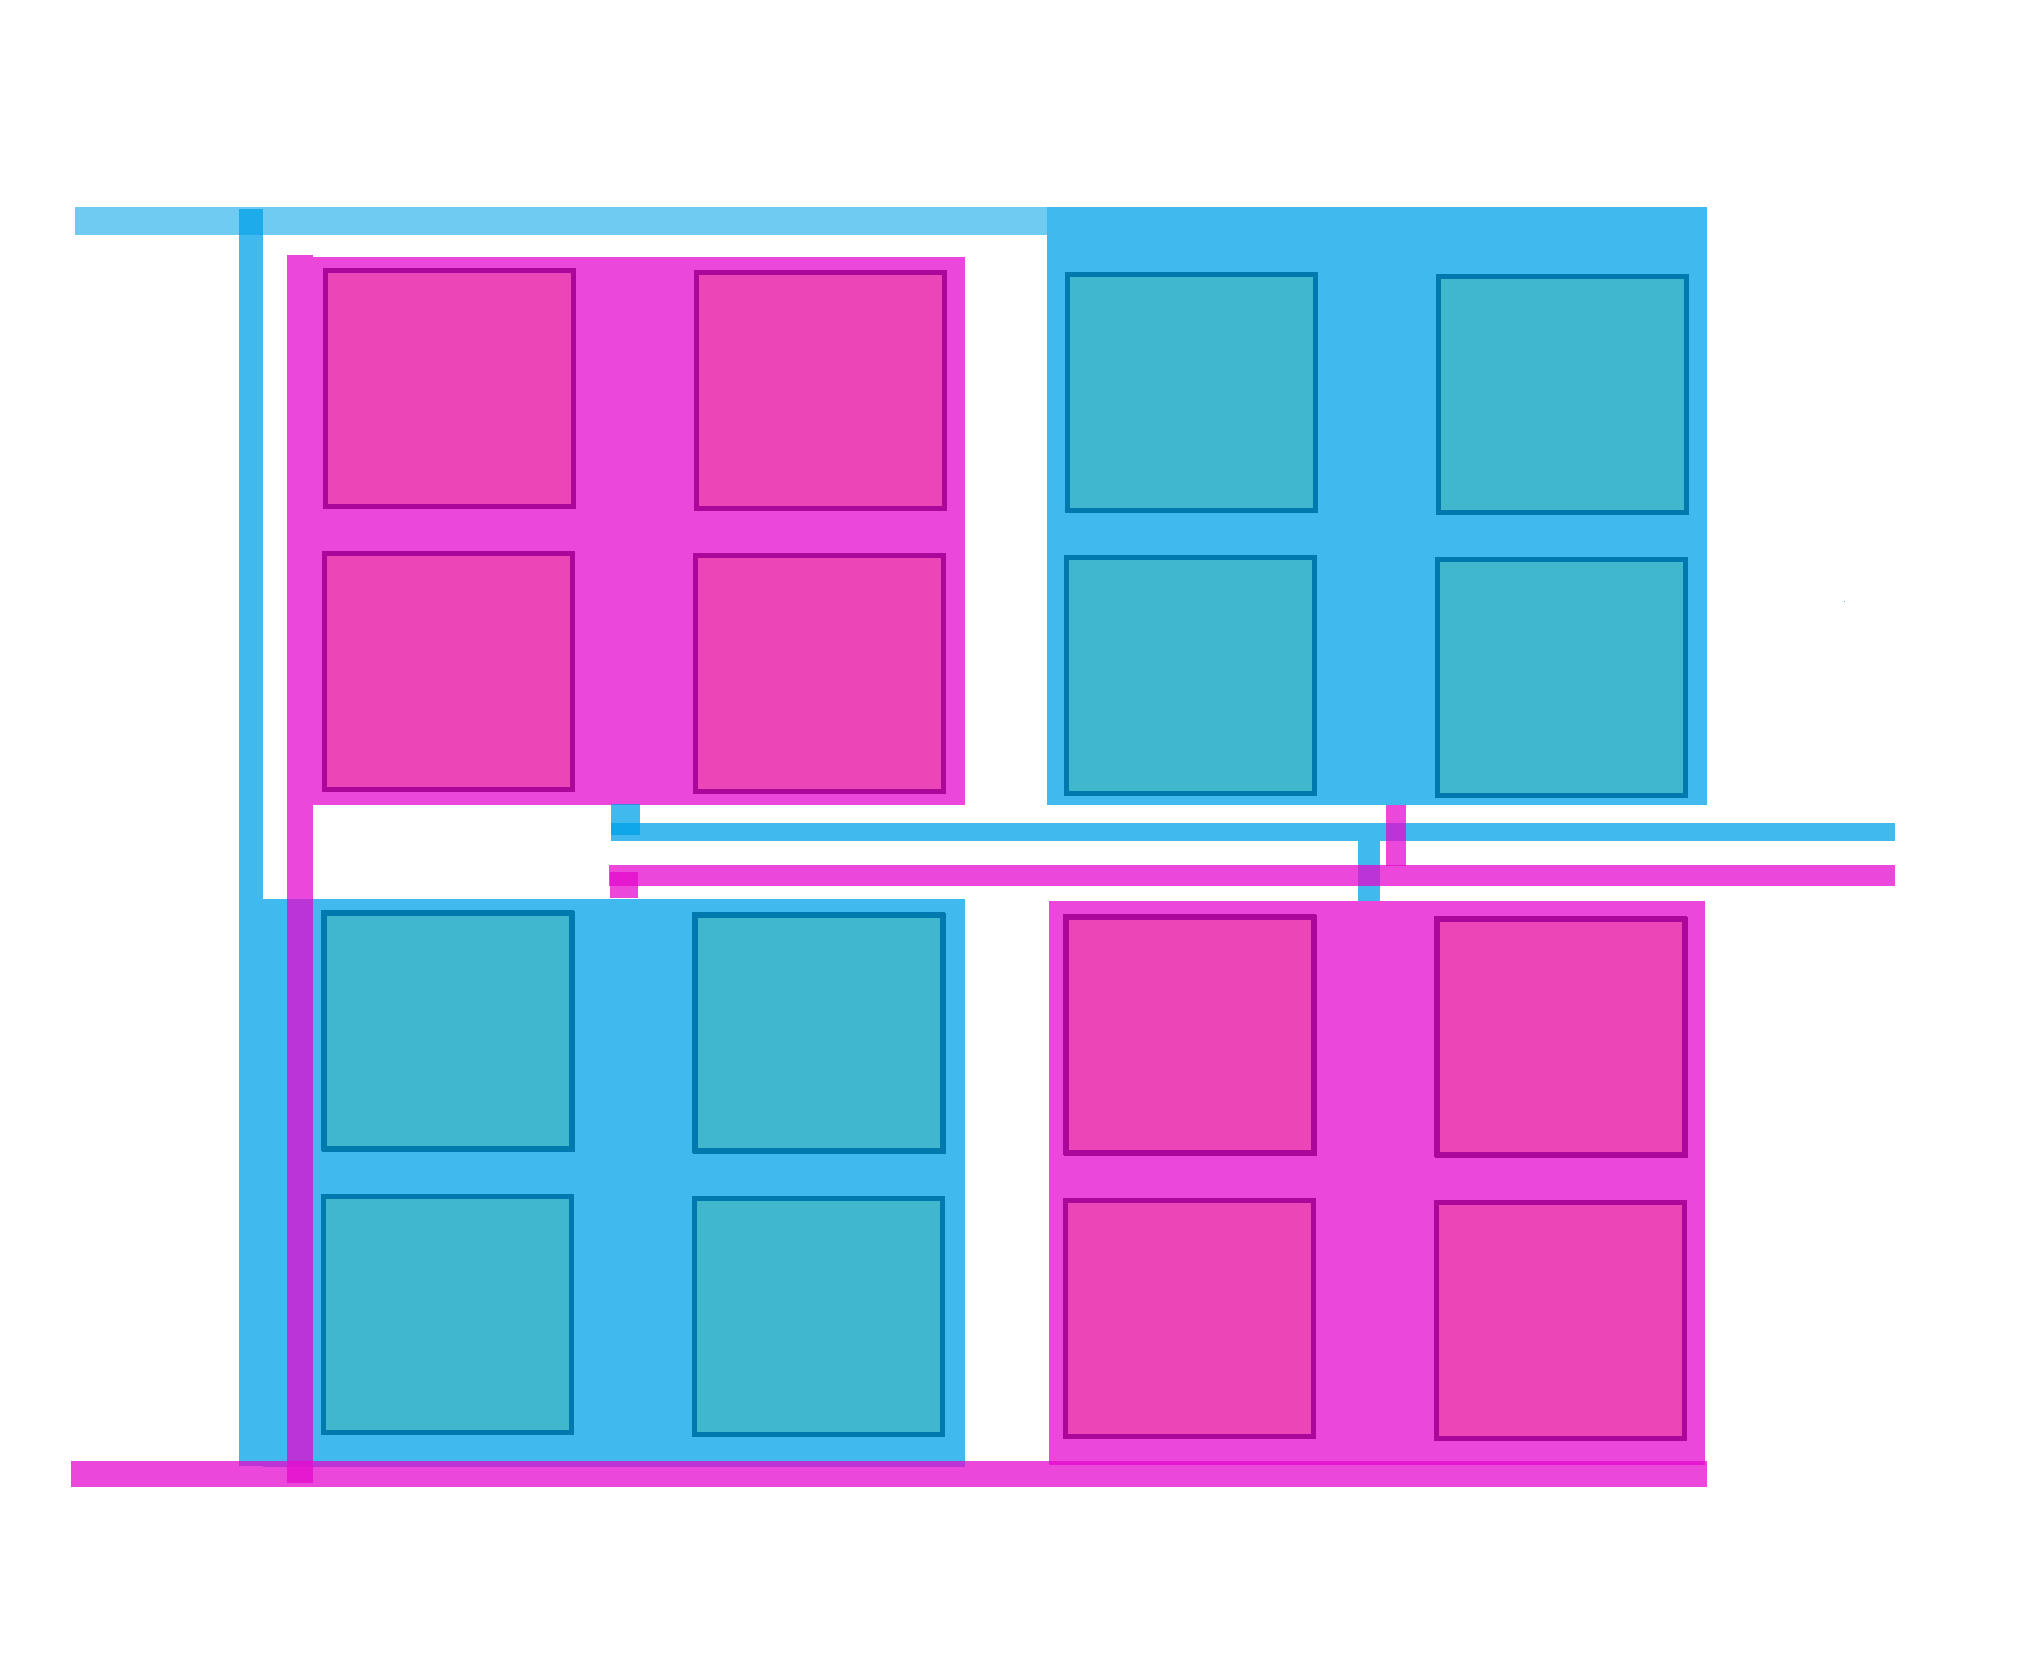
\includegraphics[width=1\textwidth]{Cap2}
		\caption{Common centroid structure of the signal capacitors}
		\label{Cap2}
	\end{figure}
\end{columns}
\end{frame}

\begin{frame}
	\frametitle{Layout - C\textsubscript{signal}}
	\begin{columns}
	\column{0.3\textwidth}
	\begin{itemize}
		\item y = 678.45$\mu$m
		\item x = 480.25$\mu$m
		\item C\textsubscript{bias}=90.1pF
	\end{itemize}
	\column{0.7\textwidth}
	\begin{figure}[H]
		\centering
		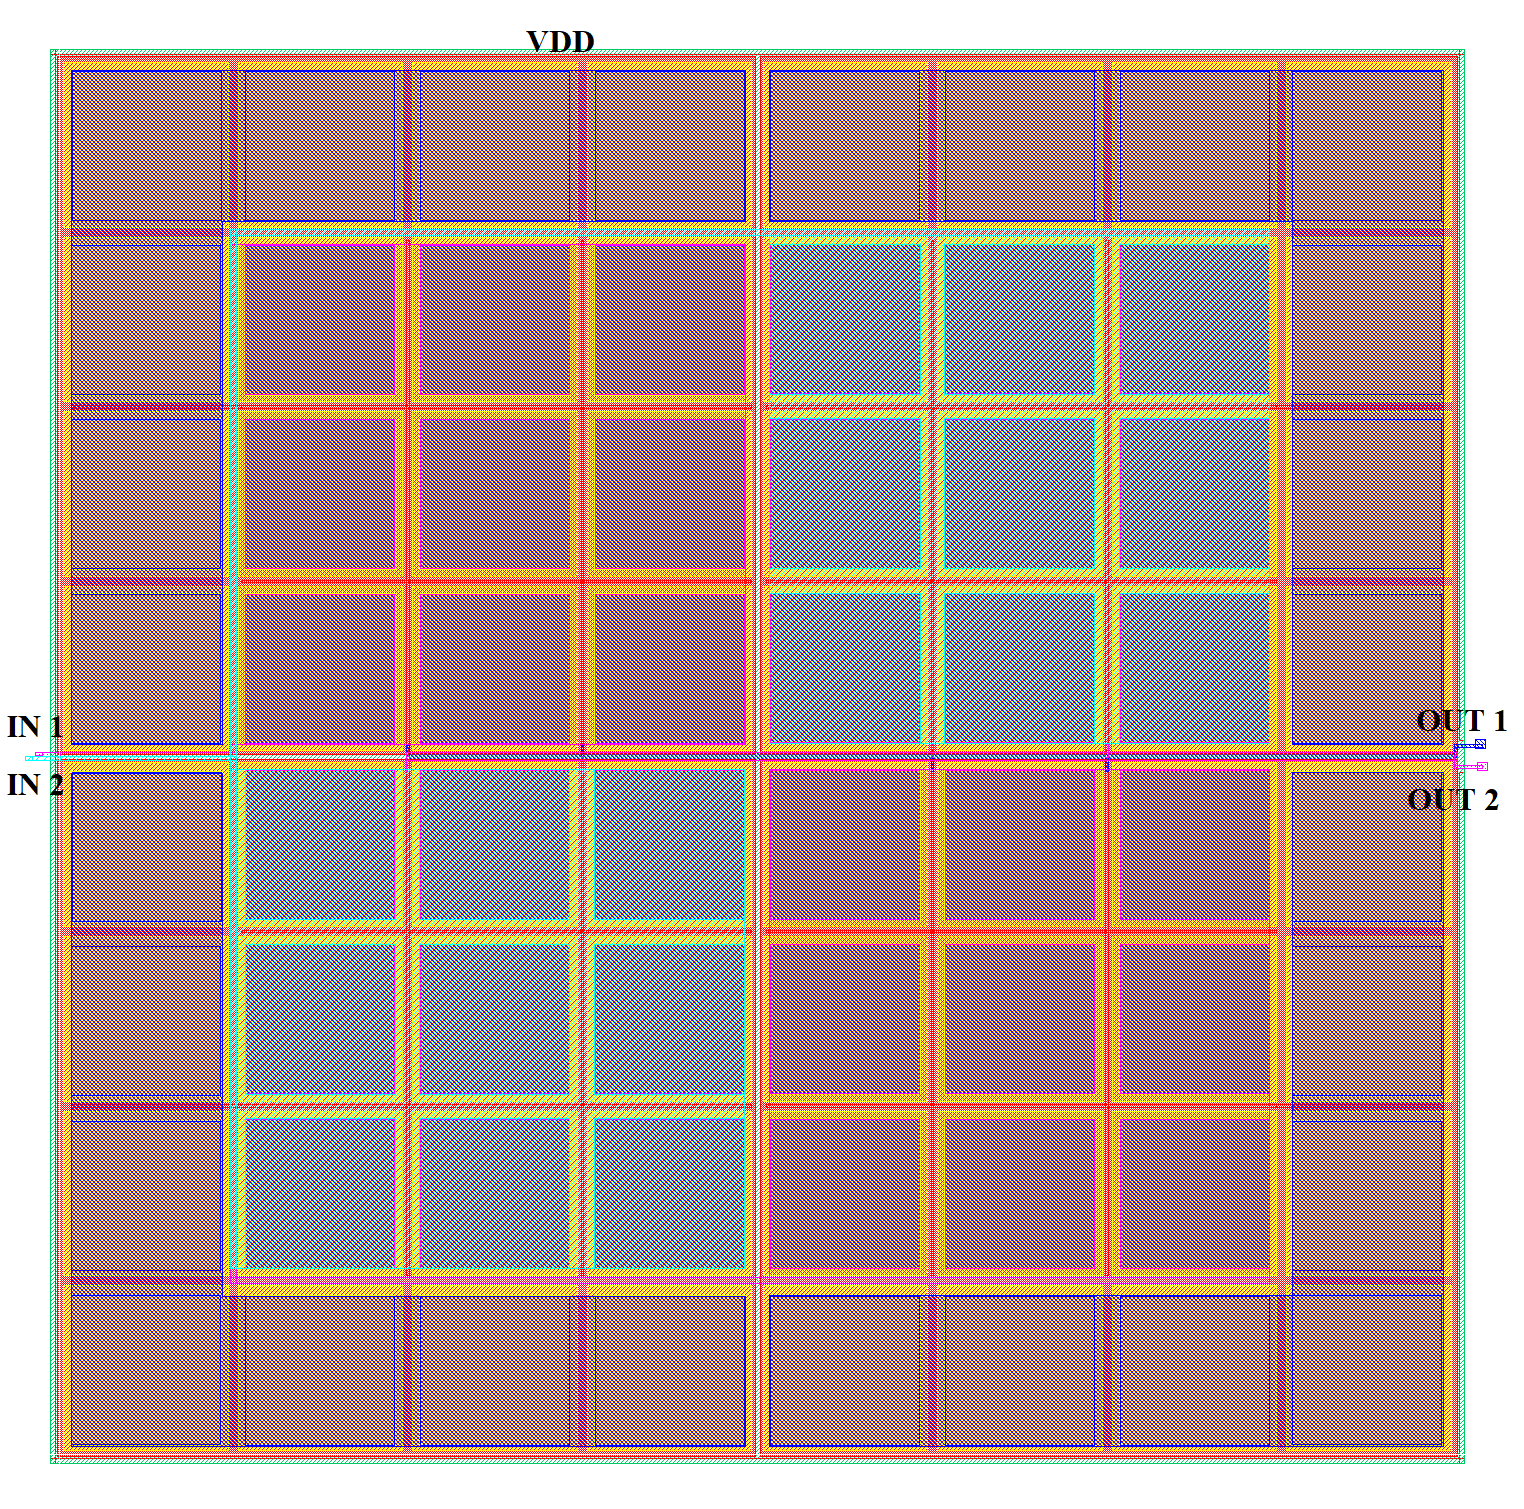
\includegraphics[width=0.7\textwidth]{L_Cs_full}
		\label{L_Cs_full}
	\end{figure}
	\end{columns}
\end{frame}

\begin{frame}
\frametitle{Layout - R\textsubscript{1,3}}
\begin{columns}
	\column{0.5\textwidth}
	\begin{itemize}
	\item R\textsubscript{1,3} are large, then n-well technology necessary with common centroid structure to improve gradients (precision not necessary though). 
	\item Since nearby mixing stage guard ring needed to avoid substrate currents.
	\end{itemize}
	\column{0.5\textwidth}
	\begin{figure}[H]
		\centering
		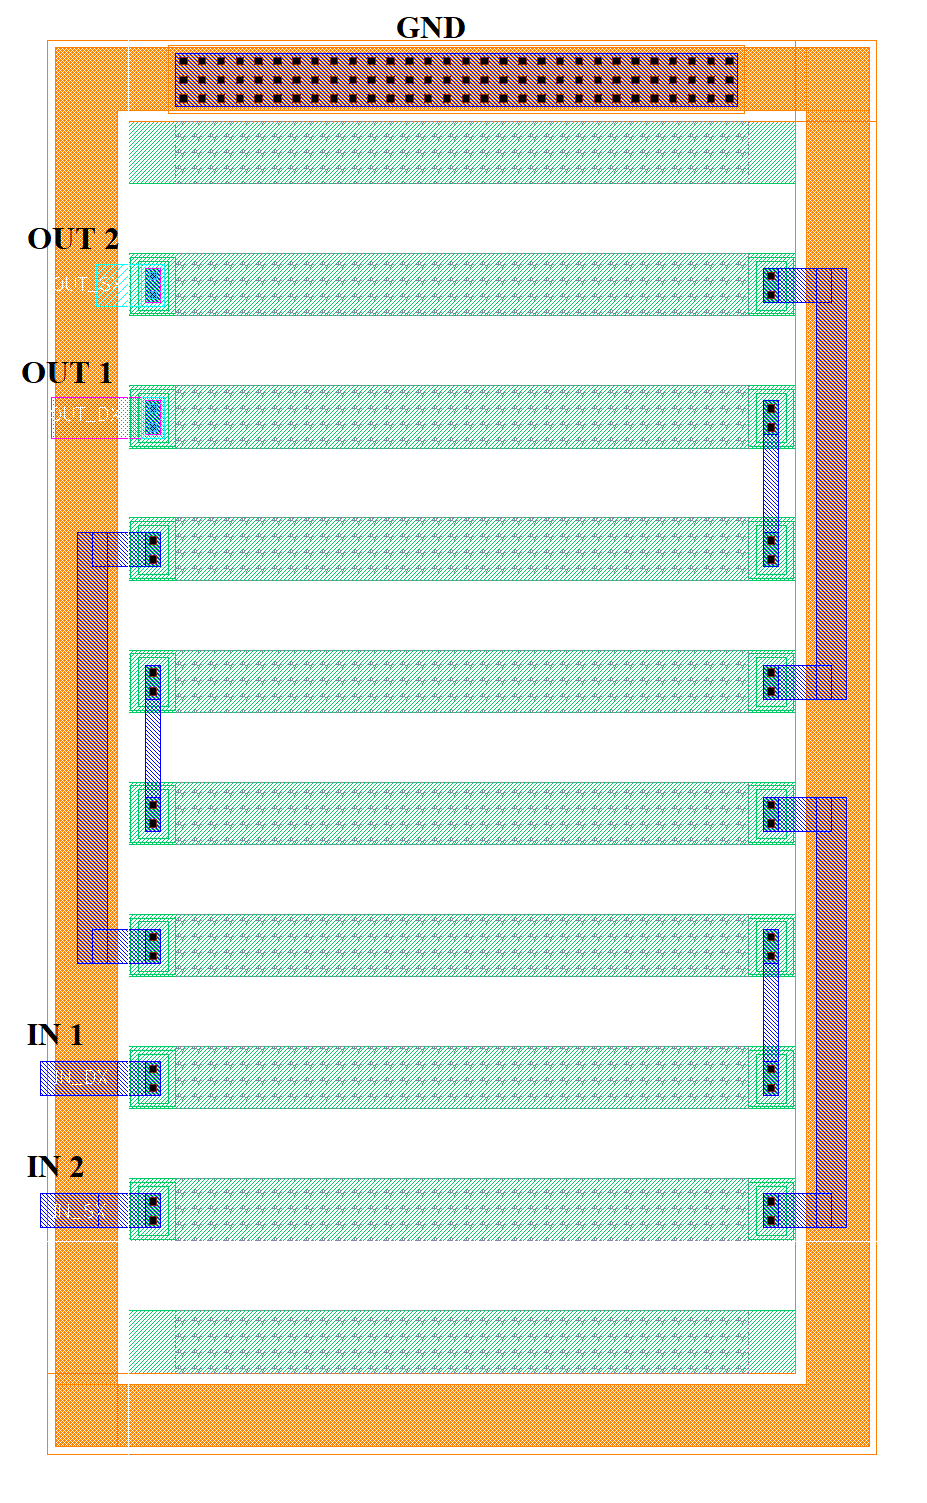
\includegraphics[scale=0.15]{L_R1R3}
		\label{L_R1R3}
	\end{figure}
\end{columns}
\end{frame}

\begin{frame}
\frametitle{Layout - R\textsubscript{2},R\textsubscript{4},R\textsubscript{L},R\textsubscript{S}}
\begin{columns}
	\column{0.5\textwidth}
	\begin{itemize}	
	\item R\textsubscript{2},R\textsubscript{4},R\textsubscript{L} and R\textsubscript{S} are smaller than R\textsubscript{1,3} therefore poly1 resistors can be used, improving also precision. 
	\item Common centroid structure with dummy elements.
	\end{itemize}
	\column{0.5\textwidth}
	\begin{figure}[H]
		\centering
		
		\subfloat[$R_2$\label{subfig-1:L_R2}]
		{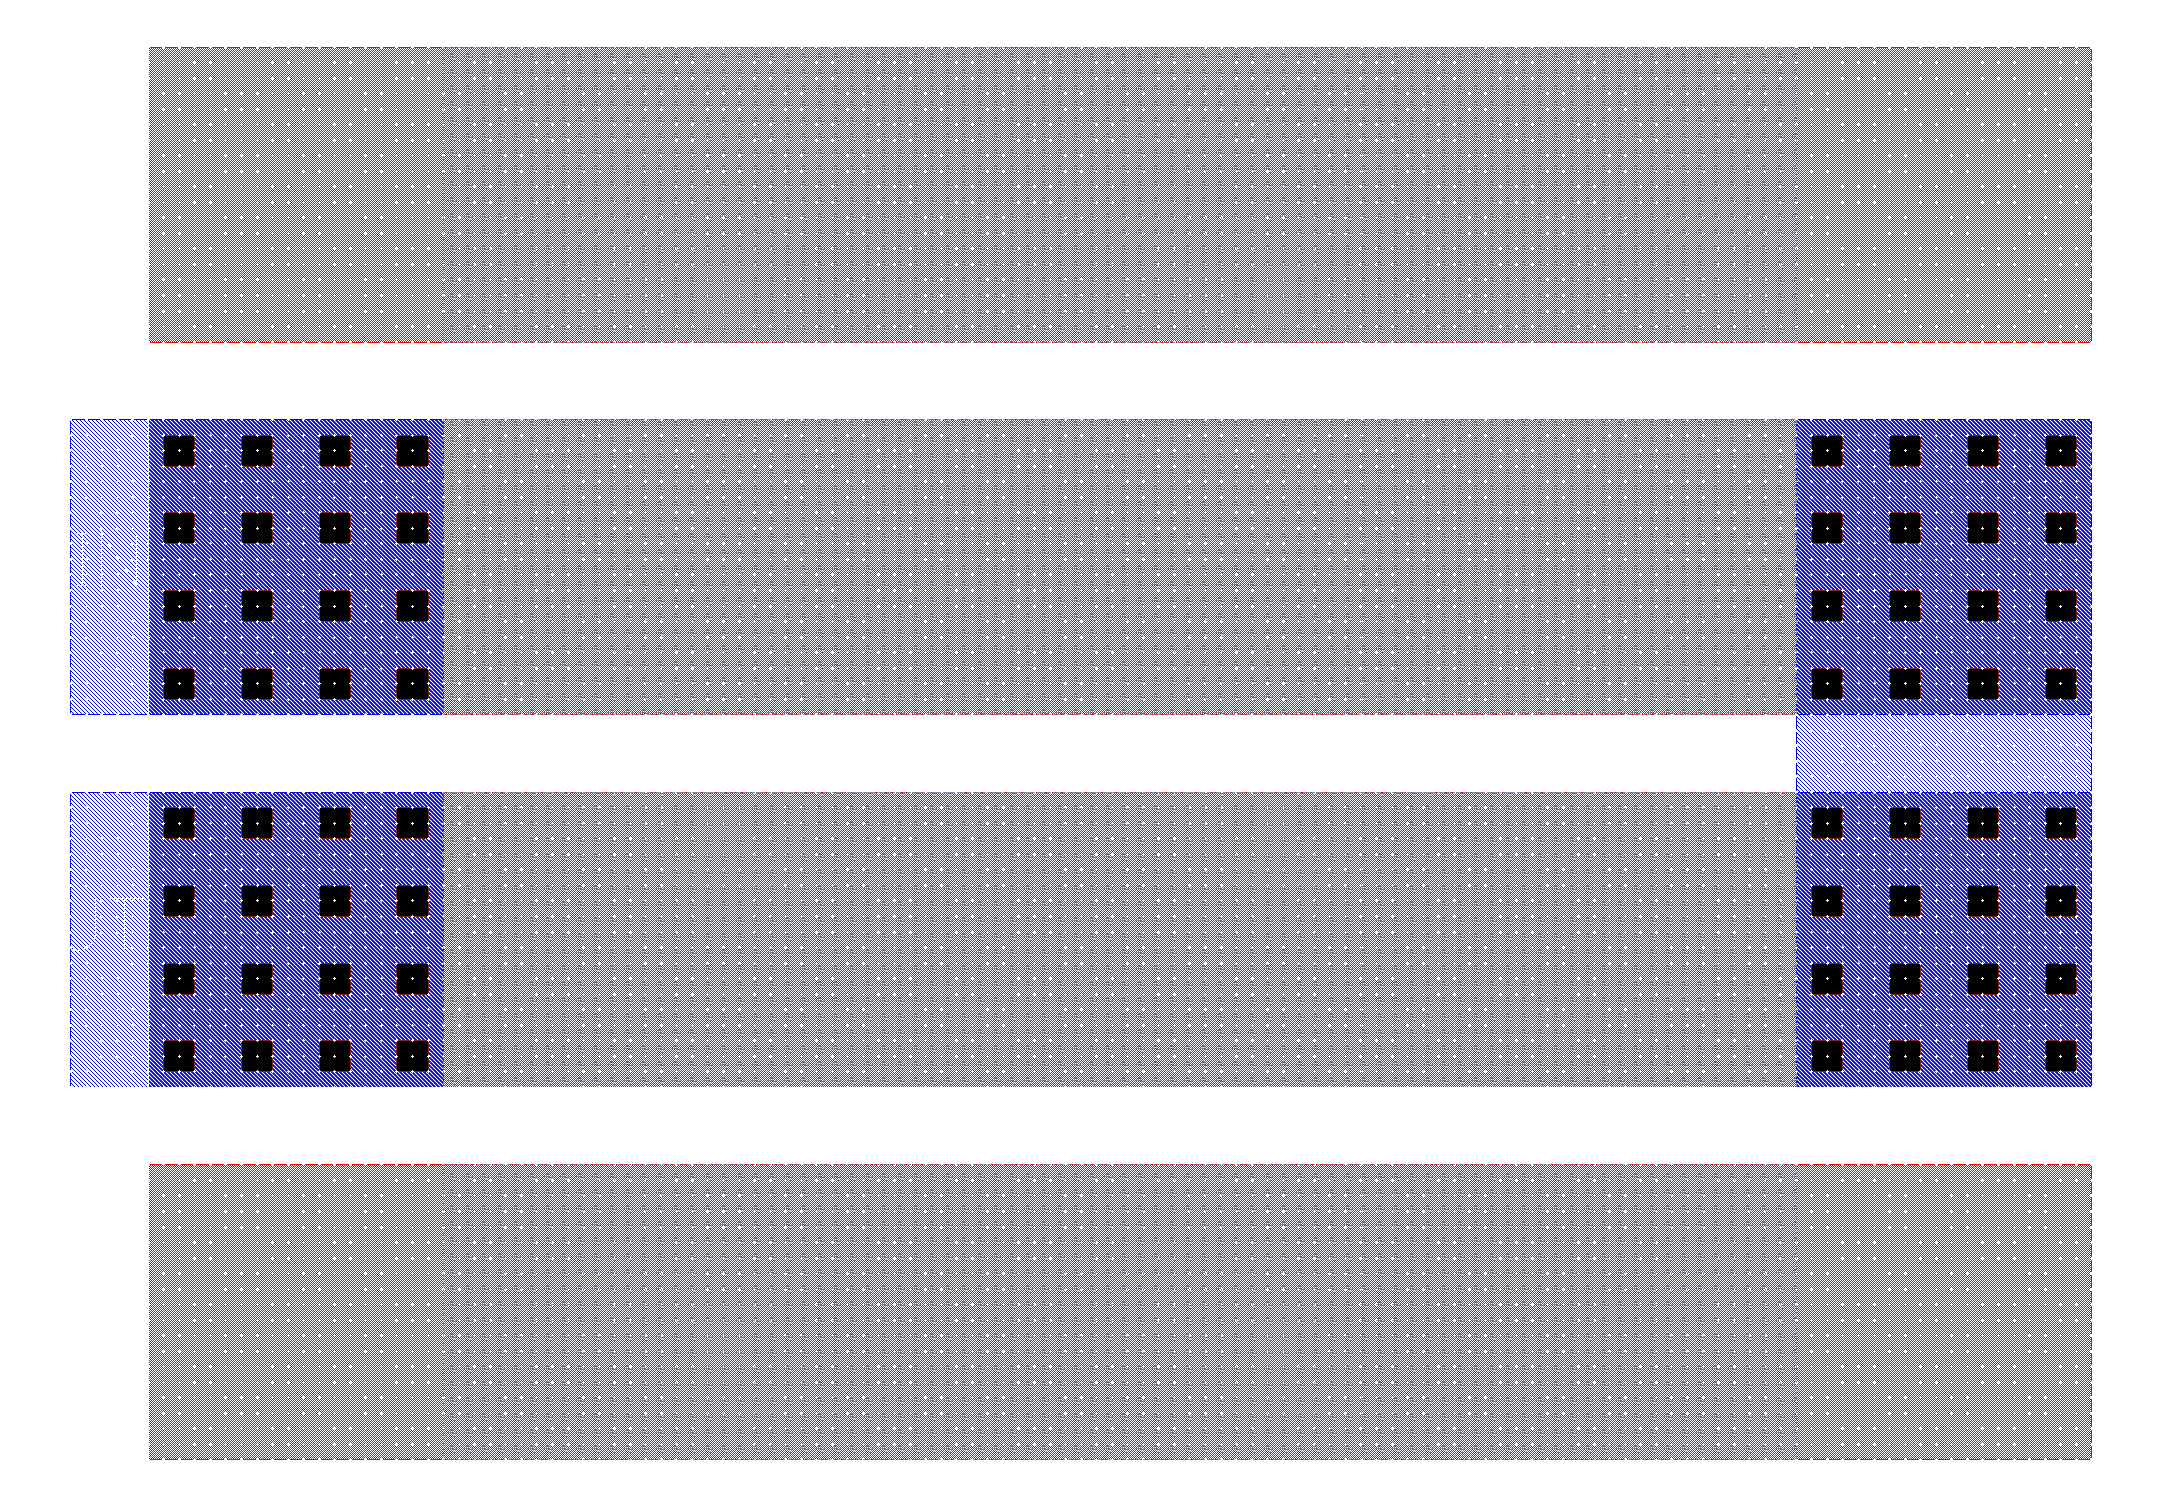
\includegraphics[width=0.4\textwidth]{L_R2}}
		\subfloat[$R_4$\label{subfig-1:L_R4}]
		{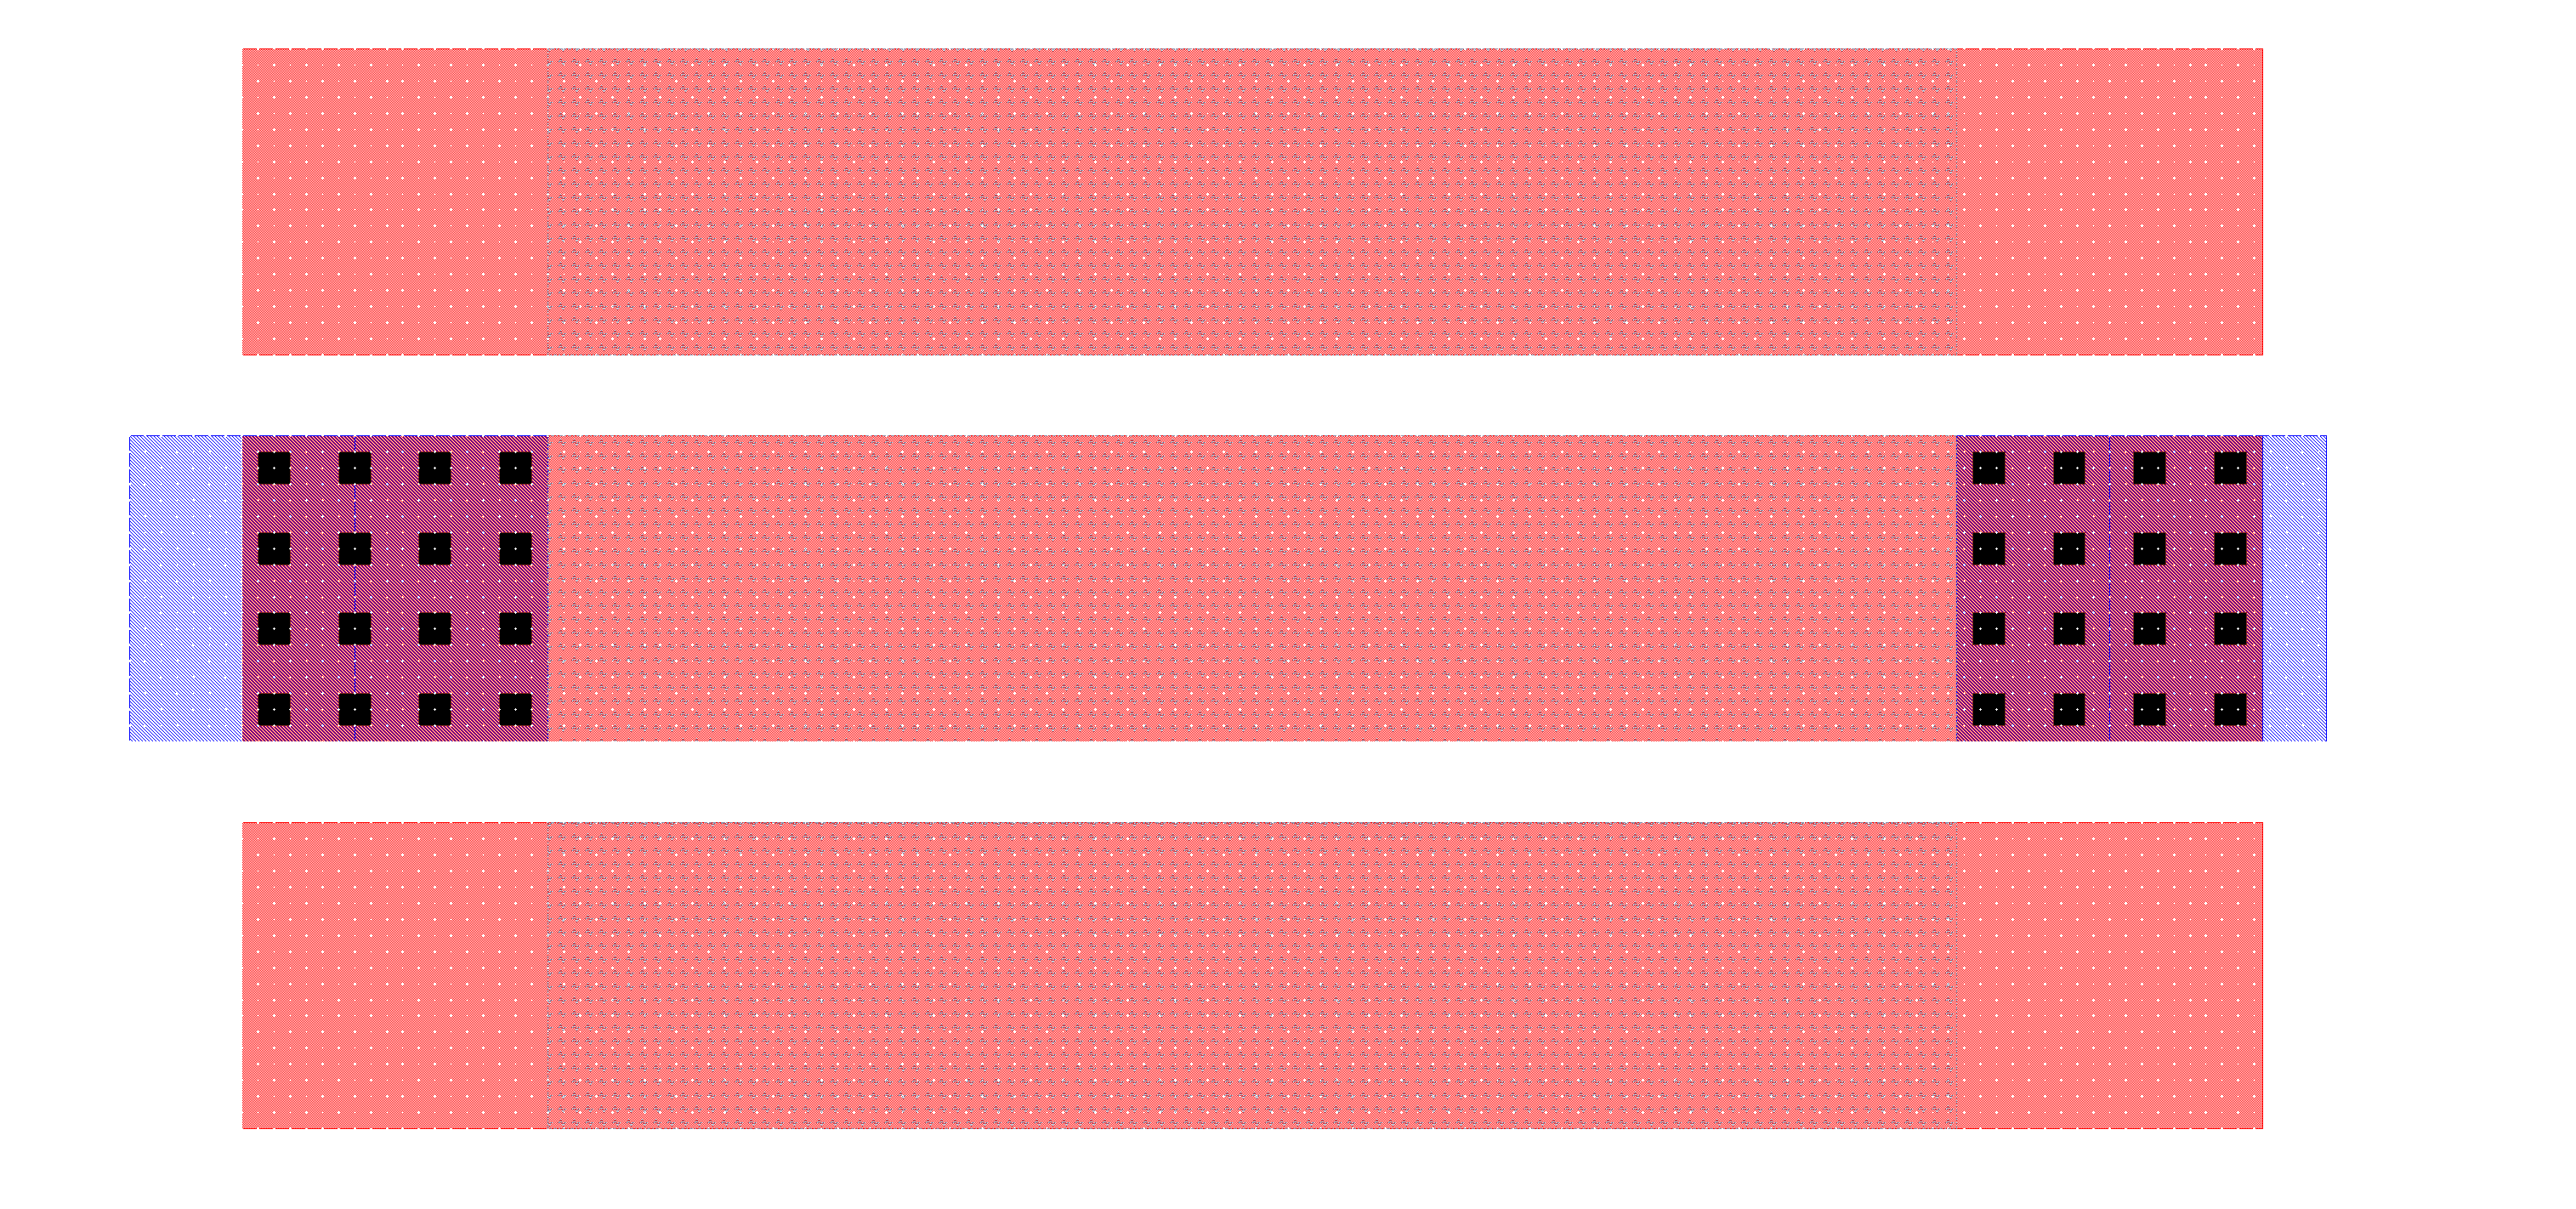
\includegraphics[width=0.5\textwidth]{L_R4}}
		\vfill
		\subfloat[$R_L$\label{subfig-1:L_RL}]
		{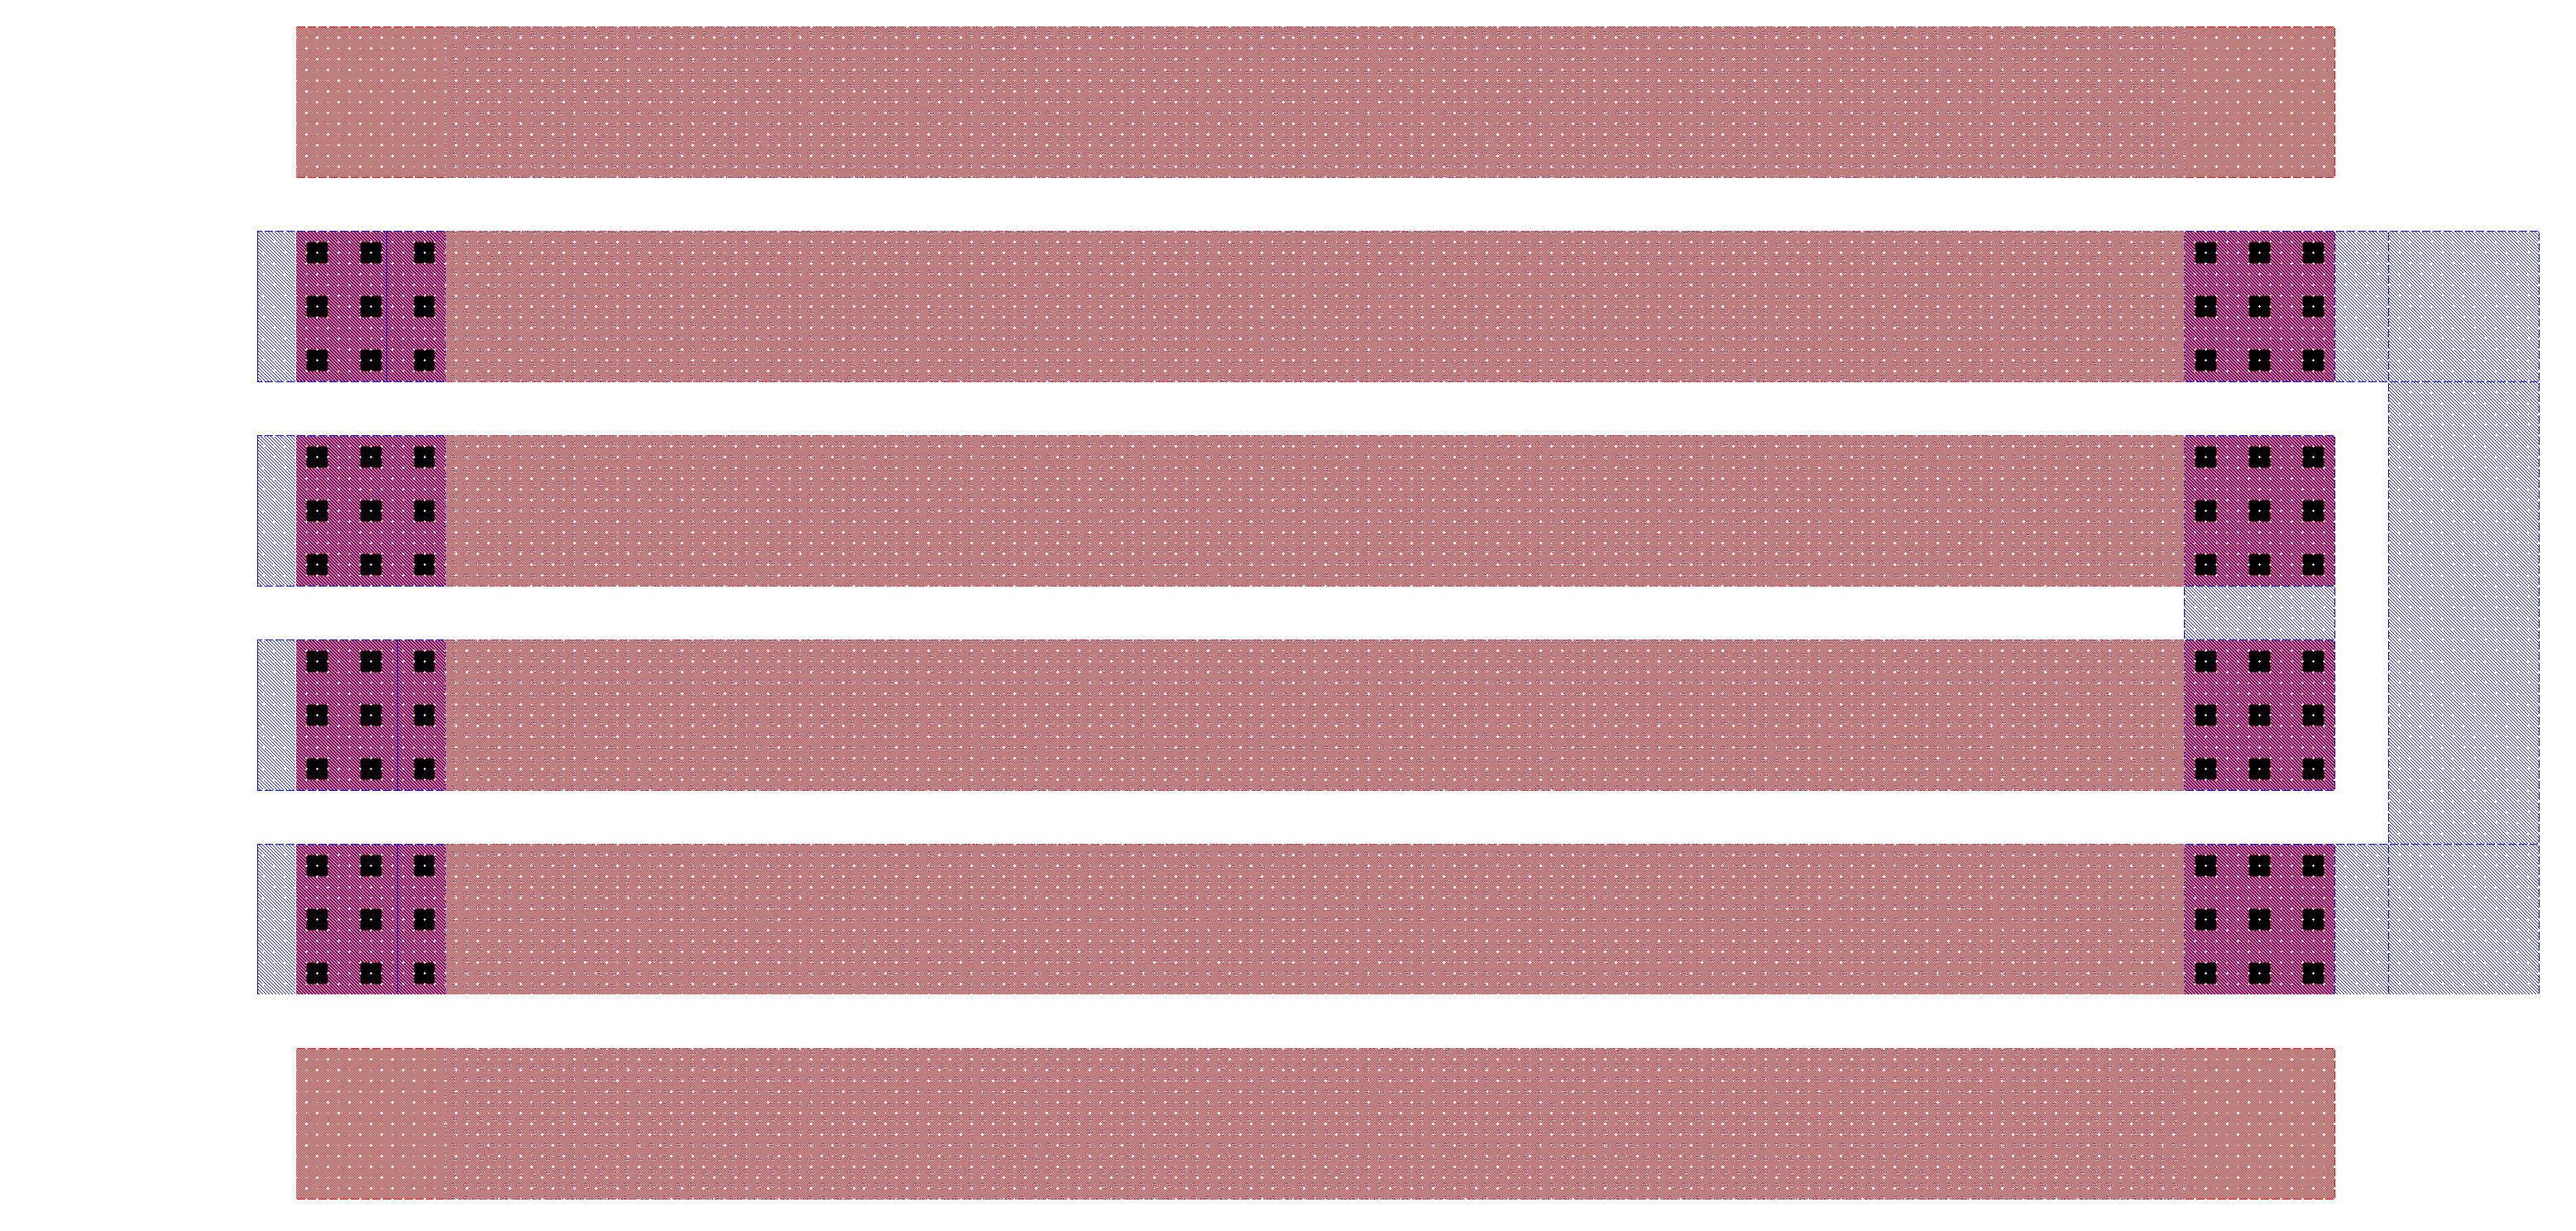
\includegraphics[width=0.55\textwidth]{L_RL}}
		\hfil
		\subfloat[$R_S$\label{subfig-1:L_RS}]
		{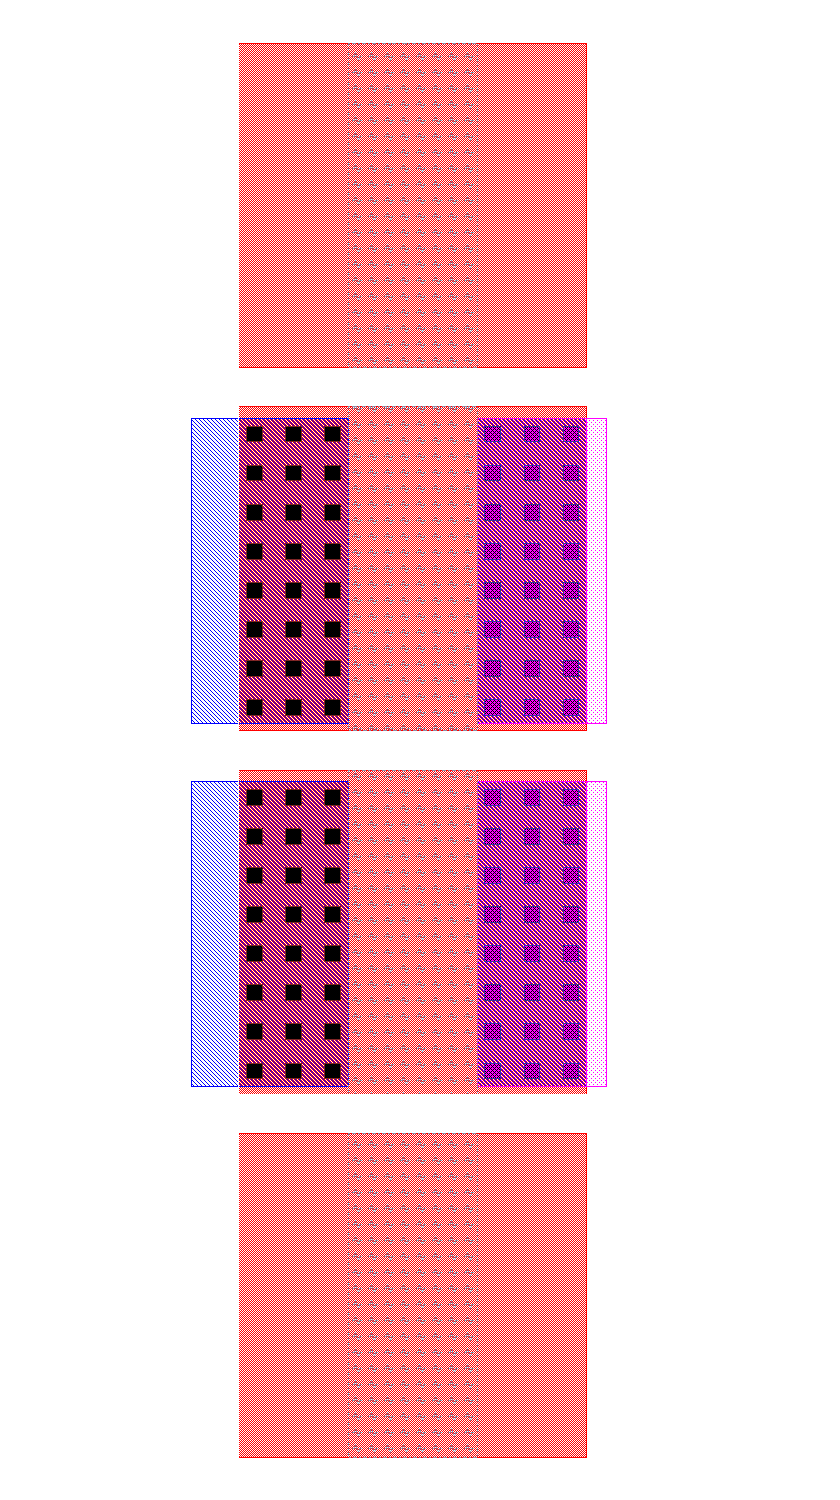
\includegraphics[width=0.2\textwidth]{L_RS}}
		\caption{Poly resistors layout}
	\end{figure}
\end{columns}
\end{frame}

\begin{frame}
	\frametitle{Layout - Resistors parameters}
	\begin{table} [h]
		\label{tab:specs}
		\caption{Resistors parameters}
		\centering	
		\begin{tabular}{lccccc} 
			\toprule 
			Parameter & R\textsubscript{1,3}& R\textsubscript{2} & R\textsubscript{4}&R\textsubscript{L}&R\textsubscript{S} \\ 
			\midrule
			y [$\mu m$] &112.05&27.45&20.1&32.4&54\\
			x [$\mu m$] &66.3&37.35&37.65&63&13.35\\
			h [$\mu m$] &4.95&5.7&5.7&4.2&12.45\\
			w [$\mu m$] &46.5&26.1&26.25&48.6&4.95\\
			m			&4&2&1&1&1\\
			R$^*$ [$\Omega$] & 7545&114.5&115.1&289.3&9.94\\
			R\textsubscript{tot} [$\Omega$]&30180&229&115.1&289.3&9.94\\
			\bottomrule 
		\end{tabular}	
	\end{table}

\end{frame}

\begin{frame}
	\frametitle{Layout - Full circuit}
	Merging:
	\begin{itemize}
		\item Components placed to shorten interconnections, emphasize symmetries and matching to make paths equal for high frequency signals;
		\item Body contacts placed where possible, then connected to ground, to capture free charges in the substrate (less noise).
		\item Occupied area: $A\simeq0.7mm \cdot 1.8mm = 1.26 mm^2$;
		\item Large amount of area occupied by capacitors.
	\end{itemize}
\end{frame}

\begin{frame}
	\frametitle{Layout - Full circuit}
	\begin{figure}[H]
		\centering
		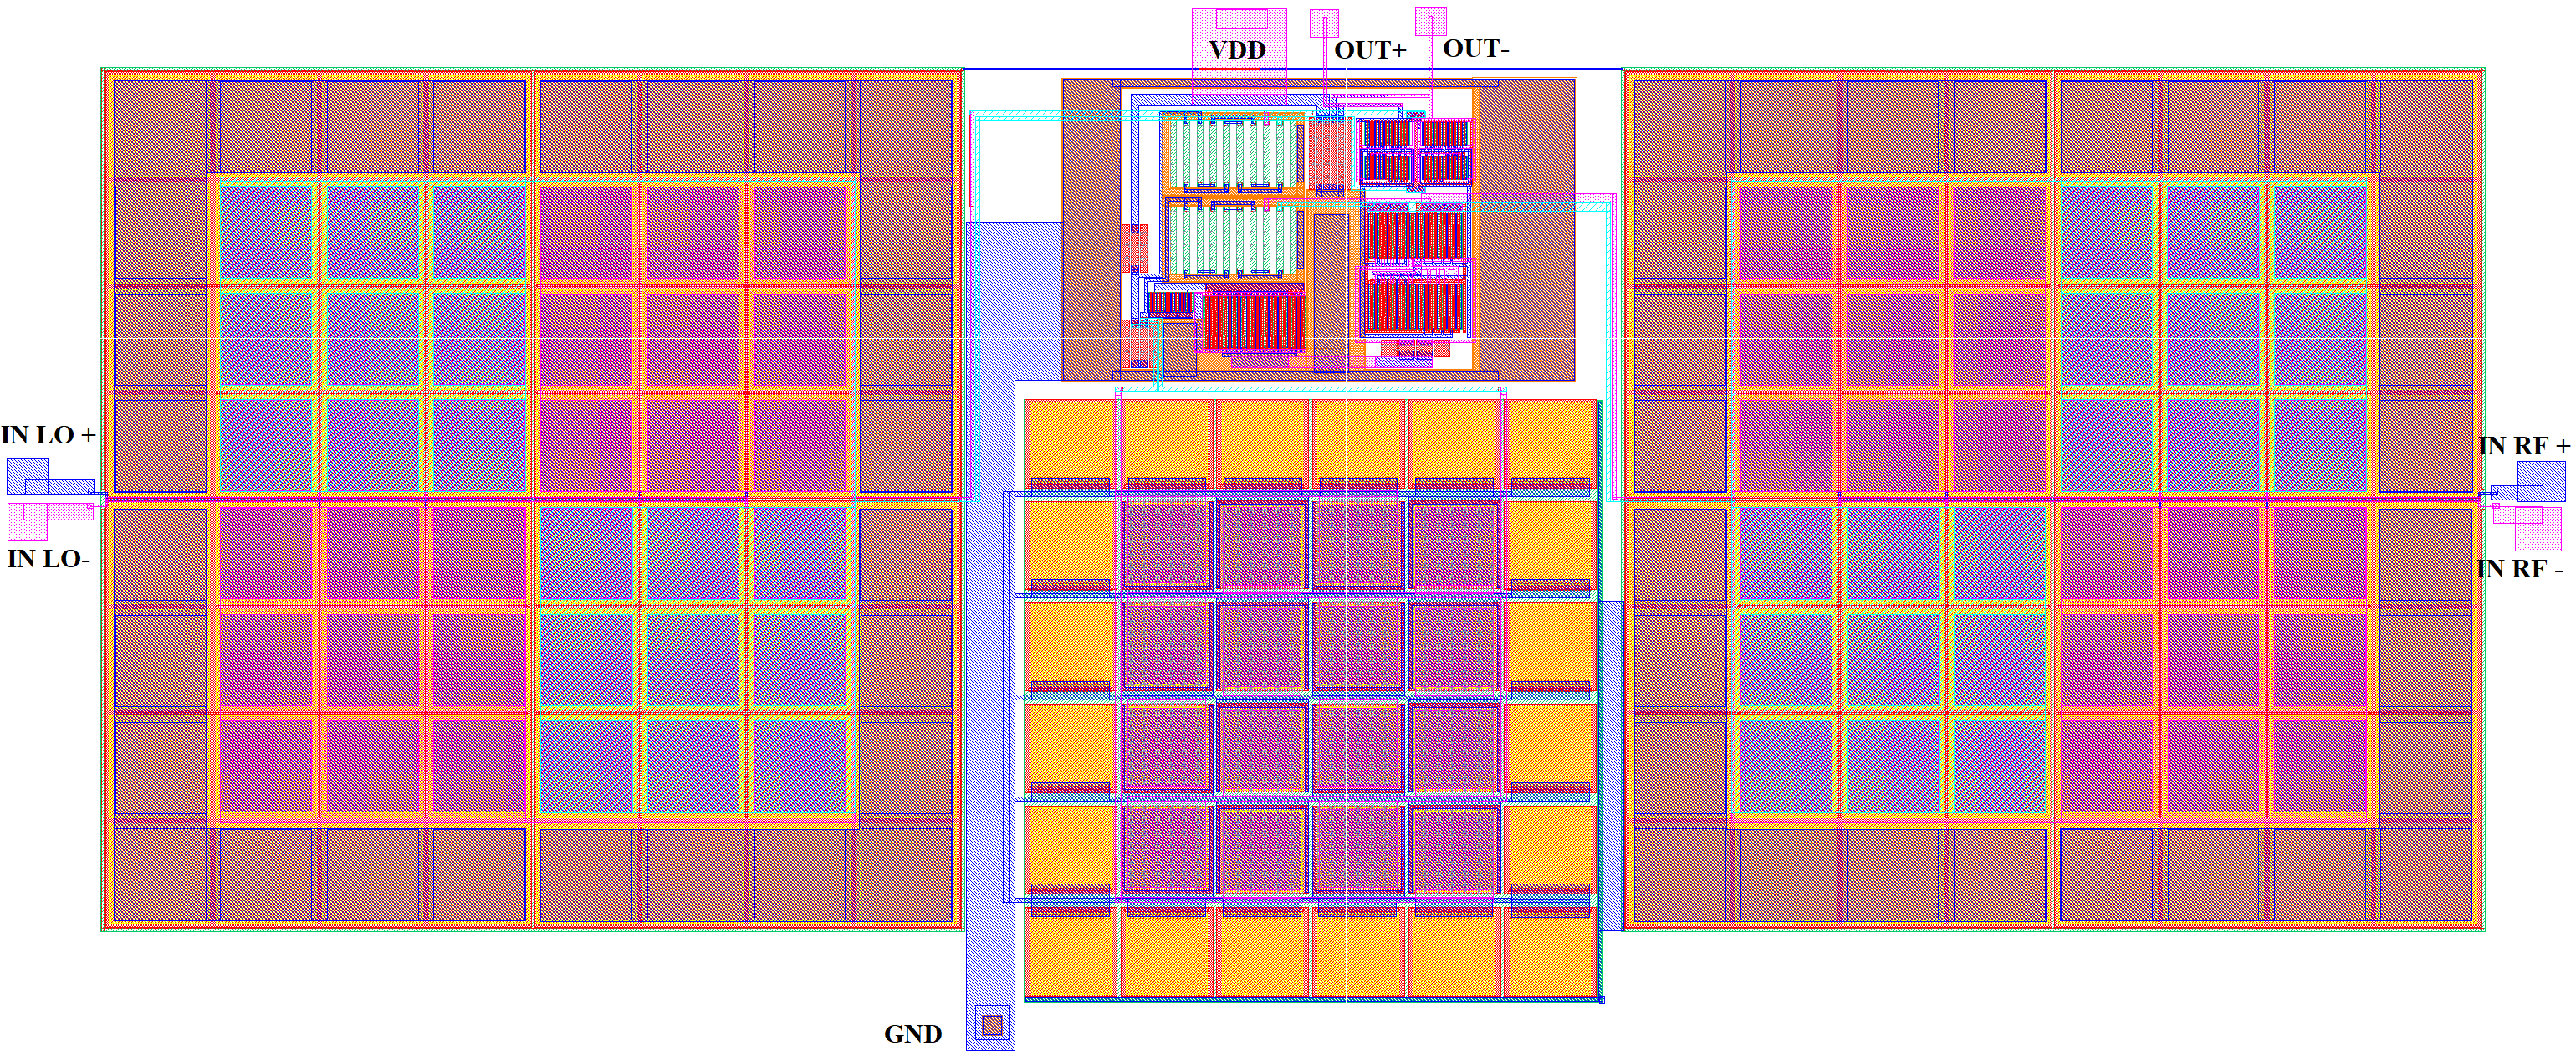
\includegraphics[width=1\textwidth]{L_complete_full}
		\label{L_complete_full}
	\end{figure}
\end{frame}

\begin{frame}
	\frametitle{Layout - Full circuit without capacitors}
	\begin{figure}[H]
		\centering
		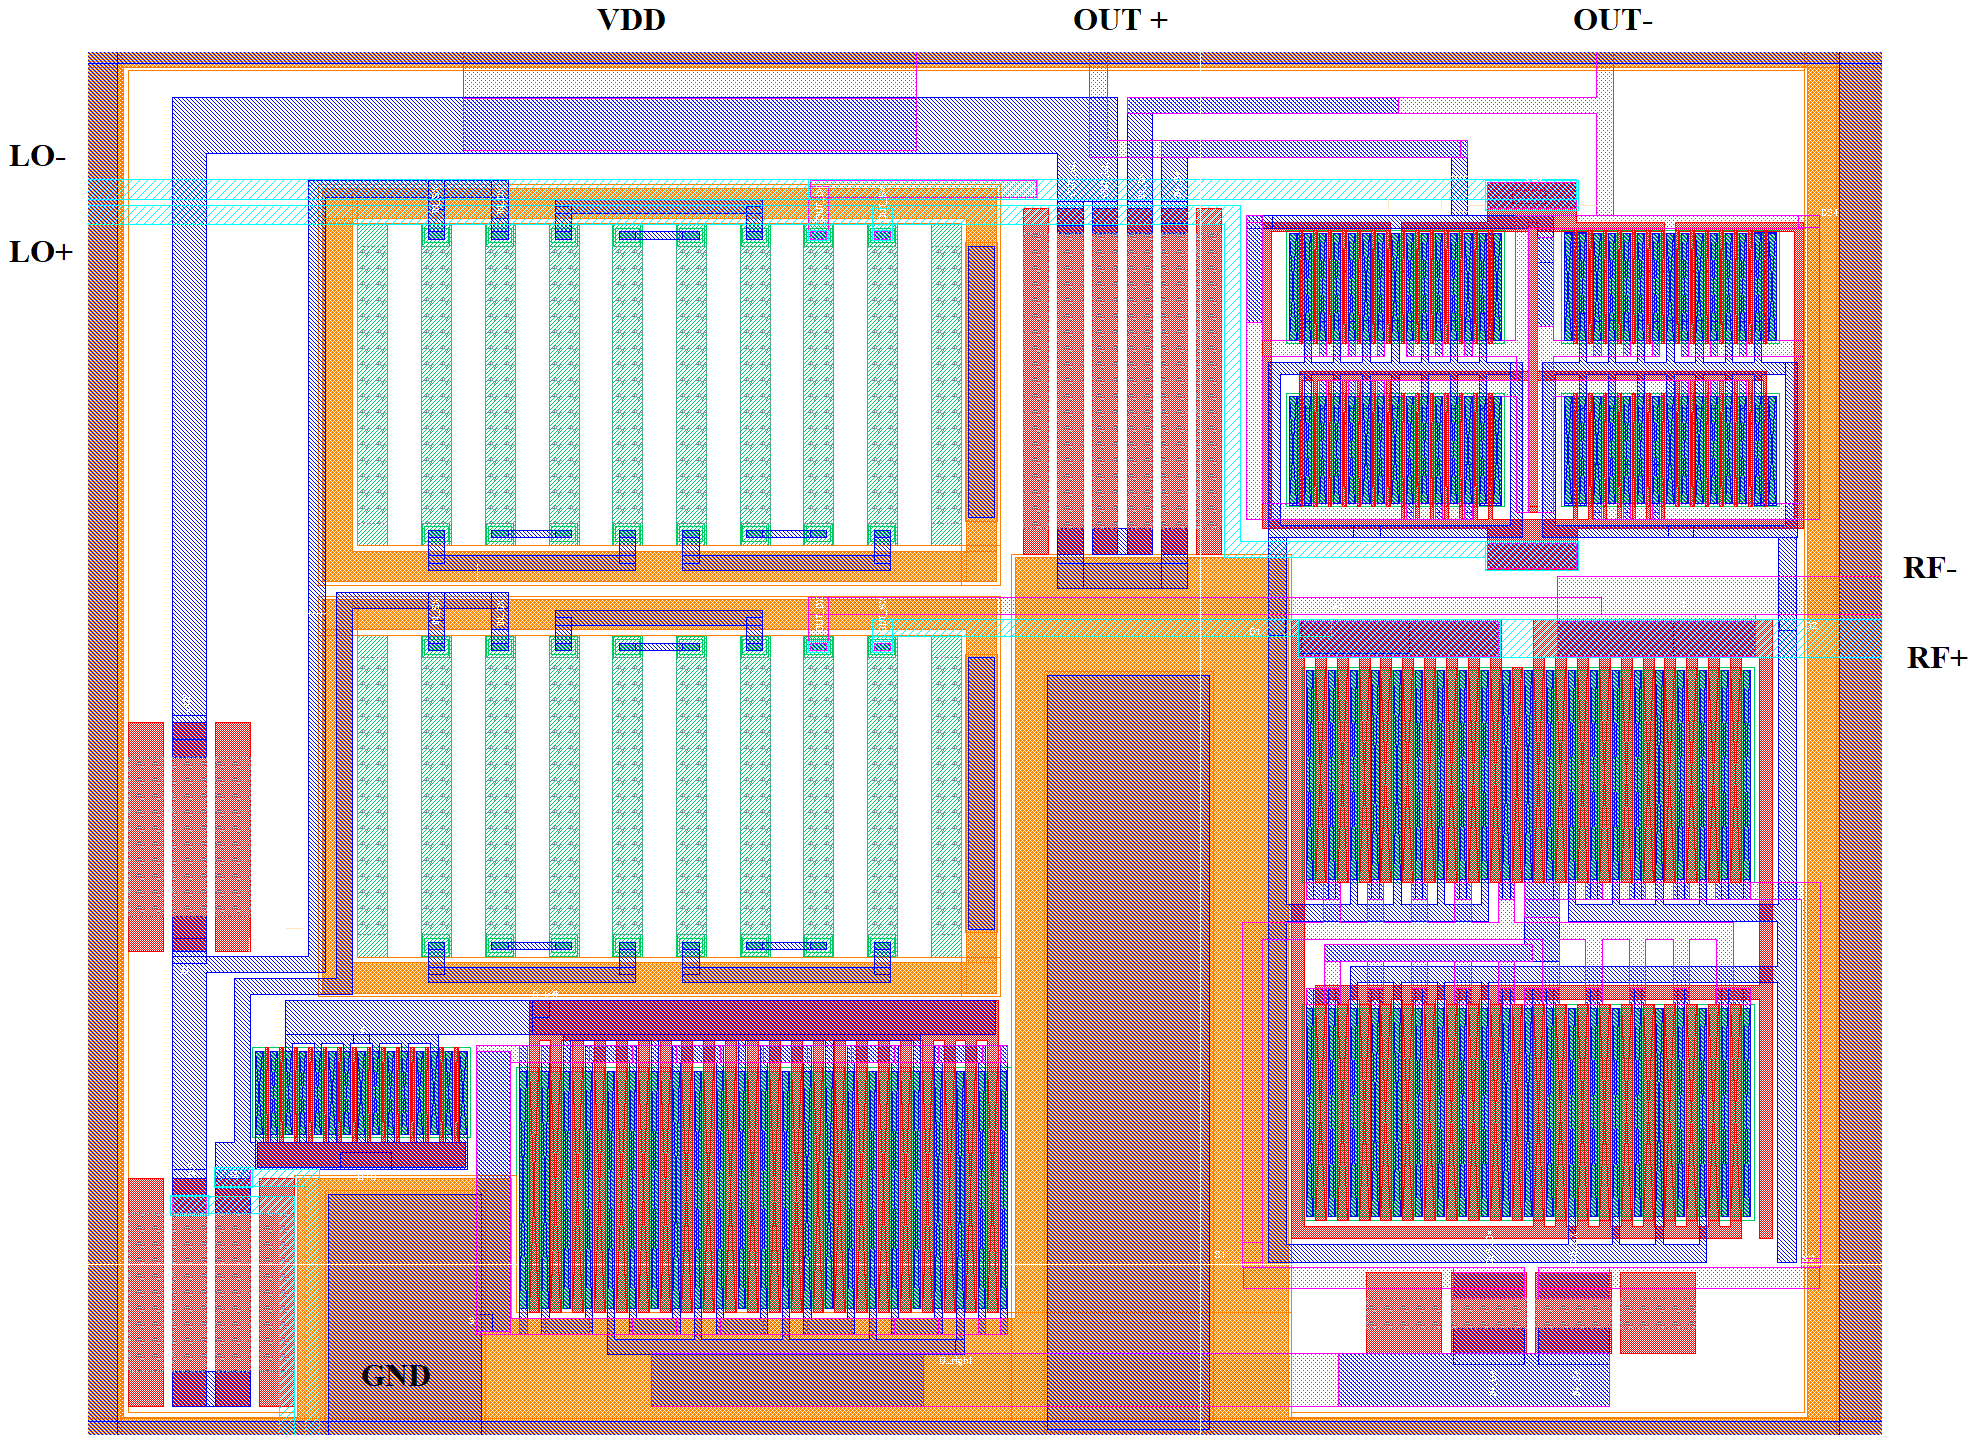
\includegraphics[scale=0.18]{L_complete_zoom}
		\label{L_complete_zoom}
	\end{figure}
\end{frame} 
%--------------------------------------------------------------------------
% 	NEW SUBSECTION
%--------------------------------------------------------------------------
\section{Simulation vs schematic}
\subsection{Simulation setup}

\begin{frame}
	\tableofcontents[currentsubsection]
\end{frame}

\begin{frame}
\frametitle{Analysis}
	Developed analysis:
	\begin{itemize}
		\item Bandwidth;
		\item Time domain output mixed signal and spectral components;
			\item Oscillator signal amplitude to maximize output component;
		\item Conversion gain and 1dB compression point;
		\item Single tone IIP\textsubscript{3};
		\item Two tone IIP\textsubscript{3} and CIM\textsubscript{3};
	\end{itemize}
	Used frequencies: f\textsubscript{LO}=110MHz, f\textsubscript{RF}=100MHz, with expected f\textsubscript{IF}=10MHz.
\end{frame}

\begin{frame}
	\frametitle{Simulation setup}
	\begin{figure}[H]
		\centering
		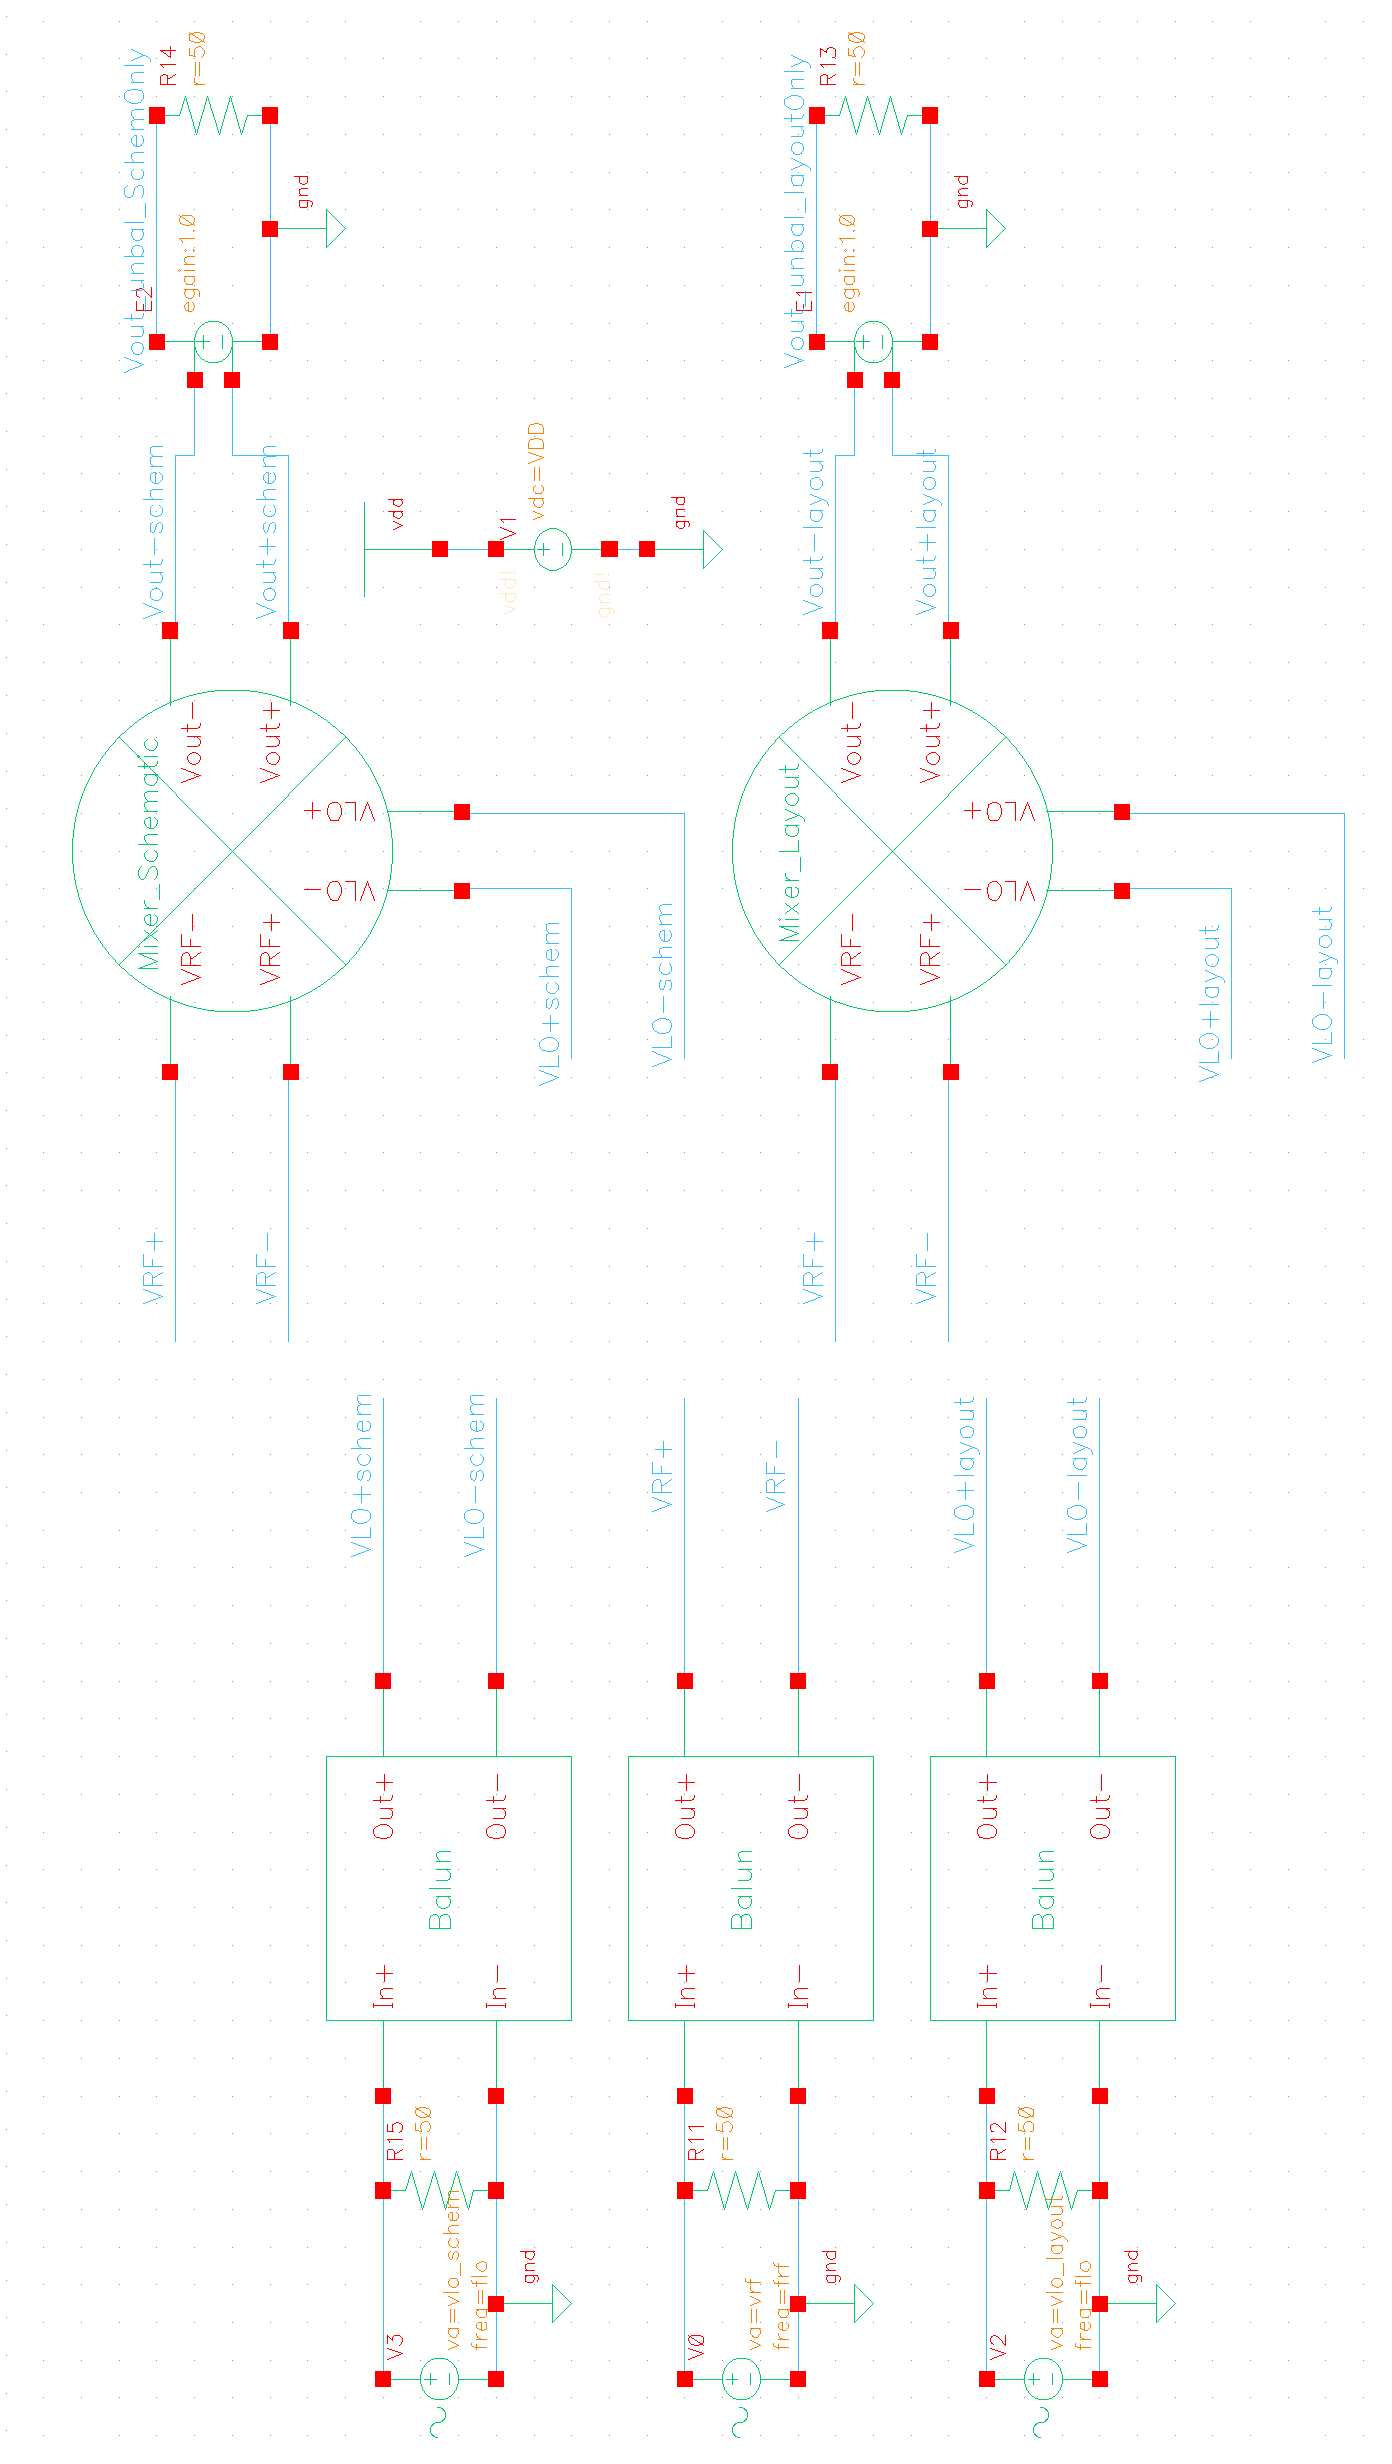
\includegraphics[scale=0.18, angle=-90]{setup}
		\label{fig:setup}
	\end{figure}
\end{frame}

\begin{frame}
	\frametitle{Simulation setup}
	\begin{figure}[H]
		\centering
		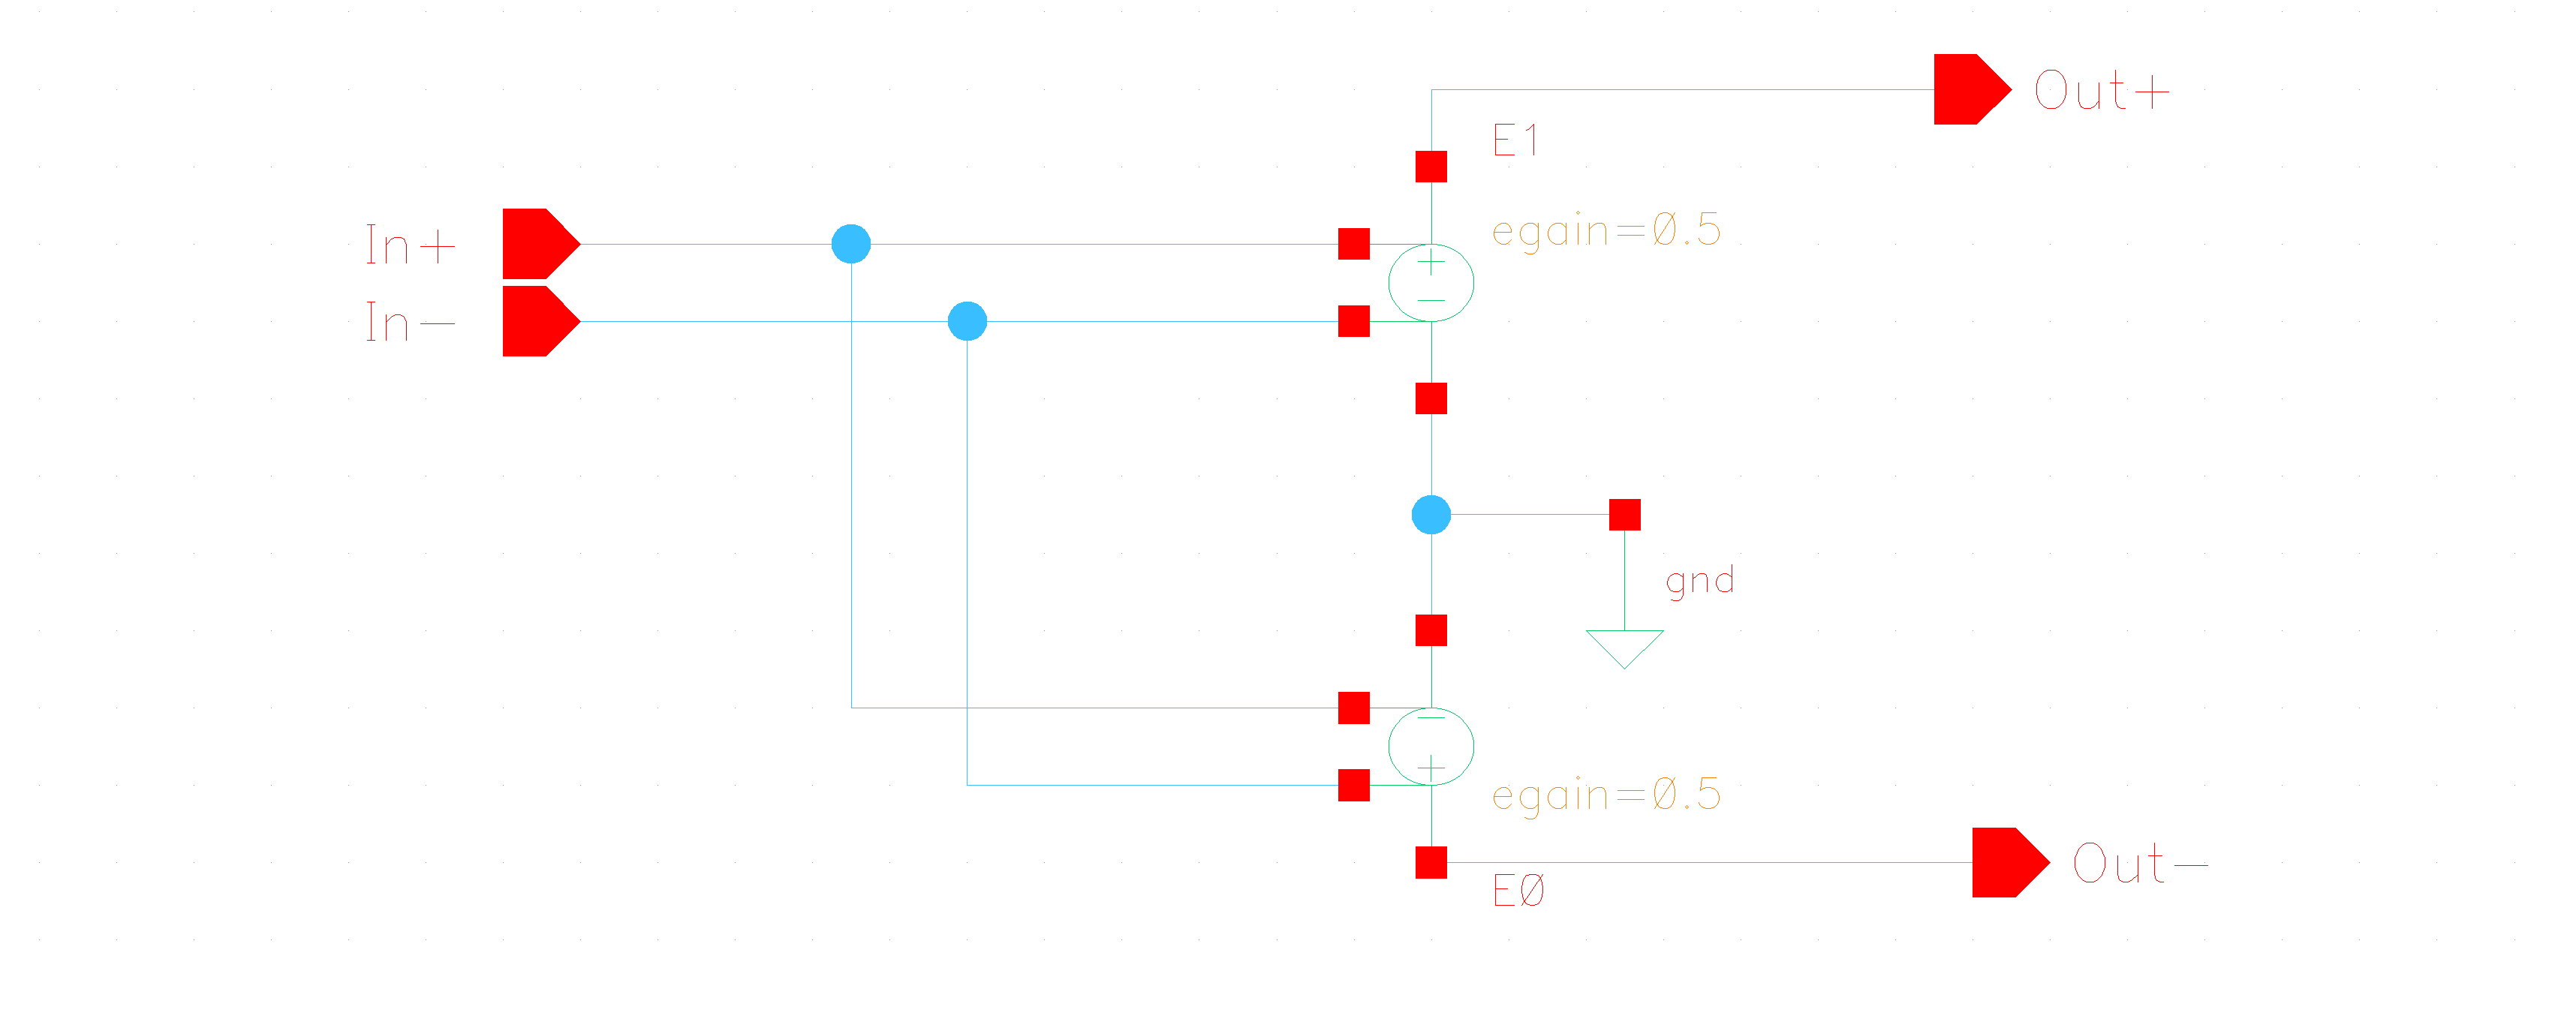
\includegraphics[scale=0.05]{balun}
		\caption{Balun schematic.}
		\label{fig:balun}
	\end{figure}
	\begin{itemize}
		\item Ideal baluns simulate a  50 \(\Omega\) impedance matching condition and differential inputs. 
		\item Mixer's loads, represented by 50\(\Omega\) resistors connected to unitary gain driven generators. Used both for ideal impedance matching purposes and to convert differential output from mixers to single-ended.
	\end{itemize}
\end{frame}

%--------------------------------------------------------------------------
% 	NEW SUBSECTION
%--------------------------------------------------------------------------
\subsection{Time and frequency domain analysis}
\begin{frame}
\tableofcontents[currentsubsection]
\end{frame}

%new slide
\begin{frame}
	\frametitle{Bandwidth evaluation - Transition frequency}
	Dynamic analysis is complex when dealing with non-linear circuits. The following results try to qualify the circuit in the best way.
	Always monochromatic signals have been used. 
	\begin{columns}
	\column{0.4\textwidth}
	Maximum working frequency $f<f_T/10$.
	From current gain measurements on M\textsubscript{3} and M\textsubscript{6}:
	\begin{gather}
		f_T|_{RF}=9.43GHz \notag \\
		f_T|_{LO}=1.12GHz \notag 
	\end{gather} 
	LO stage limits bandwidth. 
	\column{0.6\textwidth}
	\begin{figure}[H]
		\centering 
		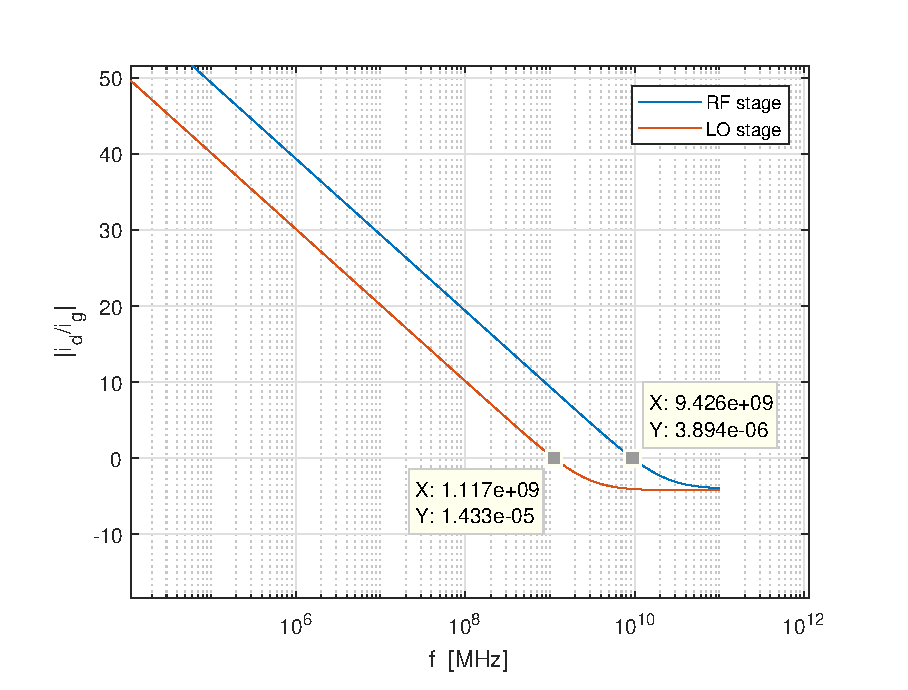
\includegraphics[scale=0.45]{transition_freq}
		\label{fig:ft}
	\end{figure}
	\end{columns}
\end{frame}

\begin{frame}
\frametitle{Bandwidth evaluation - Transition frequency}
\begin{columns}
	\column{0.4\textwidth}
	Bandwidth evaluated by plotting conversion gain dependency on frequency.
	The simulation is performed keeping \(f_{LO}=f_{RF}-10\)MHz.
	-3dB point is located almost two octaves above f\textsubscript{RF}=110MHz.
	
	\column{0.6\textwidth}
	\begin{figure}[H]
		\centering 
		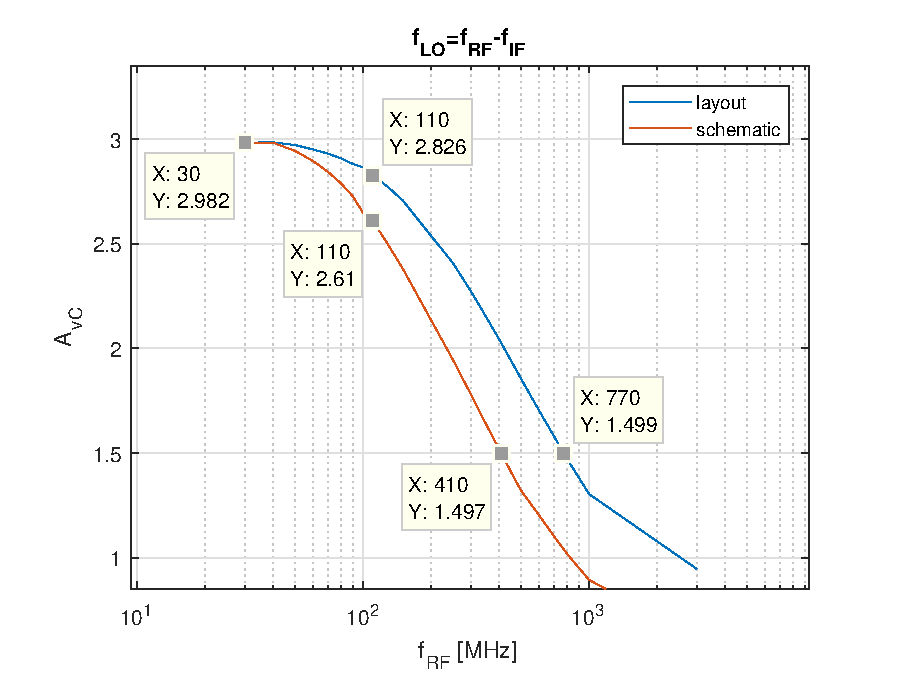
\includegraphics[scale=0.5]{bandwidth}
		\label{fig:band}
	\end{figure}
\end{columns}
\end{frame}

\begin{frame}
	\frametitle{Bandwidth evaluation - Conclusions}
	It is important to notice that we \textbf{cannot rely on this results} because:
	\begin{itemize}
		\item The technology kit is probably not suited for RF operation;
		\item The layout extraction does not account for all device and circuit parasitics, that would affect the performances at high frequency and worsen The physical implementation behaviour;
		\item Pretending accurate results, the simulation emulate the worst case condition. 
	\end{itemize}
\end{frame}

\begin{frame}
\frametitle{Max gain vs LO}
\begin{columns}
	\column{0.4\textwidth}
	LO amplitude must be optimized to get maximum conversion gain. RF power is kept constant, sweeping pump input power.
	
	Layout seems to have better performance than schematic. From simulation:
	\begin{align}
	&V_{LO,opt}|_{layout}=1.23V \notag \\
	&V_{LO,opt}|_{schematic}=2.5V \notag
	\end{align}
	\column{0.6\textwidth}
	\begin{figure}[H]
		\centering
		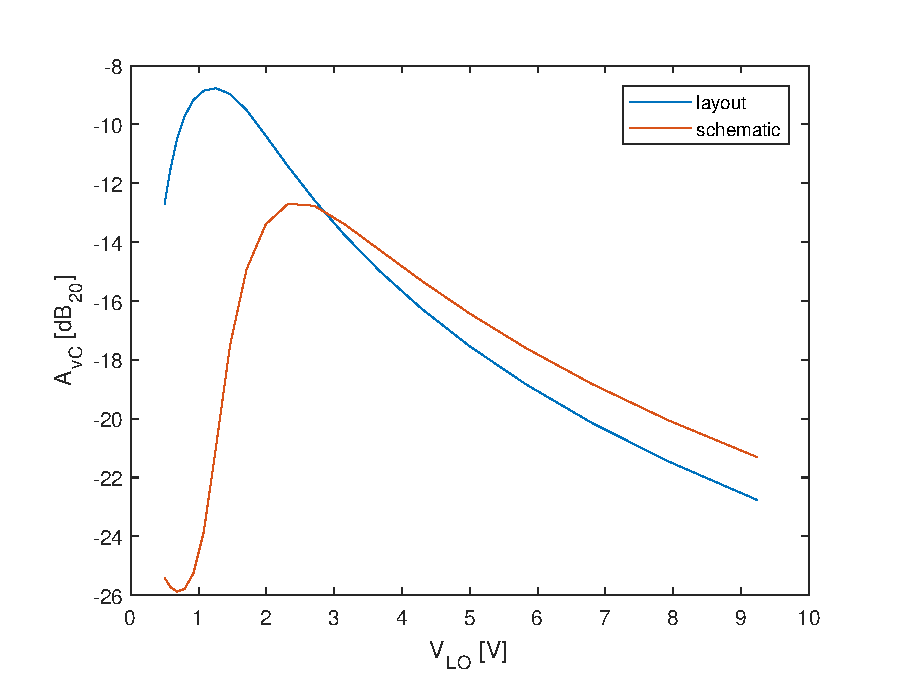
\includegraphics[scale=0.5]{gain_vs_VLO}
		\label{fig:maxGainvsLO}
	\end{figure}
\end{columns}
\end{frame}

\begin{frame}
\frametitle{Time domain analysis}

	\begin{figure}[H]
		\centering
		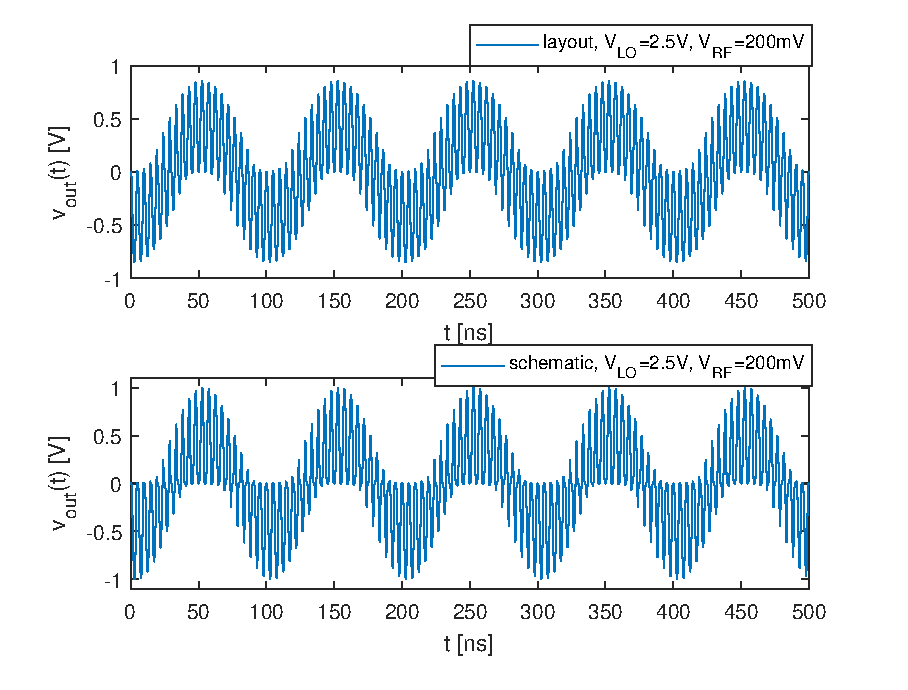
\includegraphics[scale=0.5]{waveforms}
		\caption{Time domain waveforms: double balanced differential output with v\textsubscript{RF}=200mV,  f\textsubscript{RF}=110MHz, v\textsubscript{RF}=1.23mV, f\textsubscript{LO}=100MHz.}
		\label{fig:TdomaniWF}
	\end{figure}

\end{frame}

\begin{frame}
\frametitle{Output signal spectrum}
	\begin{figure}[H]
		\centering
		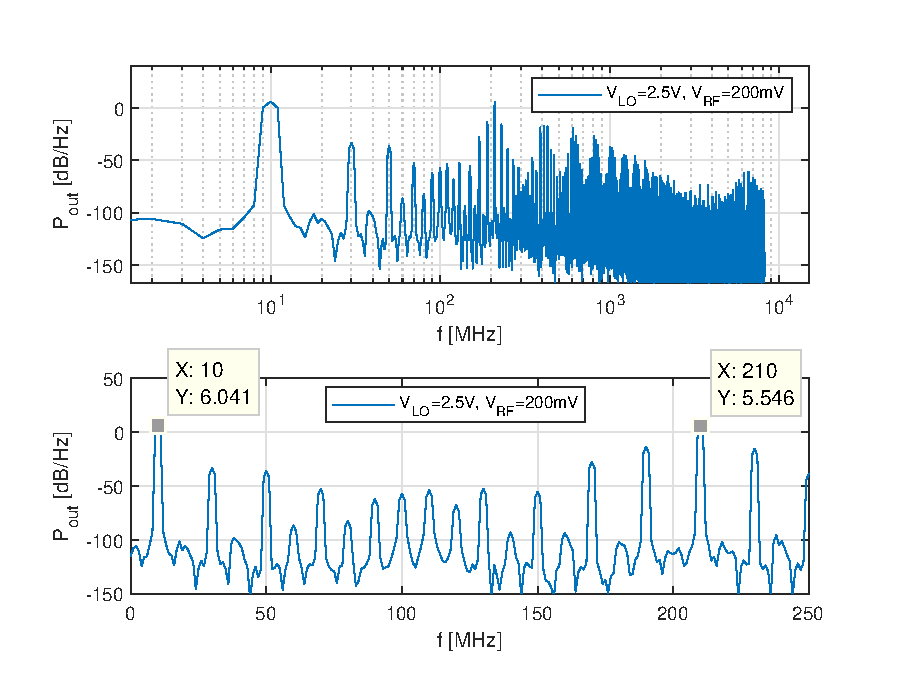
\includegraphics[scale=0.5]{DFT_layout}
		\caption{\textbf{Layout}. Discrete Fourier transform: double balanced differential output with v\textsubscript{RF}=200mV,  f\textsubscript{RF}=110MHz, v\textsubscript{RF}=1.23mV, f\textsubscript{LO}=100MHz,cosine squared smoothing function.}
	\end{figure}
\end{frame}

\begin{frame}
\frametitle{Output signal spectrum}
	\begin{figure}[H]
	\centering
	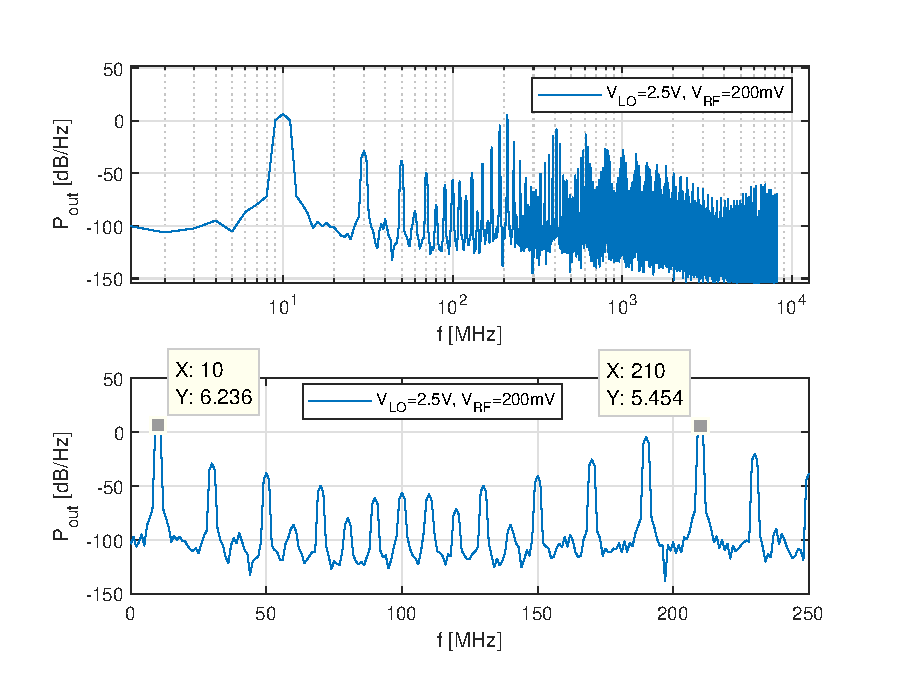
\includegraphics[scale=0.5]{DFT_schem}
	\caption{\textbf{Schematic}. Discrete Fourier transform: double balanced differential output with v\textsubscript{RF}=200mV,  f\textsubscript{RF}=110MHz, v\textsubscript{RF}=1.23mV, f\textsubscript{LO}=100MHz,cosine squared smoothing function.}
	\end{figure}
\end{frame}

\subsection{Power and distortion parameters}
\begin{frame}
\tableofcontents[currentsubsection]
\end{frame}

\begin{frame}
\frametitle{Conversion gain before compression}
\begin{columns}
\column{0.3\textwidth}
Given optimum $V_{LO}=1.23V$, RF voltage was swept to evaluate conversion gain before compression. Obtained conversion gains are as in figure:
\begin{gather}
A_{vC}|_{layout}=2.926 \notag \\ 
A_{vC}|_{schematic}=2.675 \notag
\end{gather}
\column{0.7\textwidth}
\begin{figure}[H]
	\centering
	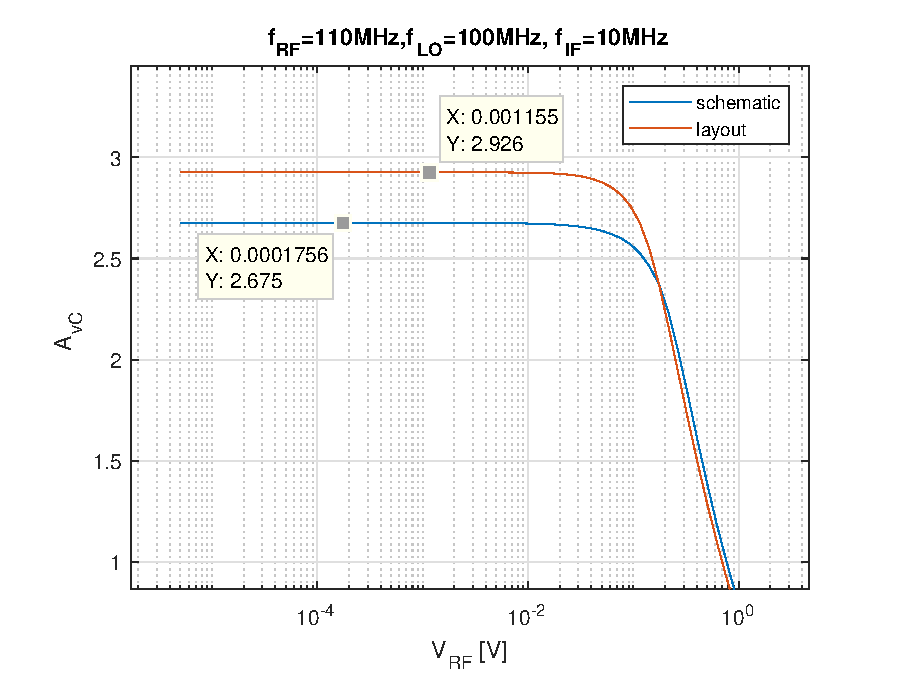
\includegraphics[width=\textwidth]{gain_vs_VRF}
	\caption{Conversion gain vs v\textsubscript{RF}}
	\label{fig:GainvsRF}
\end{figure}
\end{columns}
\end{frame}


\begin{frame}
\frametitle{Single tone $P_{in}$ $P_{out}$}

	\begin{figure}[H] 
		\centering
		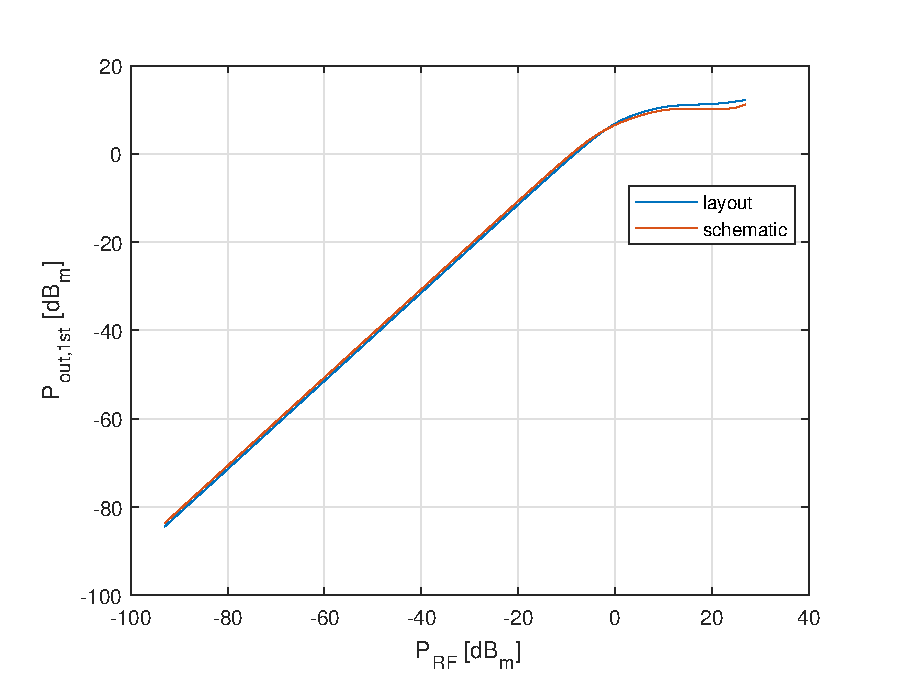
\includegraphics[scale=0.6]{pin_pout_VRF}
		\caption{Single tone $P_{in}$ $P_{out}$ for layout and schematic.}
		\label{fig:PinPout}
	\end{figure}

\end{frame}


\begin{frame}
\frametitle{1dB compression points}
\begin{columns}
	\column{0.4\textwidth}
	RF power for which gains drops of 1dB are equal to 
	\begin{gather}
	P_{RF,in}|_{layout}=-2.3dB_{m} \notag \\
	P_{RF,in}|_{schematic}=-4.8dB_{m} \notag
	\end{gather}
	then, respectively for schematic and layout, the corresponding voltages:
	\begin{gather}
	V_{RF,in}|_{layout}=172mV \notag \\
	V_{RF,in}|_{schematic}=128mV \notag
	\end{gather}
	
	\column{0.6\textwidth}
	\begin{figure}[H] 
		\centering
		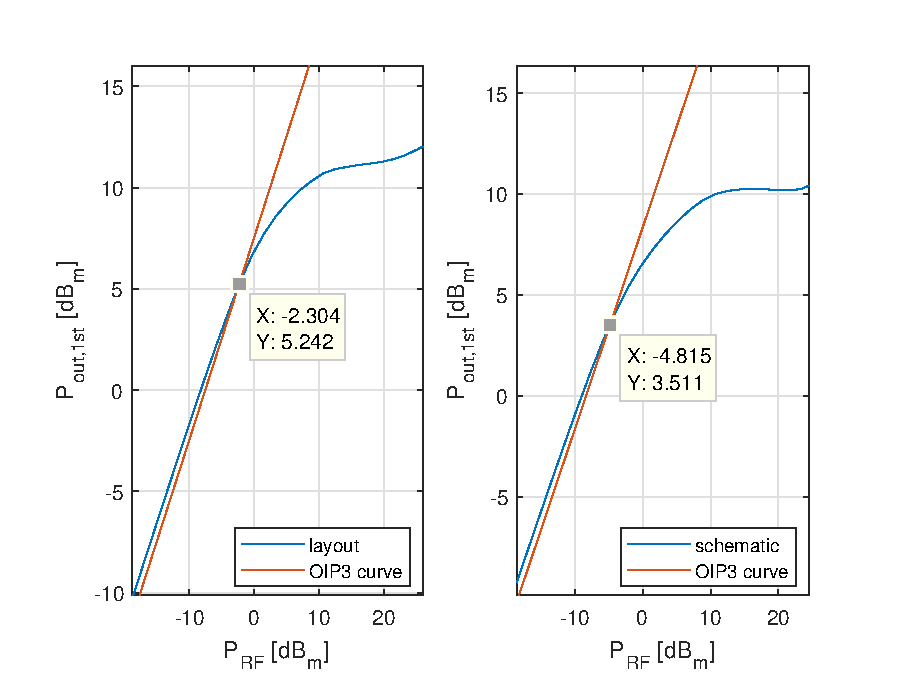
\includegraphics[width=\textwidth]{1dB_compression_1tone}
		\caption{1dB compression point, one-tone analysis}
		\label{fig:PinPout1T_1dBc}
	\end{figure}
\end{columns}
\end{frame}

\begin{frame}
\frametitle{Single tone $3^{rd}$ and $5^{th}$ order distortion}
	Increasing input power, powers of IF's $3^{rd}$ and $5^{th}$ harmonics were measured (most important contributions of output non-linearity at 30MHz and 50MHz). As expected from theory non-linear terms increase with the $3^{rd}$ and $5^{th}$ power of input power.
	\begin{figure}[H] 
		\centering
		\subfloat[][\emph{Harmonics power for schematic}]{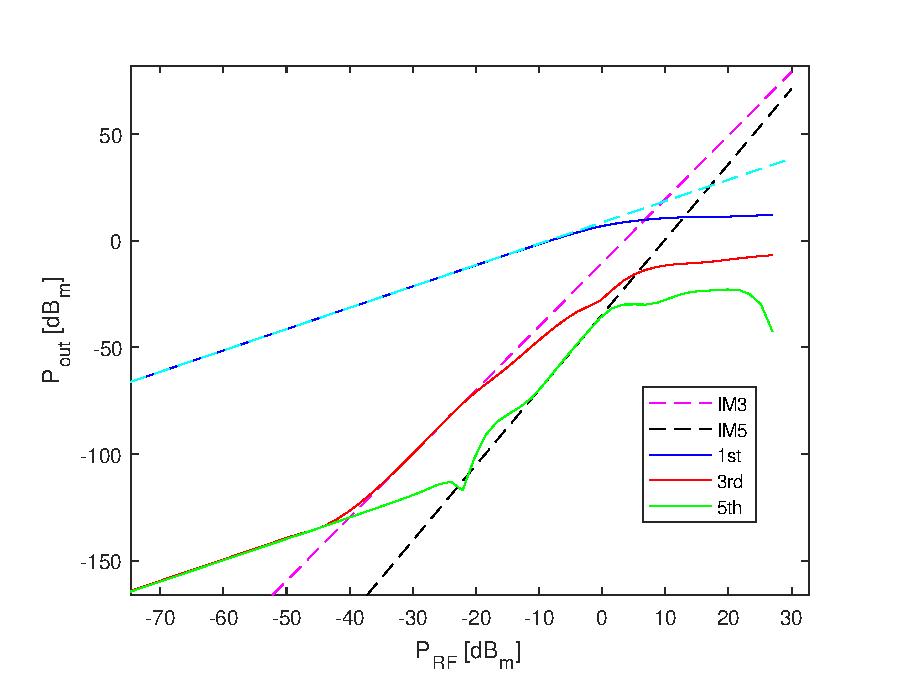
\includegraphics[width=0.5\textwidth,trim=12mm 0mm 0mm 0mm]{IIP3_schem_1tone}}
		\subfloat[][\emph{Harmonics power for layout}]{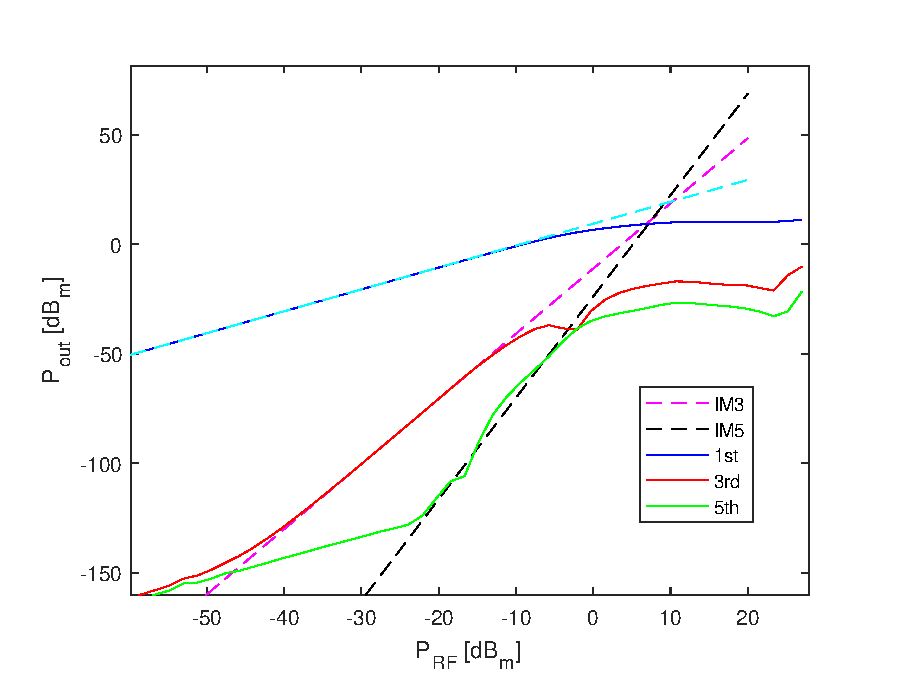
\includegraphics[width=0.5\textwidth,trim=12mm 0mm 0mm 0mm]{IIP3_layout_1tone}}
		\caption{Harmonics power, one tone analysis.}
		\label{fig:IIP3_1t_schem}
	\end{figure}
\end{frame}

\begin{frame}
\frametitle{Input and Output Intercept points}
The amount of distortion is evaluated through the intercept points among the linear regressions of power on fundamental and the ones on harmonics. Coordinates and ordinates are called input and output intercept points (IIP3,IIP5 and OIP3,OIP5).
\begin{figure}[H] 
	\centering
	\subfloat[][\emph{Harmonics power for schematic}]{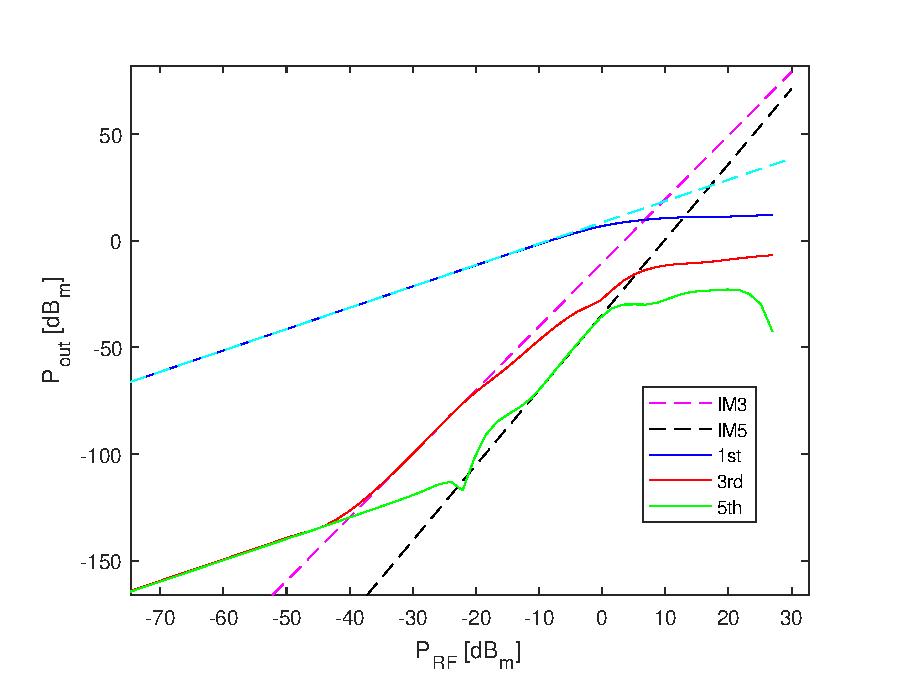
\includegraphics[width=0.5\textwidth,trim=12mm 0mm 0mm 0mm]{IIP3_schem_1tone}}
	\subfloat[][\emph{Harmonics power for layout}]{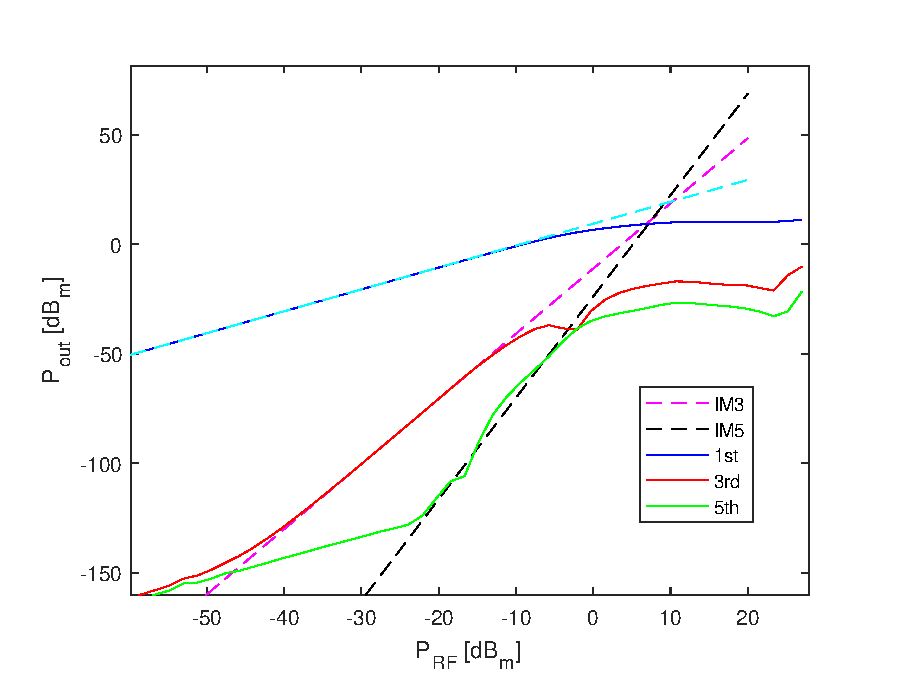
\includegraphics[width=0.5\textwidth,trim=12mm 0mm 0mm 0mm]{IIP3_layout_1tone}}
	\caption{Harmonics power, one tone analysis.}
	\label{fig:IIP3_1t_schem}
\end{figure}
\end{frame}

\begin{frame}
\frametitle{IIP3, IIP5, OIP3, OIP5}
\begin{columns}
	\column{0.5\textwidth}
	IIPs and OIPs measured are shown zooming in on the compression, and reported in table:
	\column{0.4\textwidth}
	\begin{table}[H]
		\label{tab:IIP3_1tone}
		\centering	
		\resizebox{\columnwidth}{!}{%
		\begin{tabular}{lccr} 
			\toprule 
			Parameter & Schematic 	& Layout & unit \\ 
			\midrule
			\(IIP_{3}\)  & 9.73 & 10.4 & dB\(_{m}\) \\
			\(OIP_{3}\)  & 18.3 &19.7 & dB\(_{m}\) \\
			\(IIP_{5}\)  & 17.0 &9.13 & dB\(_{m}\) \\
			\(OIP_{5}\)  & 25.6 &18.5 & dB\(_{m}\) \\
			\bottomrule 
		\end{tabular}	
	}
	\end{table}
	\end{columns}
	\begin{figure}[H] 
		\centering
		\subfloat[][\emph{Schematic detail of IPs}]{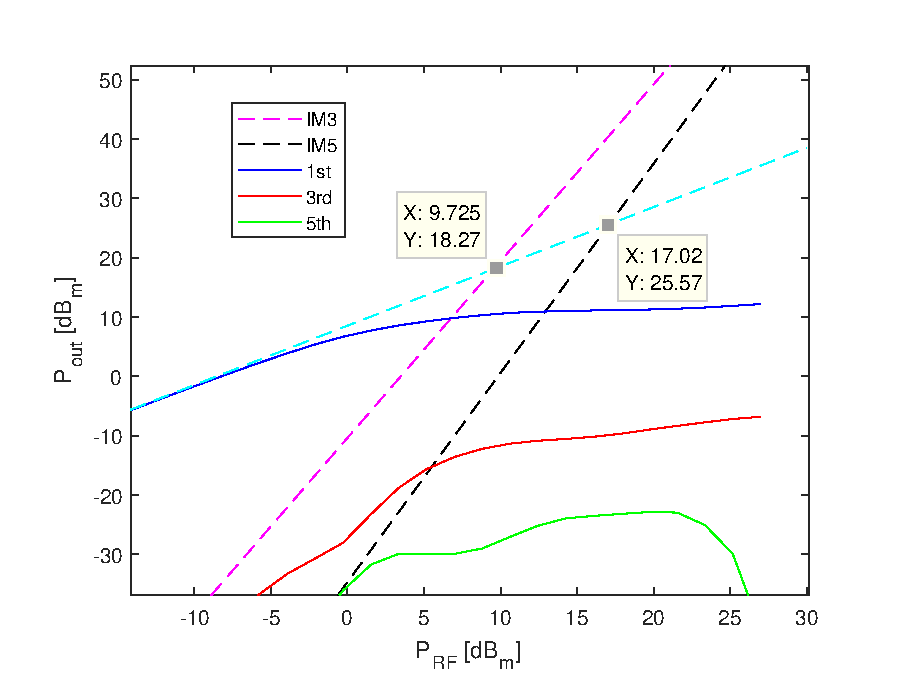
\includegraphics[width=0.5\textwidth,trim= 0mm 0mm 0mm 20mm]{IIP3_schem_1tone_zoom}}
		\subfloat[][\emph{Layout detail of IPs}]{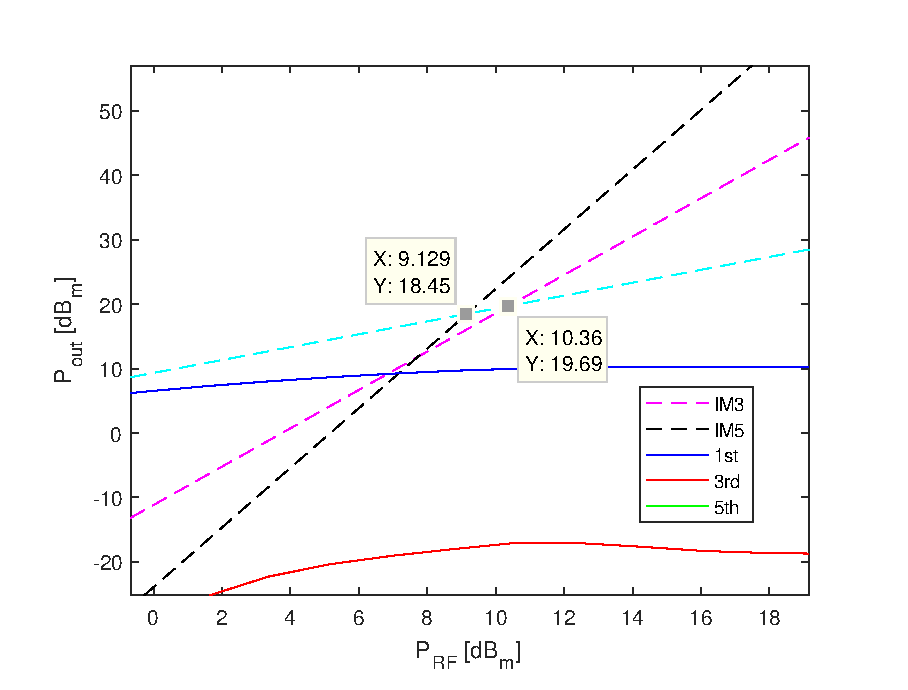
\includegraphics[width=0.5\textwidth,trim= 0mm 0mm 0mm 20mm]{IIP3_layout_1tone_zoom}}
		\label{fig:IIP3_1t_schem}
	\end{figure}
\end{frame}


\begin{frame}
\frametitle{Two tone analysis}
\begin{columns}
	\column{0.45\textwidth}
	 Two tones are injected at 110MHz and 111MHz. In-band IIP\textsubscript{3} result to be at 9MHz and 12MHz. Graphs show that power related to fundamental is strongly reduced when two tones are injected, since power is spread among all intermodulation products.
	\column{0.4\textwidth}
	\begin{figure}[H] 
		\centering
		\subfloat[][\centering\emph{schematic 1dB compression point}]{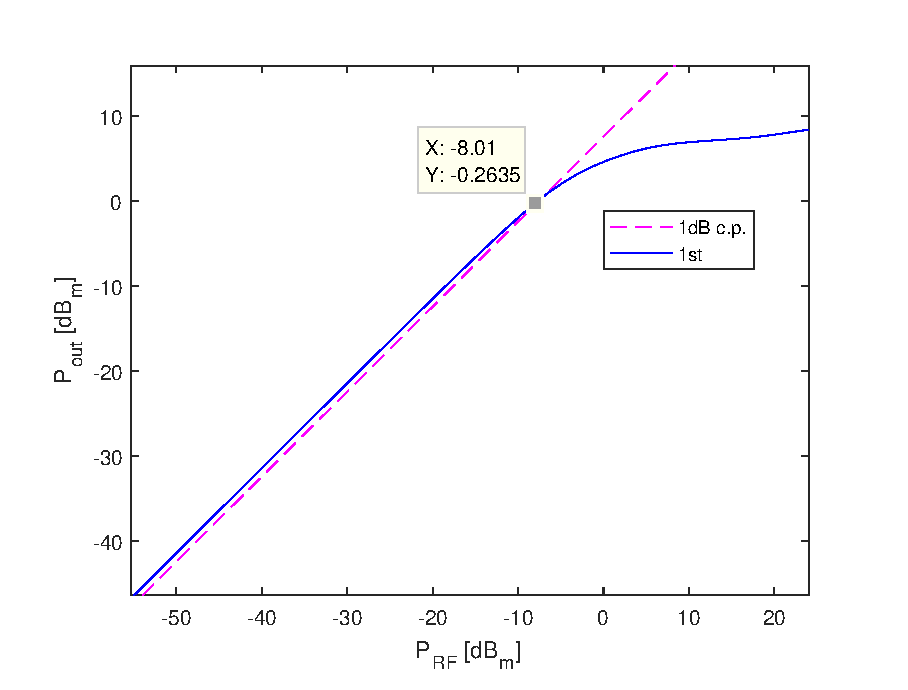
\includegraphics[height=0.3\textheight,trim=0mm 7mm 0mm 8mm, clip=true]{1dB_compression_2tone_schem}}\\
		\subfloat[][\emph{layout}]{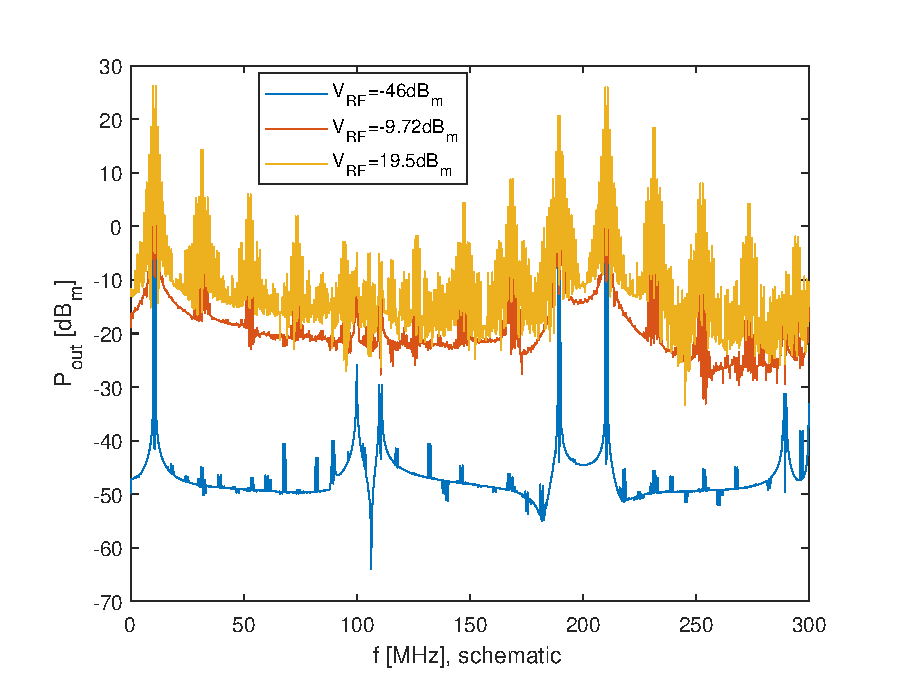
\includegraphics[height=0.3\textheight,trim=0mm 7mm 0mm 8mm, clip=true]{DFT_2tones_schem}}
		\label{fig:1dB_2tones}
	\end{figure}
\end{columns}
\end{frame}


\begin{frame}
\frametitle{Two tone analysis 1dB compression}
	Compression points for both schematic and layout.
	\begin{figure}[H] 
		\centering
		\subfloat[][\emph{schematic}]{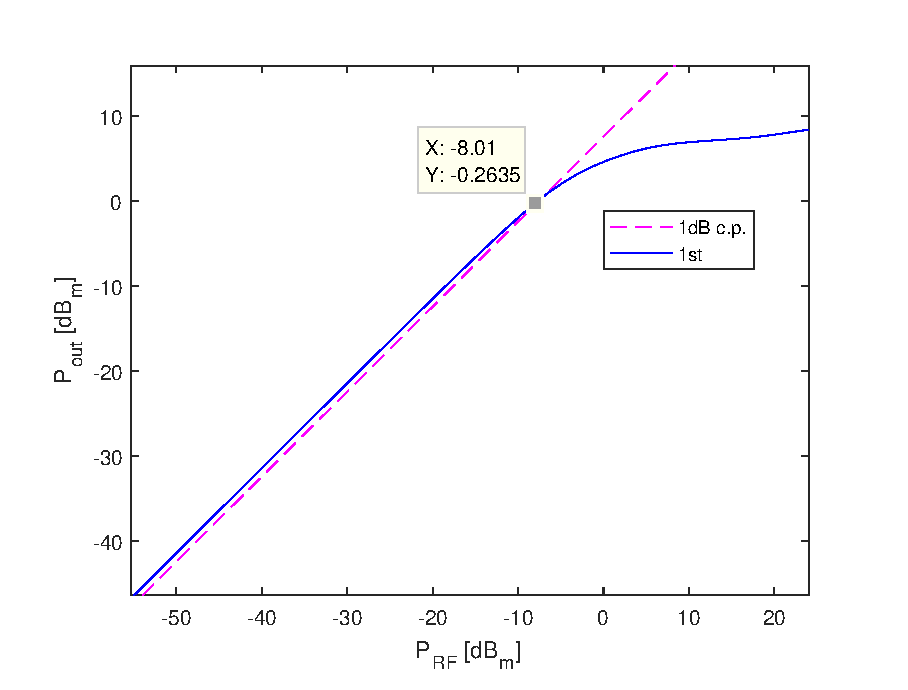
\includegraphics[width=0.5\textwidth]{1dB_compression_2tone_schem}}
		\subfloat[][\emph{layout}]{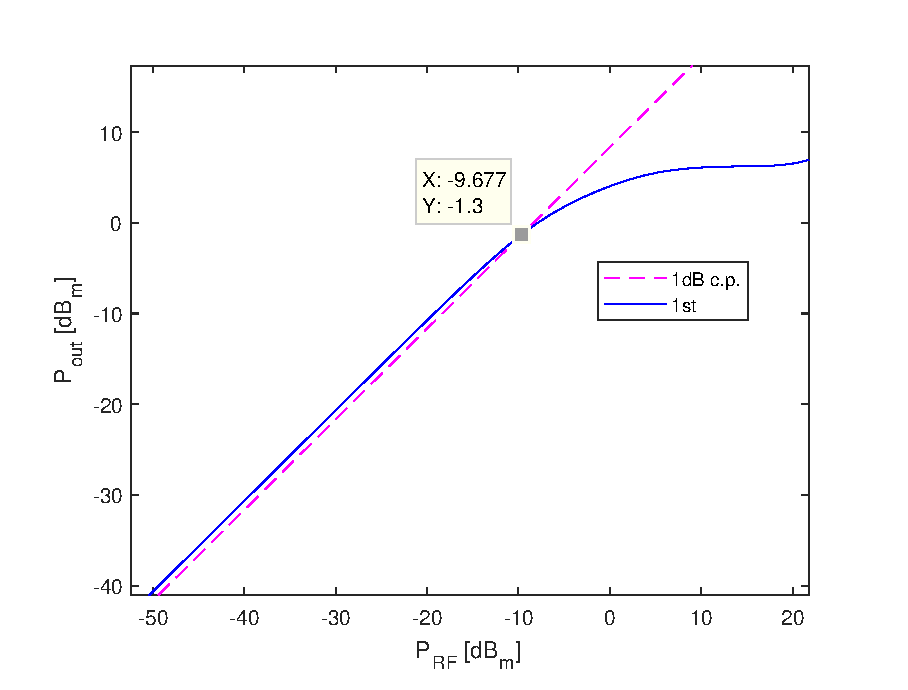
\includegraphics[width=0.5\textwidth]{1dB_compression_2tone_layout}}
		\caption{1dB compression points, two tones.}
		\label{fig:1dB_2tones}
	\end{figure}
\end{frame}


\begin{frame}
\frametitle{Two tone analysis: IM3s'IPs}
Being the power moved from the fundamental to IMPs, input and output intercepts point result lowered with respect the 1-tone case.
\begin{figure}[H] 
	\centering
	\subfloat[][\emph{schematic}]{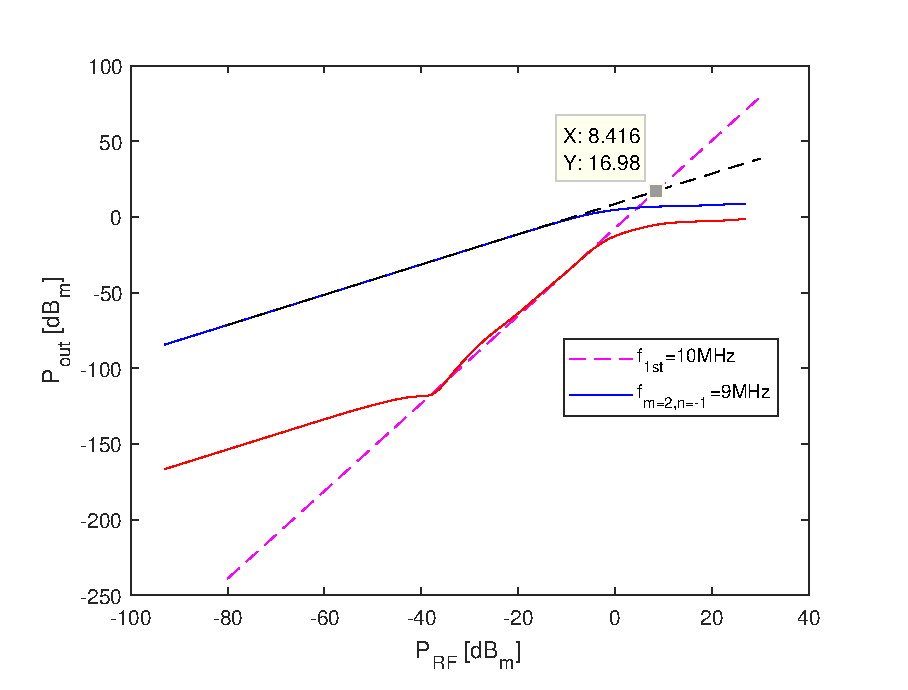
\includegraphics[width=0.5\textwidth]{IIP3_schem_2tone}}
	\subfloat[][\emph{layout}]{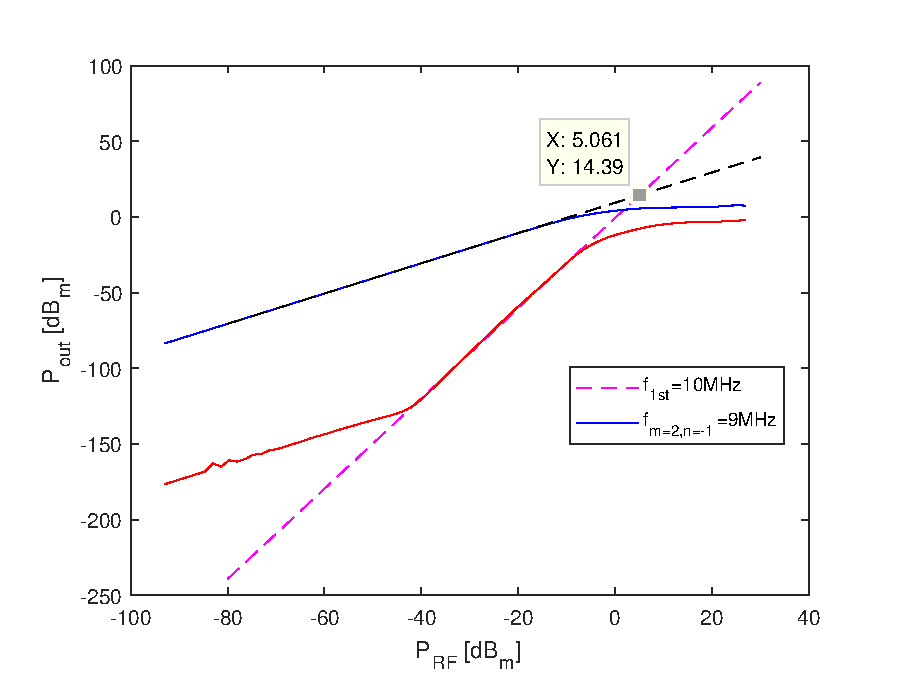
\includegraphics[width=0.5\textwidth]{IIP3_layout_2tone}}
	\caption{Harmonics power, IIP\textsubscript{3} in schematic and layout, two tone analysis.}
	\label{fig:IIP3_2t_schem}
\end{figure}
\end{frame}

\begin{frame}
\frametitle{Two tone analysis: spectra}
Frequency spectra at difference input power have been retrieved for schematic and layout. It is clearly visible the intrinsic rejection of LO and RF frequencies of the Gilbert double balanced cell.
\begin{figure}[H] 
	\centering
	\subfloat[][\emph{schematic}]{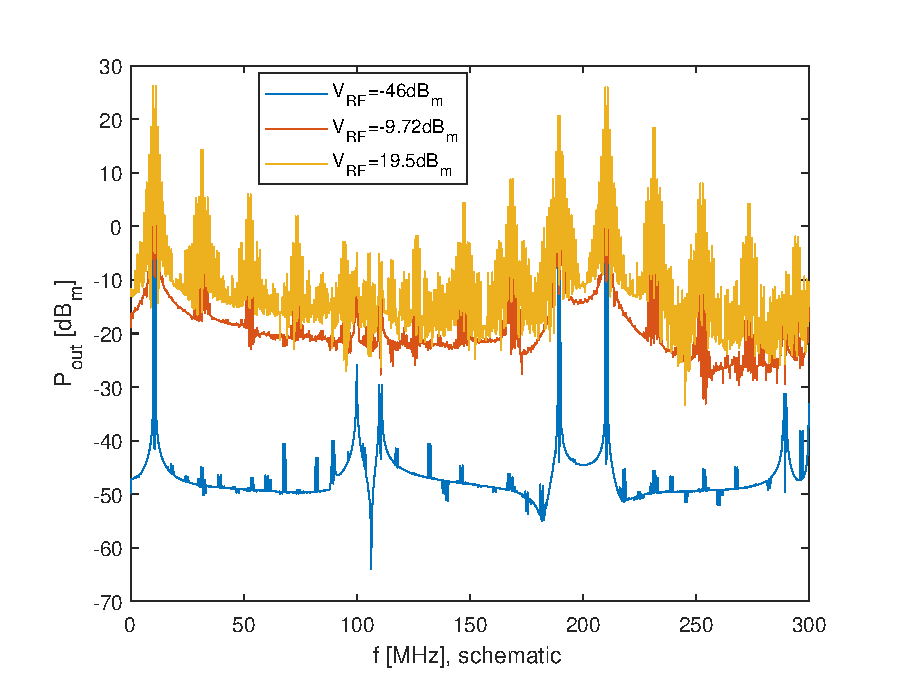
\includegraphics[width=0.5\textwidth]{DFT_2tones_schem}}
	\subfloat[][\emph{layout}]{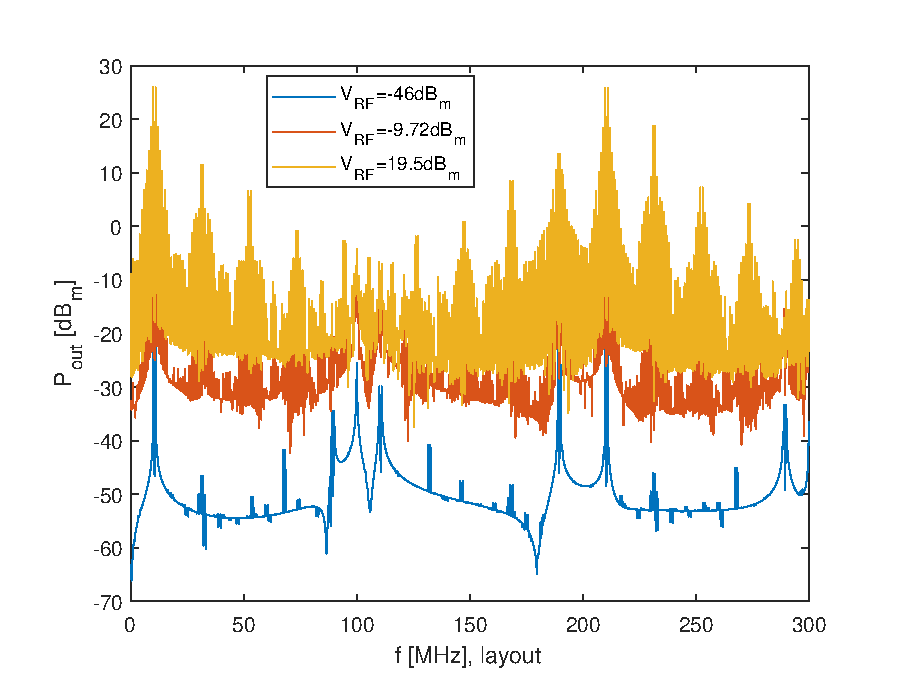
\includegraphics[width=0.5\textwidth]{DFT_2tones_layout}}
	\caption{DFT, comparison between layout and schematic; cosine2 smoothing function.}
	\label{fig:DFT_2ton}
\end{figure}
\end{frame}


\begin{frame}
\frametitle{Two tone analysis: CIM3}
The 1dB compression point spectrum has been chosen (PRF=-9.68dBm) to measure the CIM3 ratio, since this is set as the maximum input power accepted by the multiplier without heavy distortion.
\begin{figure}[H] 
	\centering
	\subfloat[][\emph{schematic}]{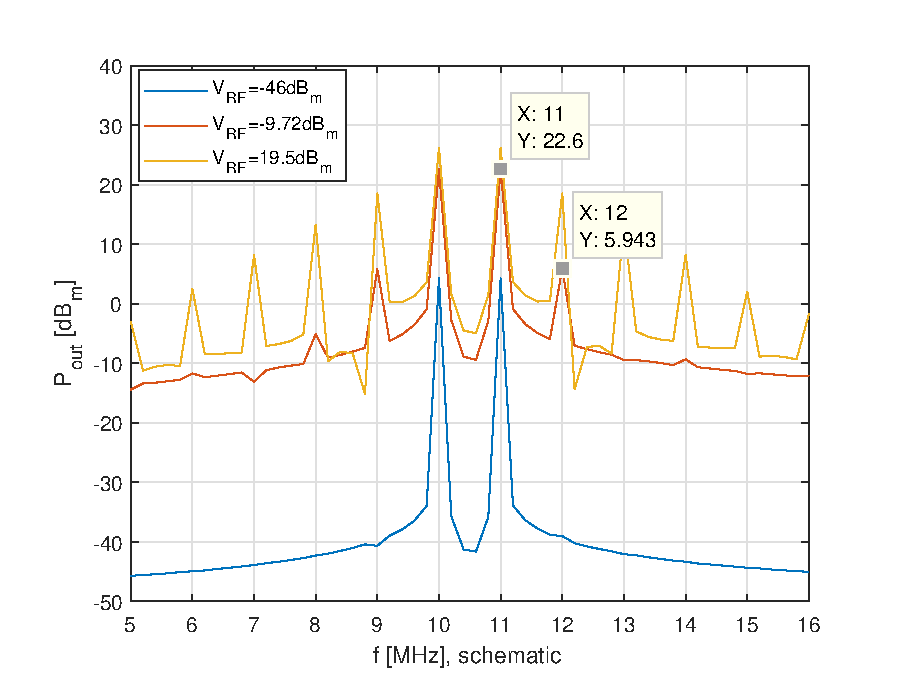
\includegraphics[width=0.5\textwidth]{DFT_2tones_schem_zoom}}
	\subfloat[][\emph{layout}]{\includegraphics[width=0.5\textwidth]{DFT_2tones_layout_zoom}}
	\caption{DFT, comparison between layout and schematic. CIM\textsubscript{3} measurement at 1dB compression point; cosine2 smoothing function. }
	\label{fig:DFT_2ton_zoom}
\end{figure}
\end{frame}

\begin{frame}
\frametitle{Two tone analysis: CIM3}
As it appears, power carried from fundamental tones (10MHz and 11MHz) barely increases after this point, whereas other tones keep increasing. 
\begin{figure}[H] 
	\centering
	\subfloat[][\emph{schematic}]{\includegraphics[width=0.5\textwidth]{DFT_2tones_schem_zoom}}
	\subfloat[][\emph{layout}]{\includegraphics[width=0.5\textwidth]{DFT_2tones_layout_zoom}}
	\caption{DFT, comparison between layout and schematic. CIM\textsubscript{3} measurement at 1dB compression point; cosine2 smoothing function. }
	\label{fig:DFT_2ton_zoom}
\end{figure}
\end{frame}

\begin{frame}
\frametitle{Two tone analysis: Summing up}
The table with summarized results for the analysis is reported below. Overall, the layout looks less performing as expected. 
\begin{figure}[H] 
	\centering
	\subfloat[][\emph{schematic}]{\includegraphics[width=0.5\textwidth]{DFT_2tones_schem_zoom}}
	\subfloat[][\emph{layout}]{\includegraphics[width=0.5\textwidth]{DFT_2tones_layout_zoom}}
	\caption{DFT, comparison between layout and schematic. CIM\textsubscript{3} measurement at 1dB compression point; cosine2 smoothing function. }
	\label{fig:DFT_2ton_zoom}
\end{figure}
\end{frame} 
\section{Conclusions}
\begin{frame}
\tableofcontents[currentsection]
\end{frame}

\begin{frame}
\frametitle{Conclusions}
Good news:
\begin{itemize}
	\item The circuit correctly mixes;
	\item Reasonable conversion gain (A\textsubscript{v,layout} $\simeq$ 2.9, A\textsubscript{v,schem} $\simeq$ 2.7) with good matching between simulations and hand calculations;
	\item Acceptable amount of distortion if the input power remains well below the 1dB compression point ($\simeq$100mV);
\end{itemize}
\end{frame}

\begin{frame}
\frametitle{Conclusions}
Bad news:
\begin{itemize}
	\item The AMI's 0.6 by MOSIS is old-fashioned, not meant for RF applications;
	\item The extractor used to generate the layout (Cadence Diva) was not able to provide the full set of parasitic elements, leading to inaccurate analysis;
	\item Wide circuit area necessary to fulfil the specifications (gain, power consumption), this produces a large amount of parasitic elements.  
\end{itemize}
To sum up, the circuit functions properly, although it probably \textbf{overestimates} what would be the real behaviour. 

\end{frame}

\begin{frame}
\nocite{*}
\bibliography{References1}{}
\bibliographystyle{plain}
\end{frame}

 
%%------------------------------------------------
\section*{First Section} % Sections can be created in order to organize your presentation into discrete blocks, all sections and subsections are automatically printed in the table of contents as an overview of the talk
%------------------------------------------------

\subsection*{Subsection Example} % A subsection can be created just before a set of slides with a common theme to further break down your presentation into chunks

\begin{frame}
\frametitle{Paragraphs of Text}
Sed iaculis dapibus gravida. Morbi sed tortor erat, nec interdum arcu. Sed id lorem lectus. Quisque viverra augue id sem ornare non aliquam nibh tristique. Aenean in ligula nisl. Nulla sed tellus ipsum. Donec vestibulum ligula non lorem vulputate fermentum accumsan neque mollis.\\~\\

Sed diam enim, sagittis nec condimentum sit amet, ullamcorper sit amet libero. Aliquam vel dui orci, a porta odio. Nullam id suscipit ipsum. Aenean lobortis commodo sem, ut commodo leo gravida vitae. Pellentesque vehicula ante iaculis arcu pretium rutrum eget sit amet purus. Integer ornare nulla quis neque ultrices lobortis. Vestibulum ultrices tincidunt libero, quis commodo erat ullamcorper id.
\end{frame}

%------------------------------------------------

\begin{frame}
\frametitle{Bullet Points}
\begin{itemize}
\item Lorem ipsum dolor sit amet, consectetur adipiscing elit
\item Aliquam blandit faucibus nisi, sit amet dapibus enim tempus eu
\item Nulla commodo, erat quis gravida posuere, elit lacus lobortis est, quis porttitor odio mauris at libero
\item Nam cursus est eget velit posuere pellentesque
\item Vestibulum faucibus velit a augue condimentum quis convallis nulla gravida
\end{itemize}
\end{frame}

%------------------------------------------------

\begin{frame}
\frametitle{Blocks of Highlighted Text}
\begin{block}{Block 1}
Lorem ipsum dolor sit amet, consectetur adipiscing elit. Integer lectus nisl, ultricies in feugiat rutrum, porttitor sit amet augue. Aliquam ut tortor mauris. Sed volutpat ante purus, quis accumsan dolor.
\end{block}

\begin{block}{Block 2}
Pellentesque sed tellus purus. Class aptent taciti sociosqu ad litora torquent per conubia nostra, per inceptos himenaeos. Vestibulum quis magna at risus dictum tempor eu vitae velit.
\end{block}

\begin{block}{Block 3}
Suspendisse tincidunt sagittis gravida. Curabitur condimentum, enim sed venenatis rutrum, ipsum neque consectetur orci, sed blandit justo nisi ac lacus.
\end{block}
\end{frame}

%------------------------------------------------

\begin{frame}
\frametitle{Multiple Columns}
\begin{columns}[c] % The "c" option specifies centered vertical alignment while the "t" option is used for top vertical alignment

\column{.45\textwidth} % Left column and width
\textbf{Heading}
\begin{enumerate}
\item Statement
\item Explanation
\item Example
\end{enumerate}

\column{.5\textwidth} % Right column and width
Lorem ipsum dolor sit amet, consectetur adipiscing elit. Integer lectus nisl, ultricies in feugiat rutrum, porttitor sit amet augue. Aliquam ut tortor mauris. Sed volutpat ante purus, quis accumsan dolor.

\end{columns}
\end{frame}

%------------------------------------------------
\section*{Second Section}
%------------------------------------------------

\begin{frame}
\frametitle{Table}
\begin{table}
\begin{tabular}{l l l}
\toprule
\textbf{Treatments} & \textbf{Response 1} & \textbf{Response 2}\\
\midrule
Treatment 1 & 0.0003262 & 0.562 \\
Treatment 2 & 0.0015681 & 0.910 \\
Treatment 3 & 0.0009271 & 0.296 \\
\bottomrule
\end{tabular}
\caption{Table caption}
\end{table}
\end{frame}

%------------------------------------------------

\begin{frame}
\frametitle{Theorem}
\begin{theorem}[Mass--energy equivalence]
$E = mc^2$
\end{theorem}
\end{frame}

%------------------------------------------------

\begin{frame}[fragile] % Need to use the fragile option when verbatim is used in the slide
\frametitle{Verbatim}
\begin{example}[Theorem Slide Code]
\begin{verbatim}
\begin{frame}
\frametitle{Theorem}
\begin{theorem}[Mass--energy equivalence]
$E = mc^2$
\end{theorem}
\end{frame}\end{verbatim}
\end{example}
\end{frame}

%------------------------------------------------

\begin{frame}
\frametitle{Figure}
Uncomment the code on this slide to include your own image from the same directory as the template .TeX file.
%\begin{figure}
%\includegraphics[width=0.8\linewidth]{test}
%\end{figure}
\end{frame}

%------------------------------------------------

\begin{frame}[fragile] % Need to use the fragile option when verbatim is used in the slide
\frametitle{Citation}
An example of the \verb|\cite| command to cite within the presentation:\\~

This statement requires citation \cite{p1}.
\end{frame}

%------------------------------------------------

\begin{frame}
\frametitle{References}
\footnotesize{
\begin{thebibliography}{99} % Beamer does not support BibTeX so references must be inserted manually as below
\bibitem[Smith, 2012]{p1} John Smith (2012)
\newblock Title of the publication
\newblock \emph{Journal Name} 12(3), 45 -- 678.
\end{thebibliography}
}
\end{frame}

%------------------------------------------------

\begin{frame}
\Huge{\centerline{The End}}
\end{frame}

%----------------------------------------------------------------------------------------

\end{document}